\section{机器学习}
\textcolor{main1}{符号主义的困境}
\begin{figure}[htbp]
    \centering
    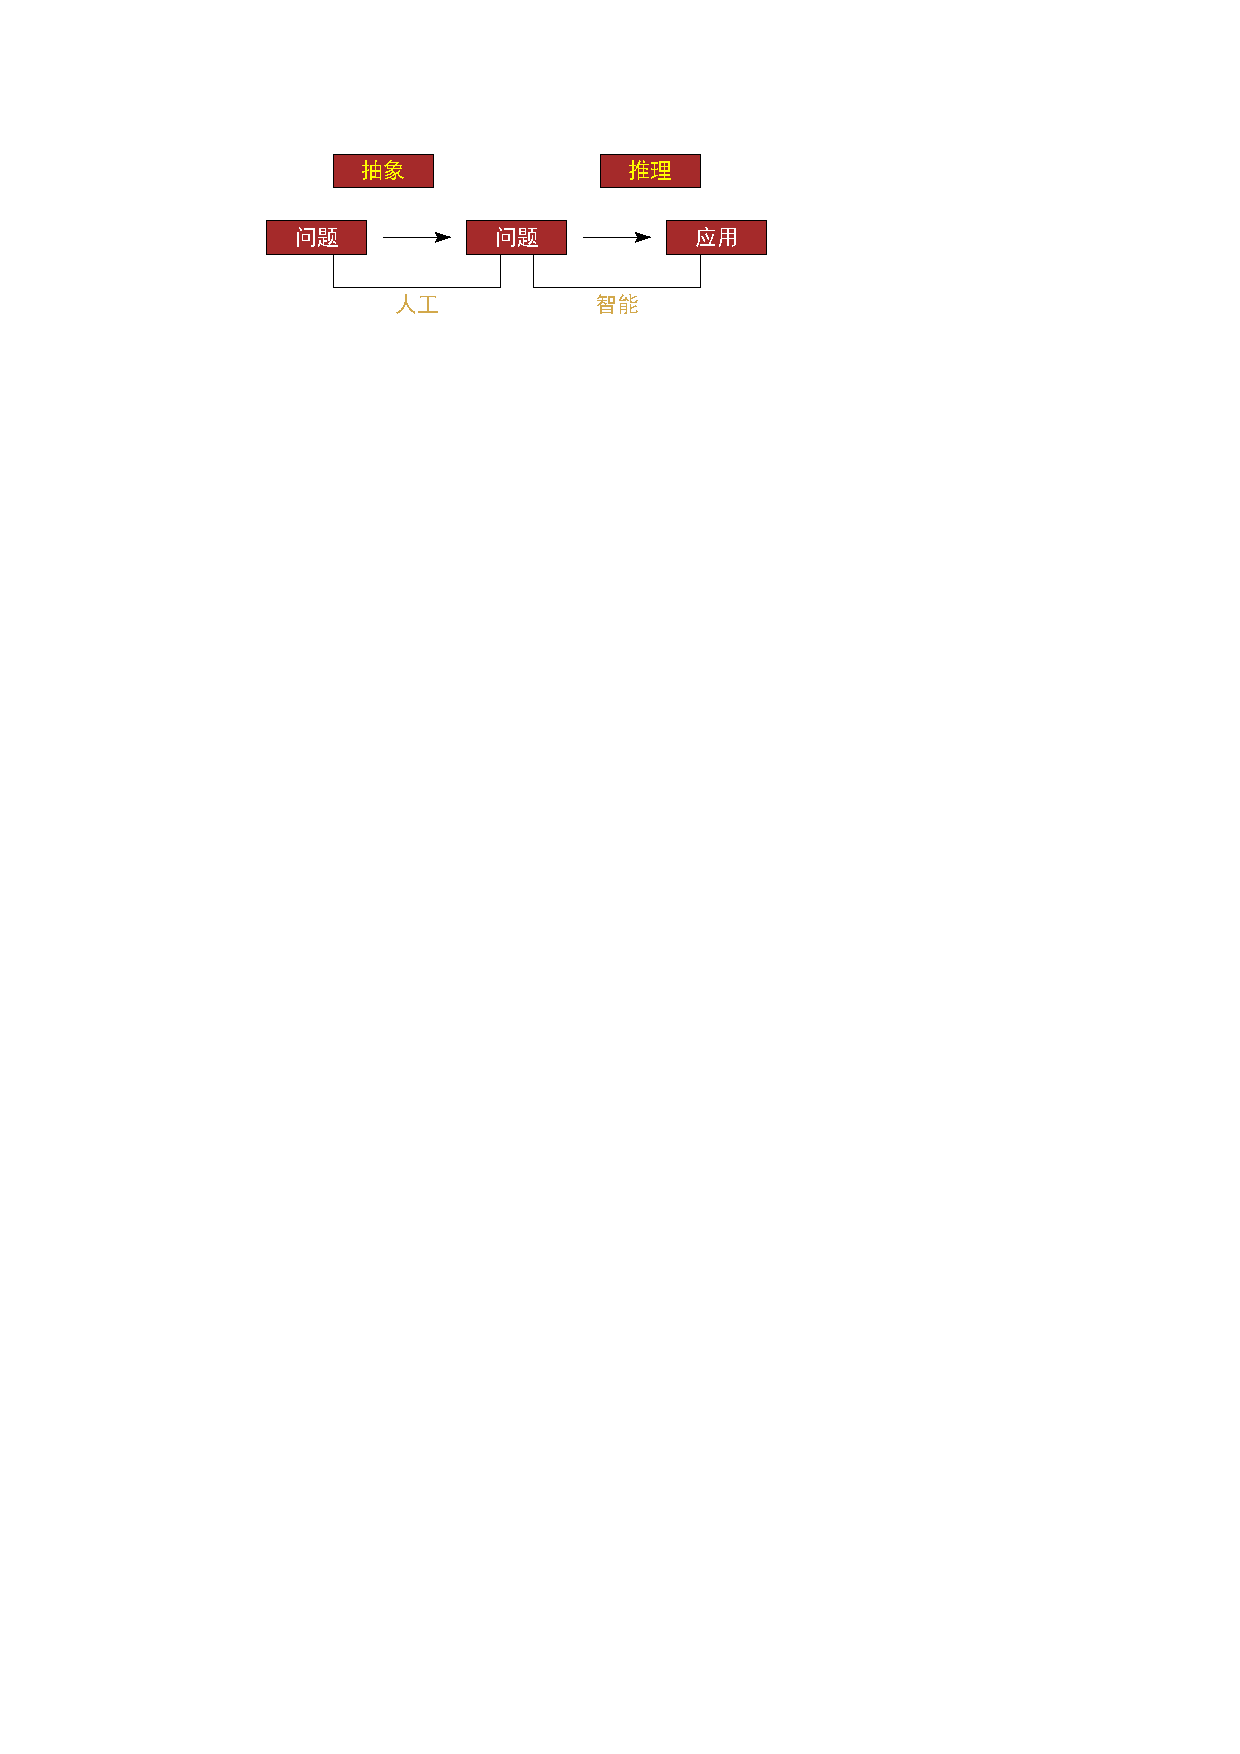
\includegraphics{image/符号主义的困境.pdf}
\end{figure}
\begin{itemize}
    \item 将问题抽象为模型的过程(知识表示)需要人工完成。把知识总结出来再交给计算机相当困难,存在知识获取瓶颈。
    \item \textcolor{main1}{很多涉及大量数据和多变量的复杂问题,没有现成的推理规则和处理方式。}
\end{itemize}

\subsection{机器学习概述}
\subsubsection{基本概念}
\textcolor{main1}{两种通用的学习类型}
\begin{figure}[htbp]
    \centering
    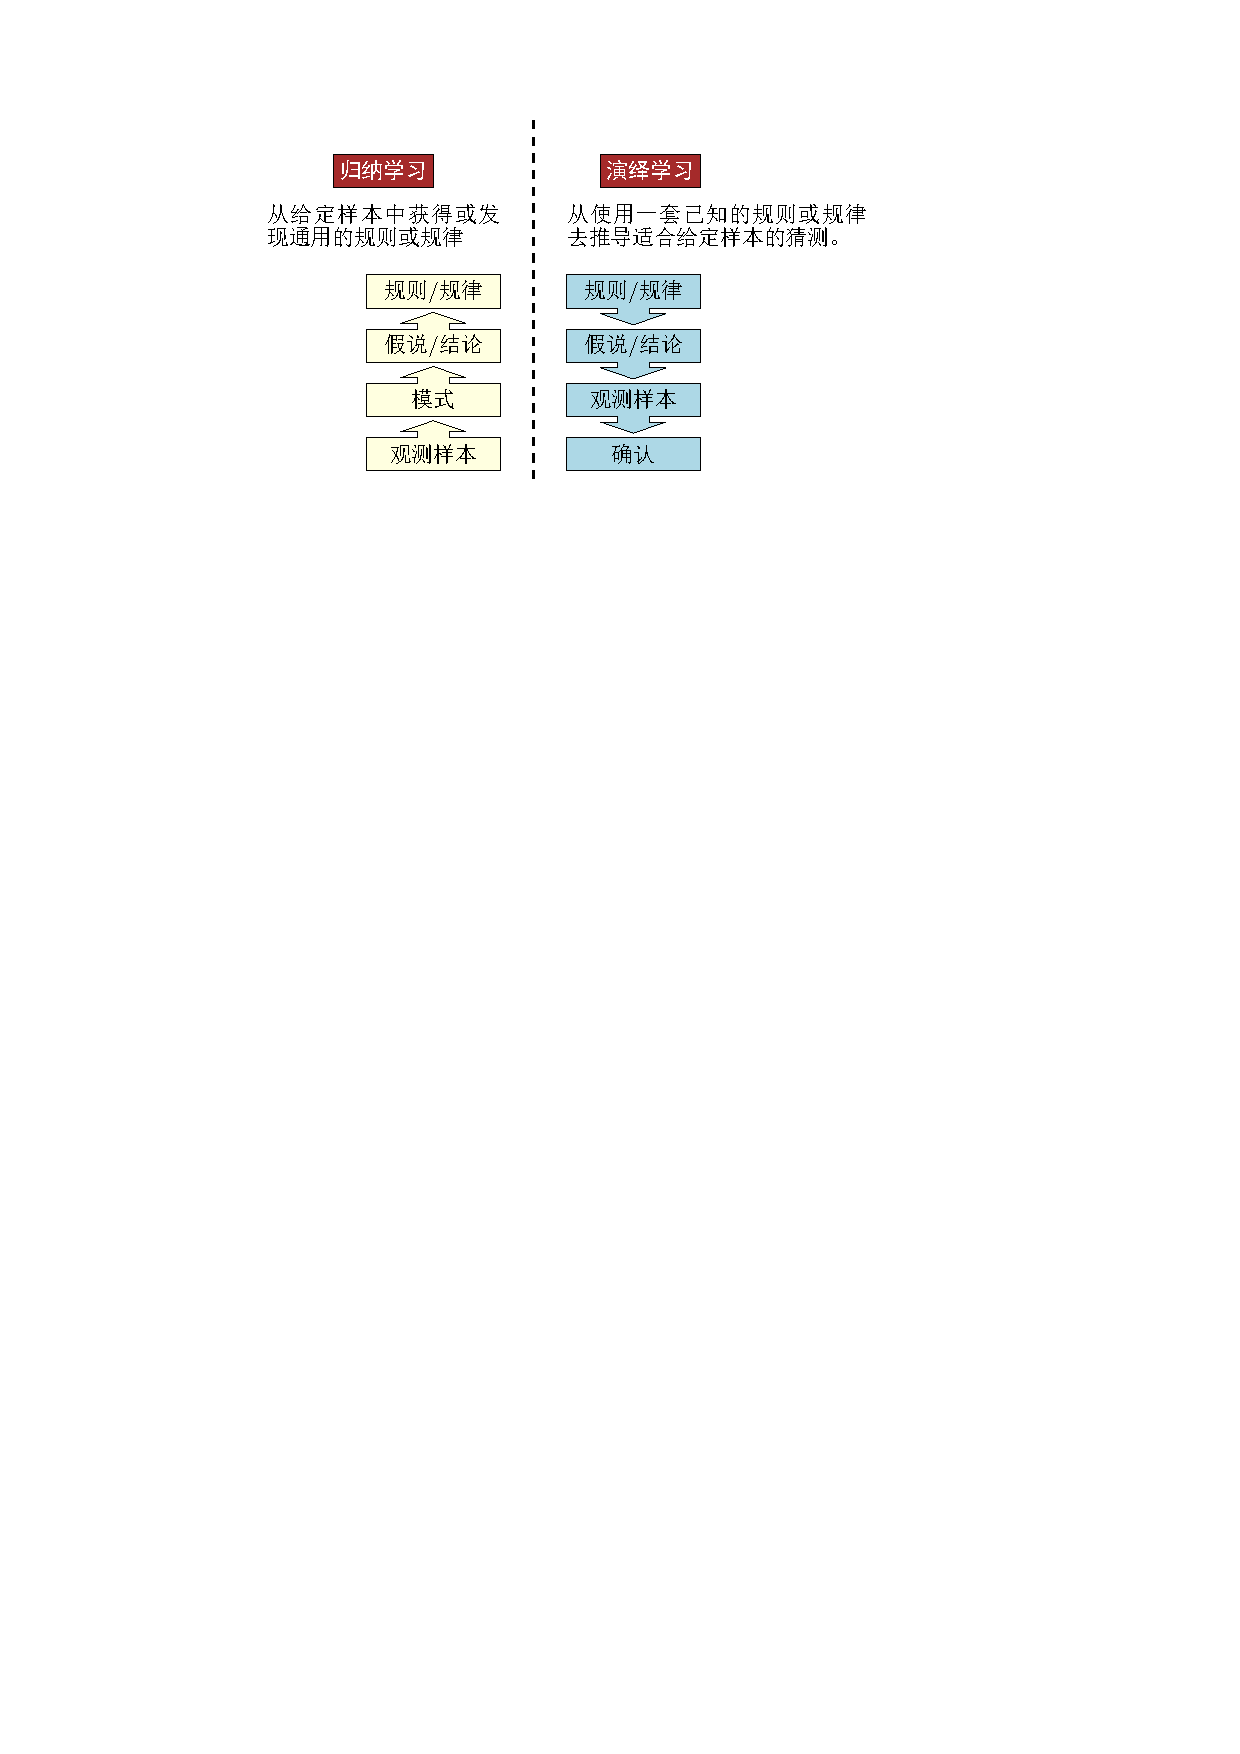
\includegraphics{image/两种通用的学习类型.pdf}
\end{figure}

\textcolor{main1}{机器学习思路}

\begin{itemize}
    \item 给定数据(样本、实例)和一定的学习规则,赋予机器自动从数据中获取知识的能力。
    \item 能够直接从样本(数据)中学习知识,不依赖于给定的判断规则。
    \item 机器学习的对象:计算机及互联网上的各种数字、文字、图像、视频、音频数据以及它们的组合。
    
    数据的基本假设是同类数据具有一定的统计规律性。
    \item 用于对数据(特别是未知数据)进行预测和分析。
\end{itemize}
\begin{figure}[htbp]
    \centering
    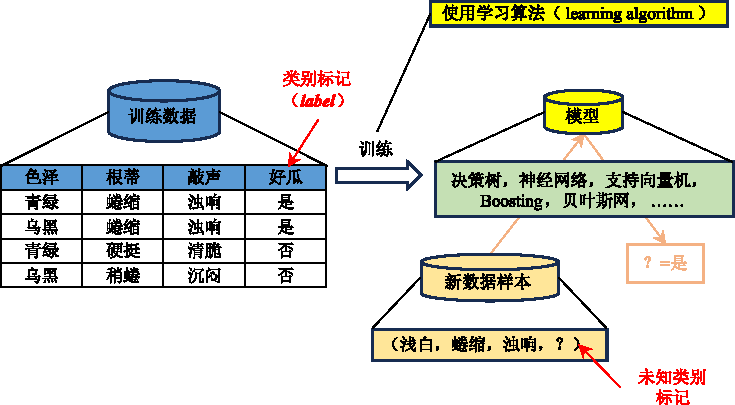
\includegraphics{image/机器学习思路.pdf}
\end{figure}
\begin{example}
    下列说法正确的是?
    \begin{enumerate}[A.]
        \item \textcolor{main1}{机器学习从数据中自动分析并获得规律}
        \item 机器学习中所采用的判断规则是事先给定的
        \item 利用已有公式可以计算的问题需要使用机器学习
        \item \textcolor{main1}{机器学习适于解决数据丰富且规则不明确的问题}
    \end{enumerate}
\end{example}
\textcolor{main1}{机器学习的数据}
\begin{itemize}
    \item \textcolor{main1}{样本:}关于一个对象或事件描述的一条记录
    \item \textcolor{main1}{特征(属性):}反映对象或事件在某方面的表现或性质
    \item \textcolor{main1}{标签:}样本标注的类别信息(离散)或者程度信息(连续),也可能没有。
\end{itemize}
\textcolor{main1}{归纳偏好}

机器学习算法在学习过程中对某种类型假设的偏好。
\begin{figure}[htbp]
    \centering
    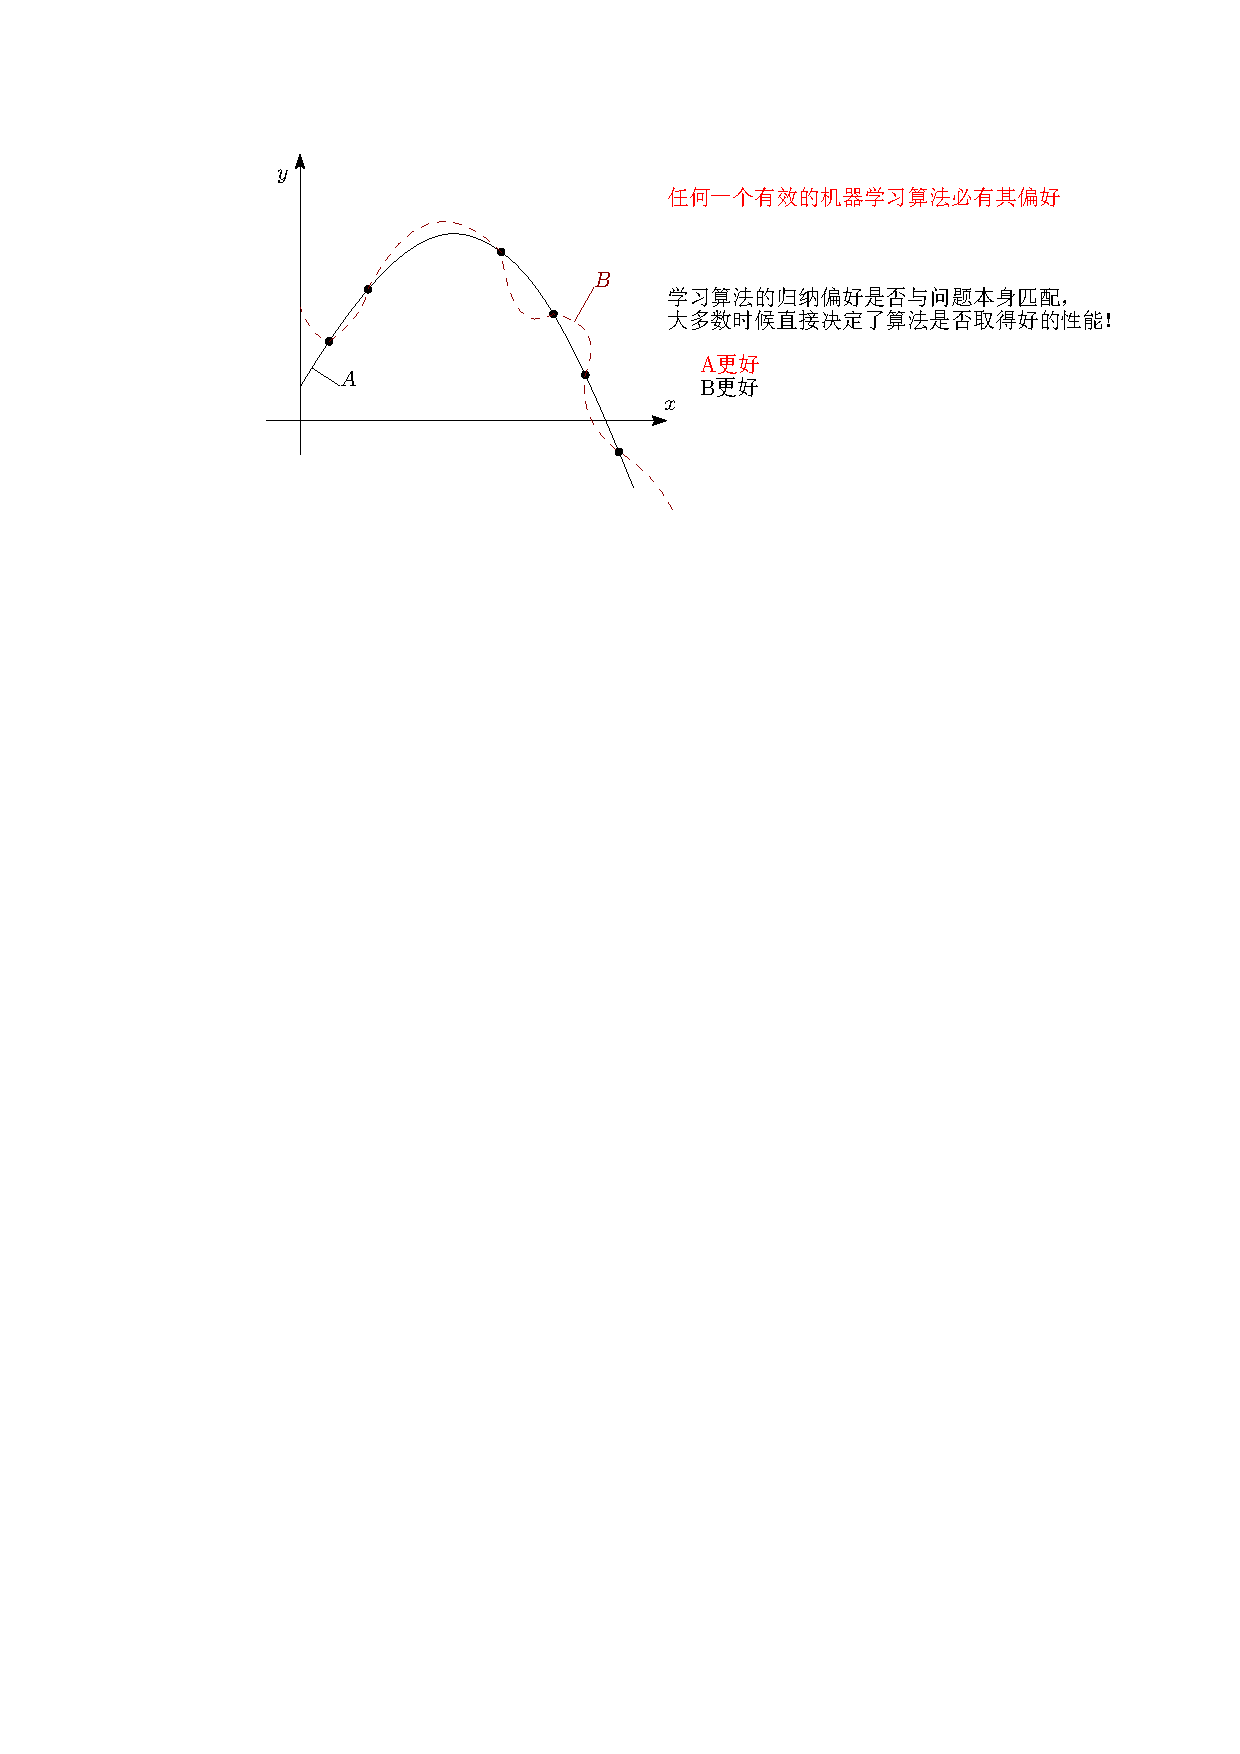
\includegraphics{image/归纳偏好.pdf}
\end{figure}

\textcolor{main1}{NFL(No Free Lunch)定理}

\begin{theorem}[NFL定理]
    一个算法A若在某些问题上比另一个算法B好,必存在另一些问题B比A好。
\end{theorem}
\begin{figure}[htbp]
    \centering
    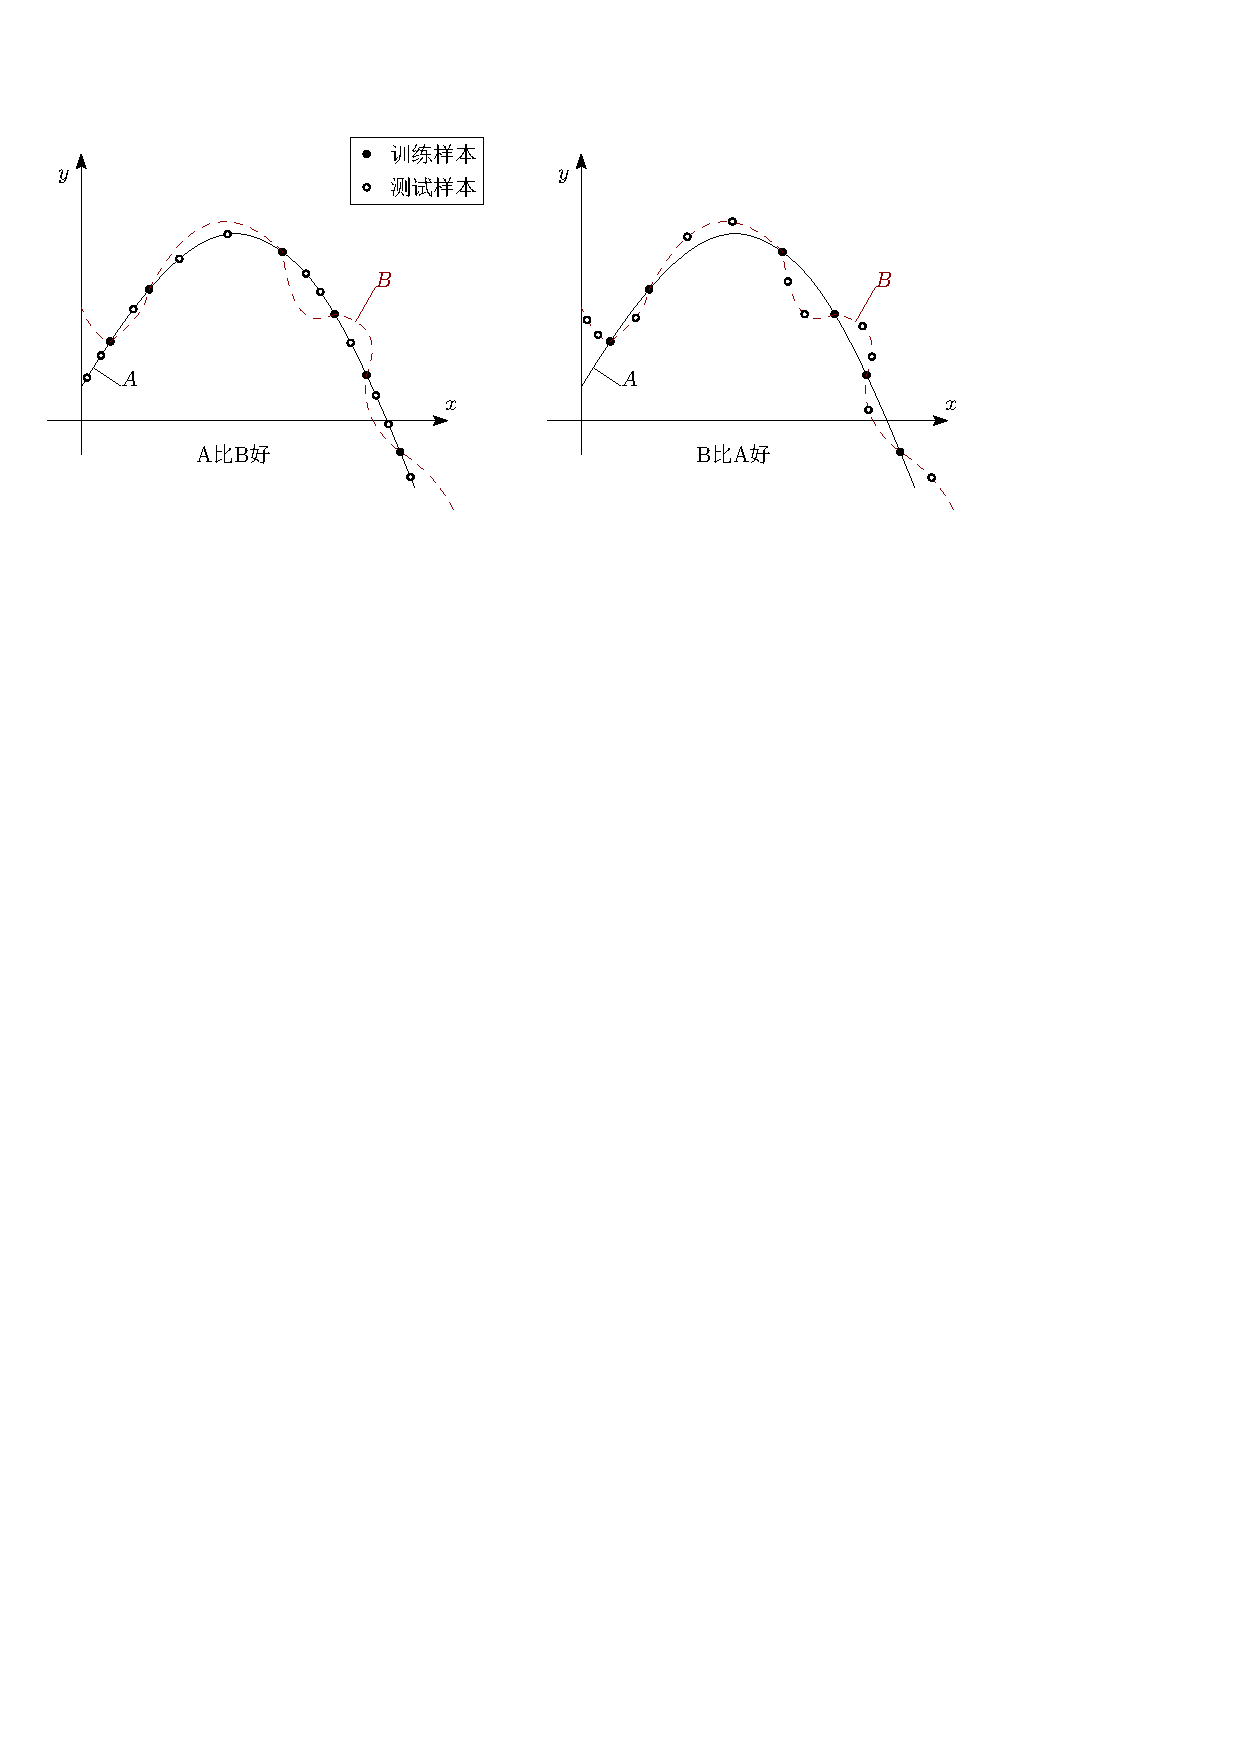
\includegraphics{image/NFL.pdf}
\end{figure}

\begin{definition}[泛化能力]
    机器学习的目标是使得学到的模型能很好的适用于“新样本”而不仅仅是训练集合,模型适用于新样本的能力被称为\textcolor{main1}{泛化(Generalization)能力}。
\end{definition}

\begin{figure}[htbp]
    \centering
    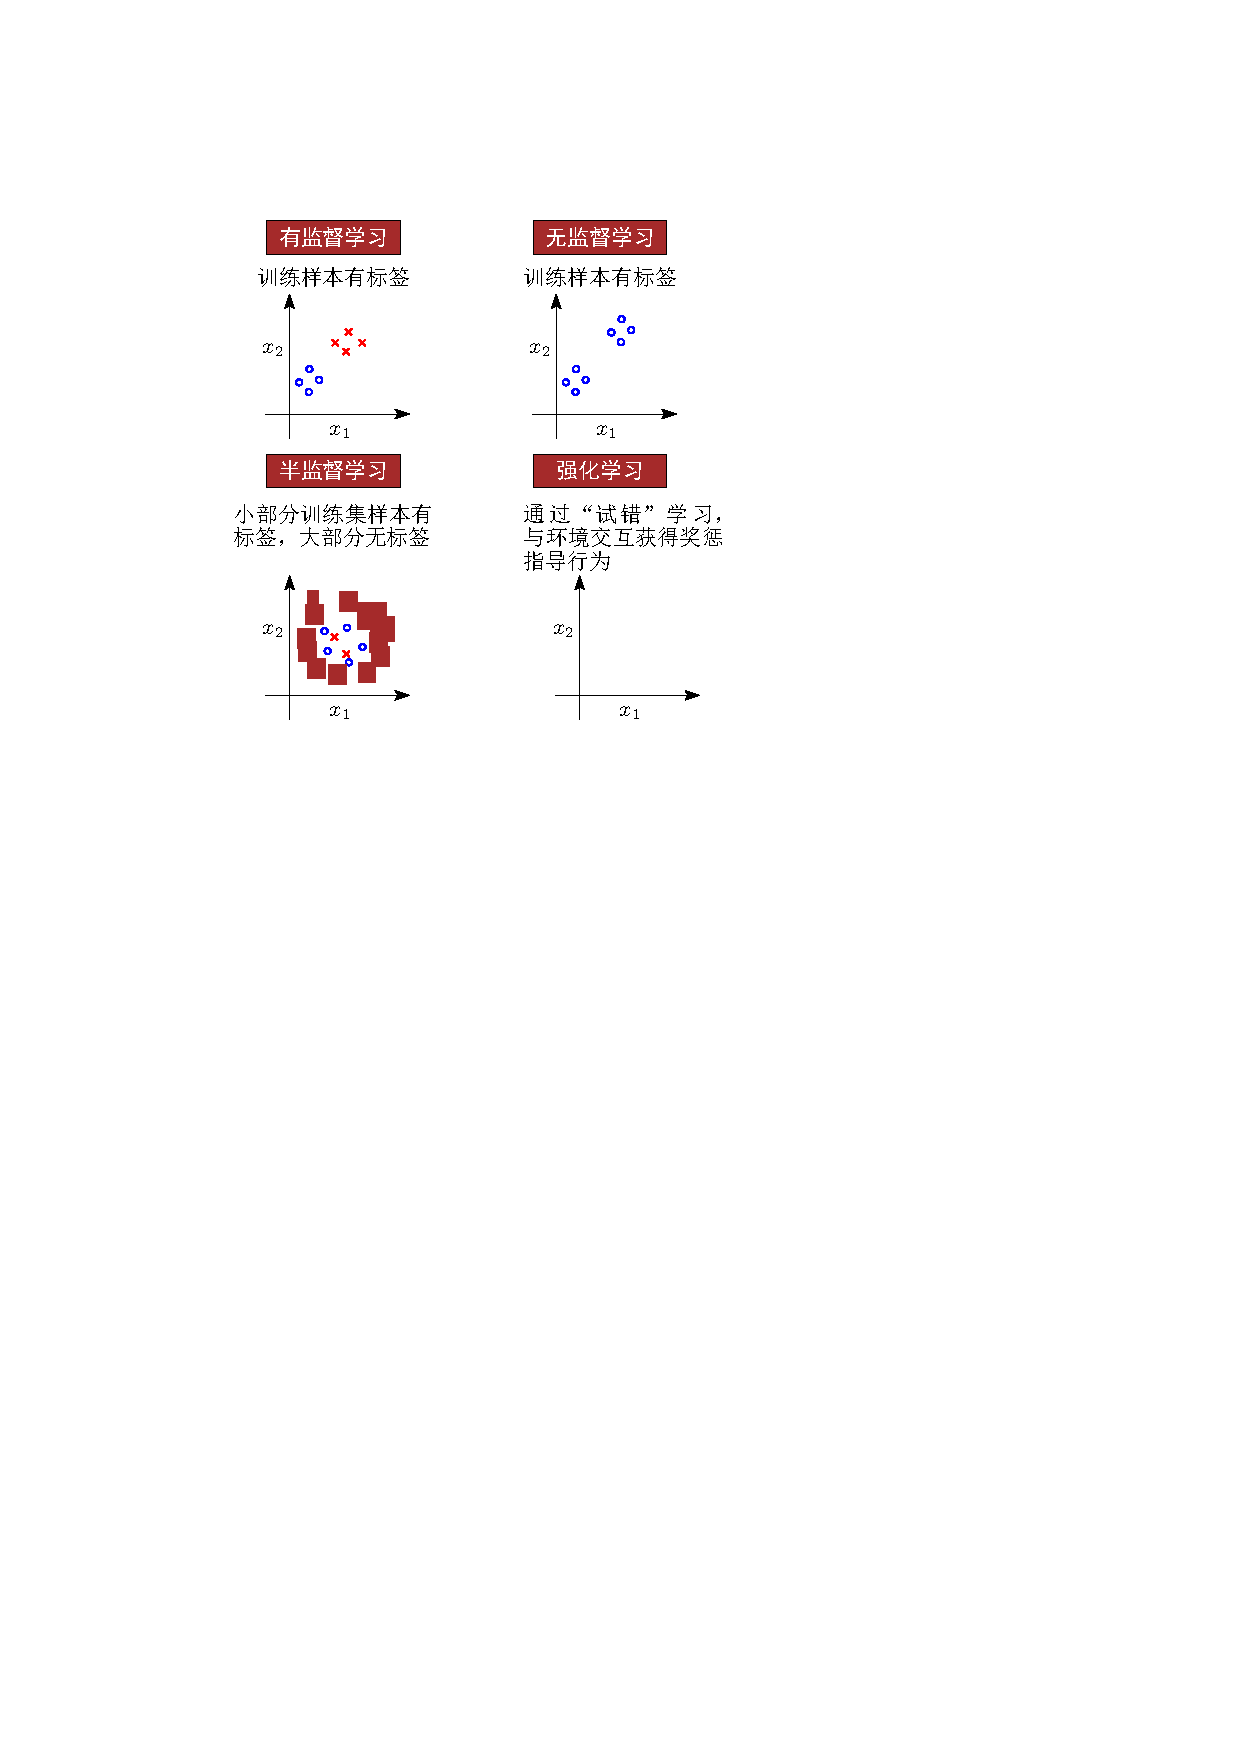
\includegraphics{image/机器学习的分类.pdf}
\end{figure}

\textcolor{main1}{强化学习vs. 有监督学习}
\begin{itemize}
    \item 相似点:
    \begin{enumerate}
        \item 强化学习中“状态”对应监督学习中的“示例”、“动作”对应“标签”,“策略”相当于“分类器”或“回归器”
        \item 强化学习中没有(监督学习中的那种)有标签样本(即“示例-标签”),换言之,没有人告诉机器在什么状态下应该做什么,而是通过最终结果“反思”之前的动作是否正确来进行学习
        \item 因此,强化学习在某种意义上可以看成具有“延迟标签信息”的监督学习问题
    \end{enumerate} 
    \item 不同点
    \begin{enumerate}
        \item 有监督学习的训练样本是有标签的,强化学习的训练是没有标签的,只有环境给出的奖惩
        \item 有监督学习的学习过程是静态的,不与环境进行交互,给什么样本就学什么。强化学习的学习过程是动态的,与环境进行交互,通过环境给出奖惩来学习。
        \item 有监督学习主要感觉感知问题,强化学习主要解决决策问题。
    \end{enumerate}
\end{itemize}
\begin{example}
    下面关于有监督学习说法正确的是?
    \begin{enumerate}[A]
        \item \textcolor{main1}{通过已知的训练样本来训练}
        \item \textcolor{main1}{训练样本是带有标签的}
        \item 对于训练集之外的样本,学习到的模型不能够预测结果
        \item \textcolor{main1}{可以应用于目标识别中}
    \end{enumerate}
\end{example}
\subsection{有监督学习基本方法}
回归和分类取决于训练用的标签是连续还是离散的,它们预测获得标签也对应的是连续和离散的。

\textcolor{main1}{有监督学习的一般过程}
\begin{itemize}
    \item 数据准备
    \begin{itemize}
        \item 如果问题是全新的 ,采集或爬取带标签的数据;如果数据仓库有相应的数据,将数据提取出来。
        \item 数据准备好之后,需要对数据进行预处理,主要包括重复数据检测、数据标准化、数据编码、缺失值处理、异常值处理等。
    \end{itemize}
    \item 特征选择或抽取
    \begin{itemize}
        \item 特征选择:选取原始特征集合的有效子集,保留有用特征,移除冗余或无关的特征。
        \item 特征抽取:构造一个新的特征空间,将原始特征投影到新的空间中表示。
    \end{itemize}
    \item 训练——从数据中学习获得模型的过程,包括选择模型和确定参数。
    \begin{itemize}
        \item 超参数,如深度学习模型中各层的神经元数量;
        \item 模型内部参数,如深度学习模型中神经元间的连接权值。
    \end{itemize}
    \item 验证/测试——选取一部分已知类别的样本评估模型分类效果
    \begin{itemize}
        \item 误差:模型输出与真值的偏离程度
        \item 训练 (经验) 误差:模型在训练集上的误差
        \item 测试误差:模型在测试集上的误差
        \item 泛化误差:在除训练集外所有样本上的误差
    \end{itemize}
    \begin{note}
        验证/测试的注意:
        \begin{itemize}
            \item 假设测试集是从样本真实分布中独立采样获得,将测试集上的“测试误差”作为泛化误差的近似,所以测试集要和训练集中的样本互斥。
            \item 独立测试集:选择与训练样本相独立的数据集进行验证,评估模型的分类效果。
            \item 交叉验证:将原始数据分组,大部分作为训练集,进行训练模型;另一部分作为验证集,测试训练得到的模型的正确率,用来调整模型参数。k 折交叉验证是将原始数据分为k 组,每次留1 组作为验证集。特例:留1 法。
        \end{itemize}
    \end{note}
    \item K折交叉验证(K-fold cross-validation)
    \begin{figure}[htbp]
        \centering
        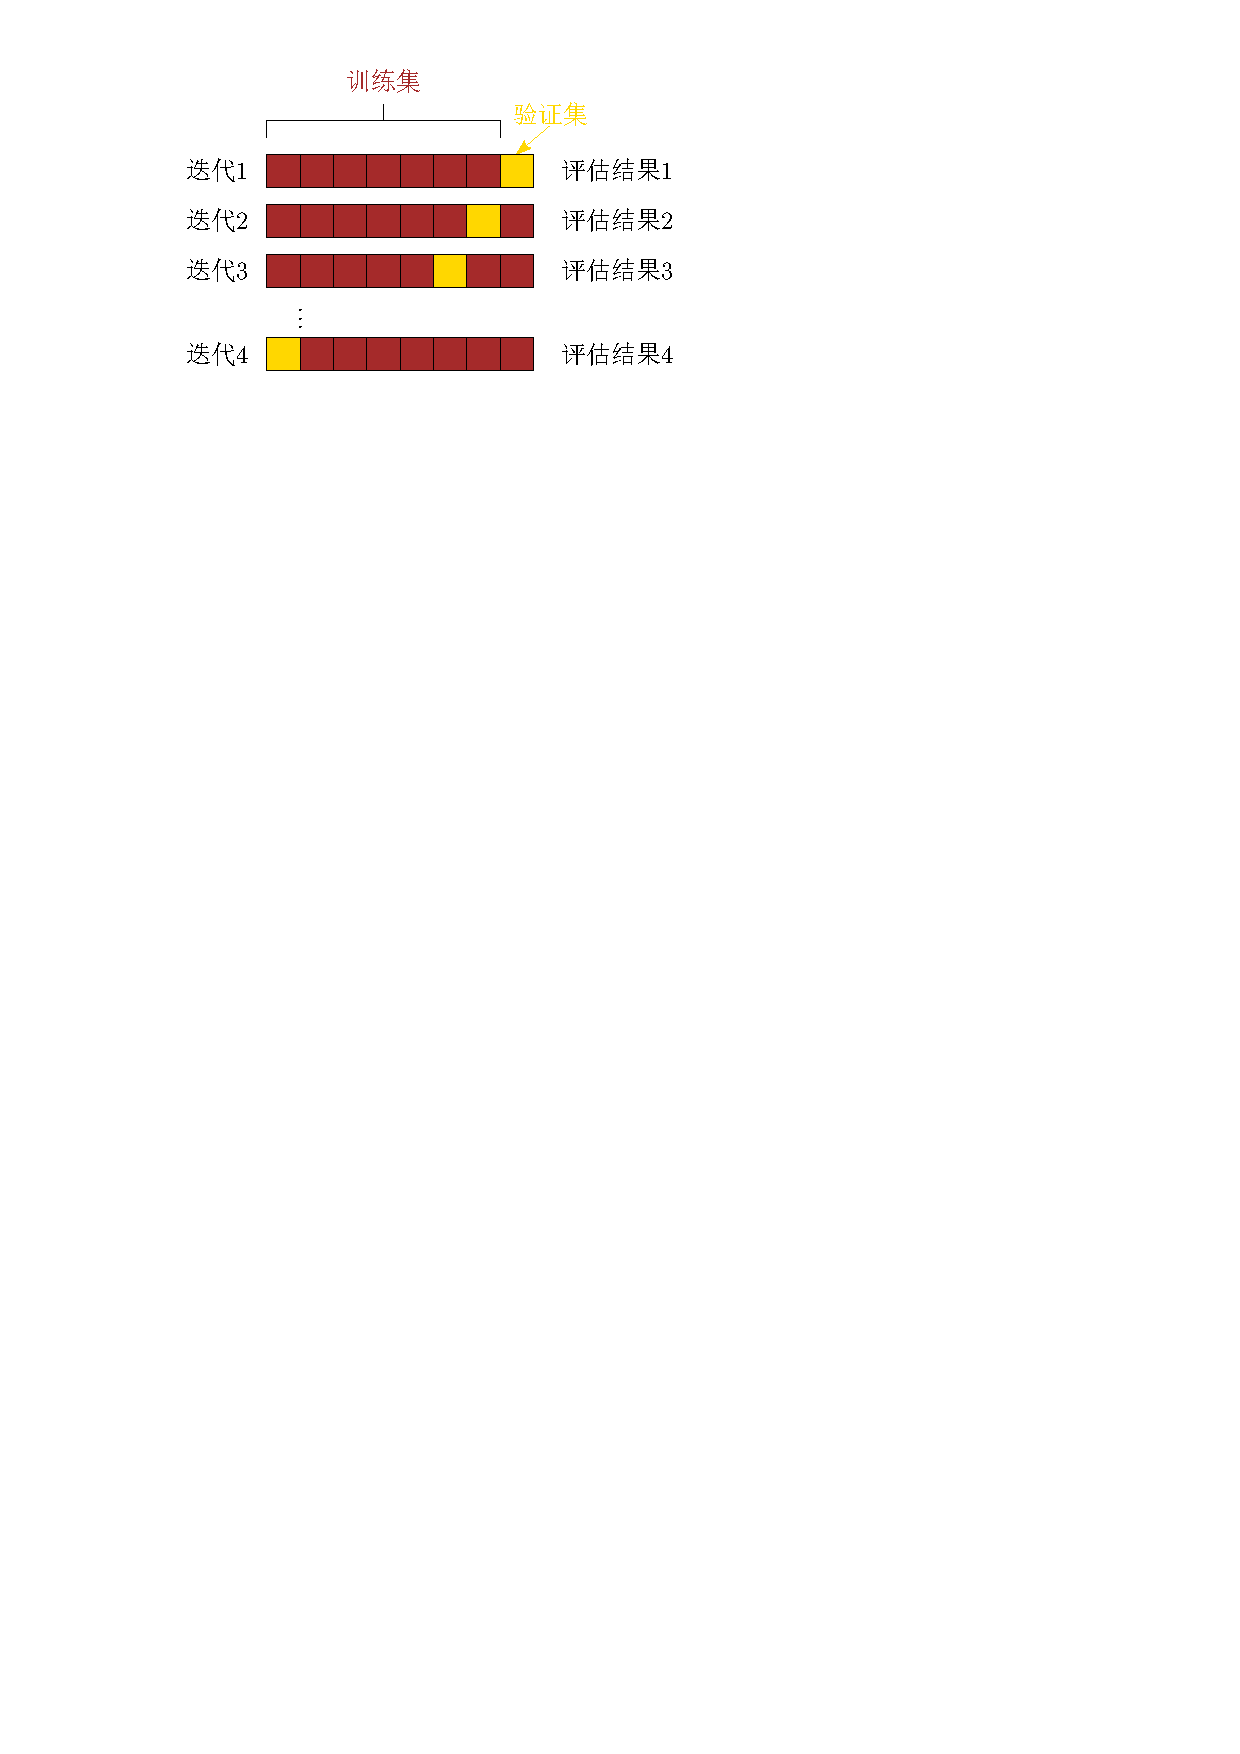
\includegraphics{image/K折交叉验证.pdf}
    \end{figure}
    \begin{itemize}
        \item 初始采样分割成K个子样本,一个单独的子样本被保留作为验证模型的数据,其他K-1个样本用来训练。
        \item 交叉验证重复K次,每个子样本验证一次,最终得到一个单一估测。
        \item 这个方法的优势在于,同时重复运用随机产生的子样本进行训练和验证,每次的结果验证一次,10折交叉验证是最常用的。
    \end{itemize}
\end{itemize}
\begin{example}
    思考题:
    \begin{enumerate}
        \item 训练数据、验证数据可以有交叠吗?
        
        不能有交叠。
        \item 为什么要进行交叉验证,随机选取其中一部分只做一次测试好不好?
        
        多次交叉验证的效果更好,可以充分利用已知数据计算出多个预测正确率,获得最终预测正确率的平均值和方差,更准确地评估模型的预测效果。
    \end{enumerate}
\end{example}
\begin{example}
    影响有监督学习性能的因素有哪些?
    \begin{enumerate}[A]
        \item \textcolor{main1}{可用数据的样本规模}
        \item \textcolor{main1}{数据预处理}
        \item \textcolor{main1}{特征抽取与选择}
        \item \textcolor{main1}{机器学习算法设计}
    \end{enumerate}
\end{example}
\subsubsection{回归问题}
\textcolor{main1}{最小二乘法}

回归方程:$\hat{y} = f(x) = \boldsymbol{x}^{\mathrm{T}}\boldsymbol{w} + b$

\[
    \begin{array}{ll}
        (\boldsymbol{w}^{*},b^{*}) &= \arg\min\limits_{(\boldsymbol{w},b)}\sum_{i = 1}^{m}\left( f(x_i)-y_i \right)^2\\
        &= \arg\min\limits_{(\boldsymbol{w},b)}\sum_{i = 1}^{m}\left( y_i - \boldsymbol{x}_i^{\mathrm{T}}\boldsymbol{w} - b \right)^2
    \end{array}
\]
\[
    Q = \sum_{i = 1}^{m}\left( y_i - \boldsymbol{w}^{\mathrm{T}}\boldsymbol{x}_i - b \right)^2 = (\boldsymbol{y}-\boldsymbol{X}\hat{\boldsymbol{w}})^{\mathrm{T}} (\boldsymbol{y}-\boldsymbol{X}\hat{\boldsymbol{w}})
\]
其中,$\boldsymbol{X}$和$\hat{\boldsymbol{w}}$为
\[
    \boldsymbol{X} = \begin{bmatrix}
        \boldsymbol{x}_1^{\mathrm{T}} & 1\\
        \vdots & \vdots \\
        \boldsymbol{x}_m^{\mathrm{T}} & 1\\
    \end{bmatrix},\,
    \hat{\boldsymbol{w}} = \begin{bmatrix}
        \boldsymbol{w}\\
        b
    \end{bmatrix} 
\]
求其偏导数并令其为$\boldsymbol{0}$,即:
\[
    \begin{array}{c}
        \dfrac{\partial Q}{\partial \hat{\boldsymbol{w}}} = 2\boldsymbol{X}^{\mathrm{T}}\boldsymbol{Xw}-2\boldsymbol{X}^{\mathrm{T}}\boldsymbol{y} = \boldsymbol{0}\\
        \hat{\boldsymbol{w}} = \left( \boldsymbol{X}^{\mathrm{T}}\boldsymbol{X} \right)^{-1}\boldsymbol{X}^{\mathrm{T}}\boldsymbol{y}
    \end{array}
\]

\begin{example}
    \textcolor{main1}{改进线性回归问题性能的方法包括}
    \begin{enumerate}[A]
        \item \textcolor{main1}{引入新的特征}
        \item \textcolor{main1}{提高多项式模
        型的阶次}
        \item \textcolor{main1}{选择合适的曲线回归模型}
        \item \textcolor{main1}{抽取更有效的特征}
    \end{enumerate}
\end{example}

\textcolor{main1}{非线性回归}
\begin{definition}[非线性回归]
    两种回归通过在目标函数中引入\textcolor{main1}{正则化项}来处理\textcolor{main1}{多重共线性问题},并达到防止过拟合的目的。岭回归采用的是L2正则化,
而Lasso回归采用的是L1正则化。    
\end{definition}
\begin{figure}[htbp]
    \centering
    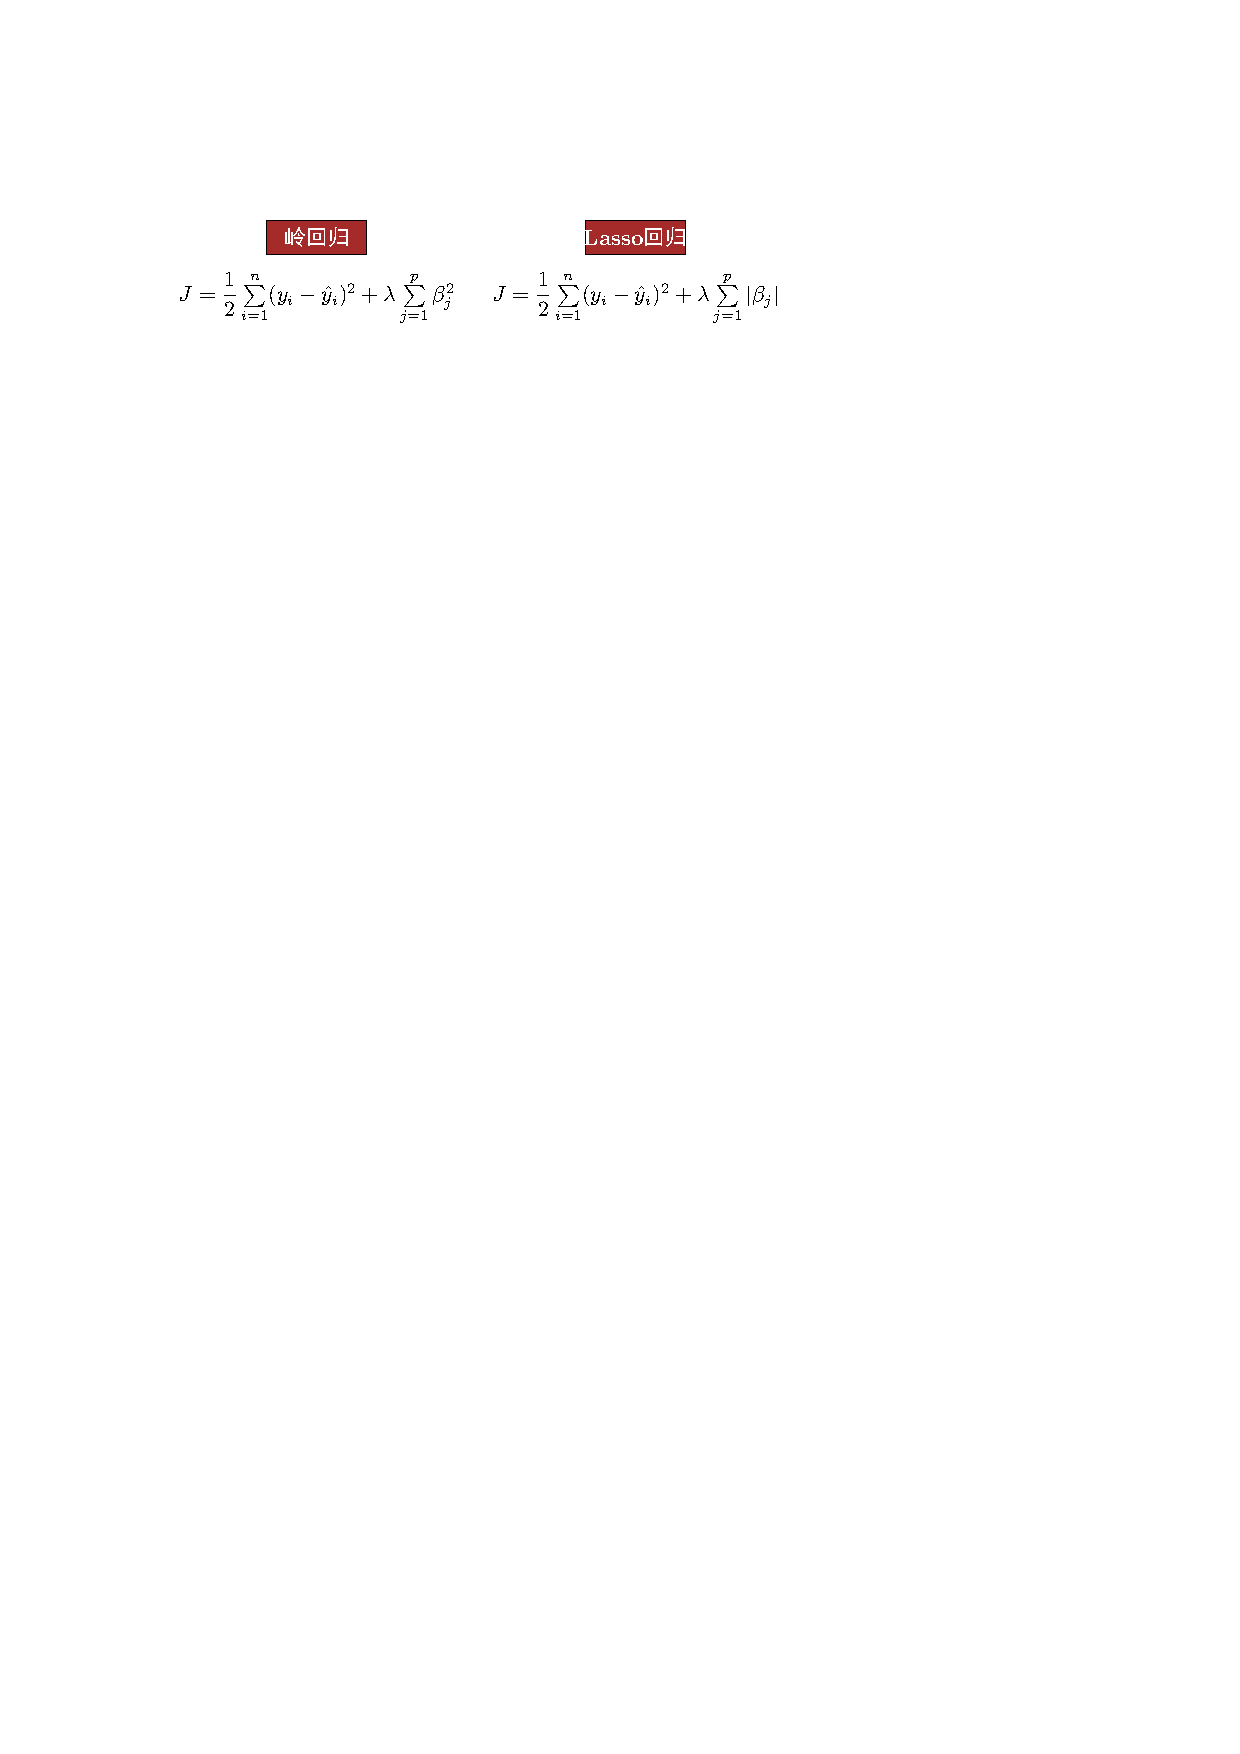
\includegraphics{image/非线性回归.pdf}
\end{figure}

\subsubsection{分类问题}
\begin{definition}[分类问题]
    分类也是有监督学习的一种。它解决的是样本的标签是离散值的情况,其试图给出的预测值也是离散的。
    \begin{itemize}
        \item \textcolor{main1}{二分类问题:}非此即彼的分类问题,输出值,0或1,0代表不合格,1代表合格
        \item \textcolor{main1}{多分类问题:}如分四等次,对应预测离散输出值为0、1、2、3。0代表不及格、1表示及格、2表示良好、3表示优秀。
    \end{itemize}
\end{definition}

\begin{example}
    能否将分类问题的标签作为输出值直接利用回归算法求解?
    \begin{enumerate}[A]
        \item 能
        \item \textcolor{main1}{不能}
    \end{enumerate}
\end{example}

\textcolor{main1}{分类问题性能度量}

衡量模型泛化能力的评价标准,反映了任务需求,使用不同的性能度量往往会导致不同的评判结果。
\begin{itemize}
    \item  在对于分类任务,错误率和准确率是最常用的两种性能度量:
    \begin{itemize}
        \item 分类错误率:分错样本占样本总数的比例
        \[
            E(f;D) = \dfrac{1}{m}\sum_{i = 1}^{m}I_{f(x_i)\neq y_i}
        \]
        \item 分类准确率:分对样本占样本总数的比例
        \[
            acc(f;D) = \dfrac{1}{m}\sum_{i = 1}^{m}I_{f(x_i)= y_i} = 1-E(f;D)
        \]
        \item 诊断、检测等应用场景中,查准率和查全率比分类错误率和分类精度更适合。
        \begin{figure}[htbp]
            \centering
            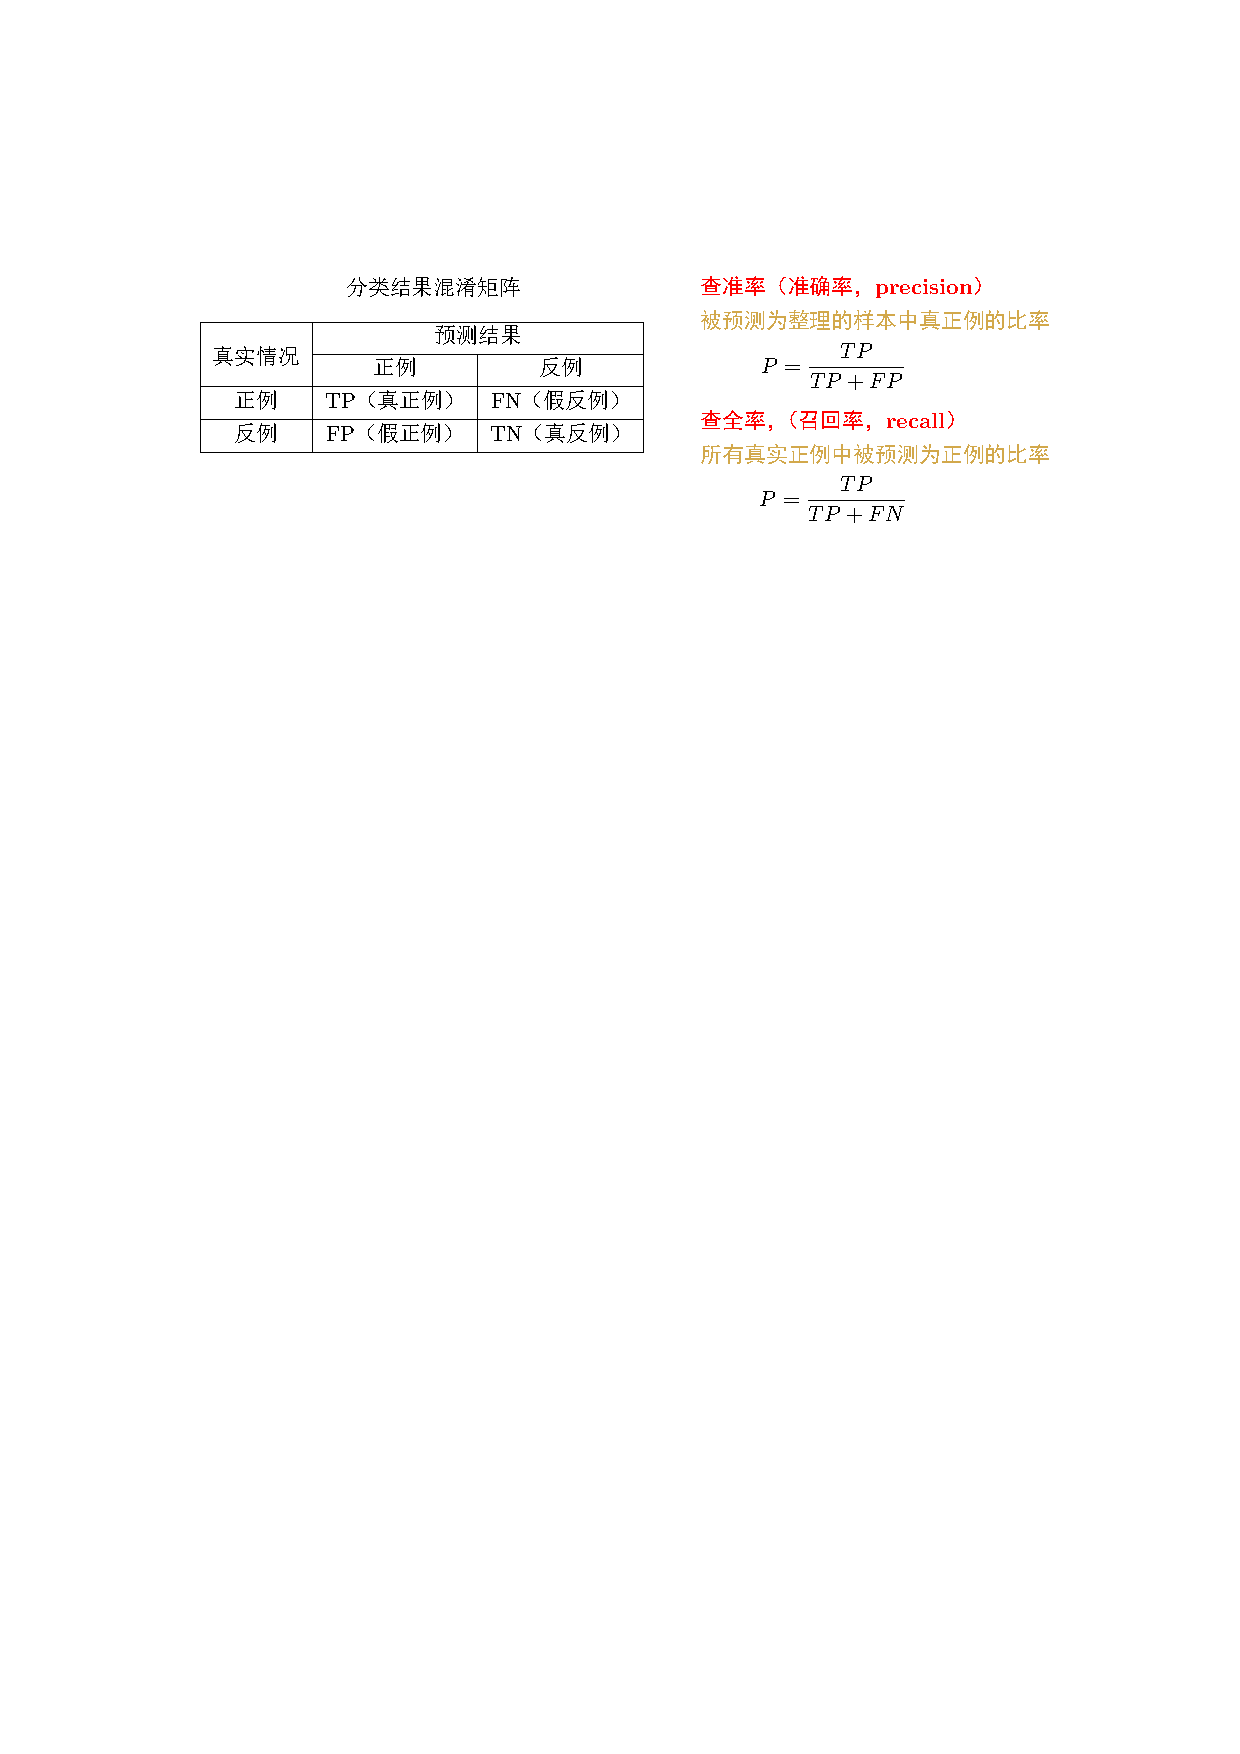
\includegraphics{image/混淆矩阵.pdf}
        \end{figure}

        查准率和查全率是一对矛盾的度量。
    \end{itemize}
\end{itemize}

\textcolor{main1}{线性判别分析}
\begin{figure}[htbp]
    \centering
    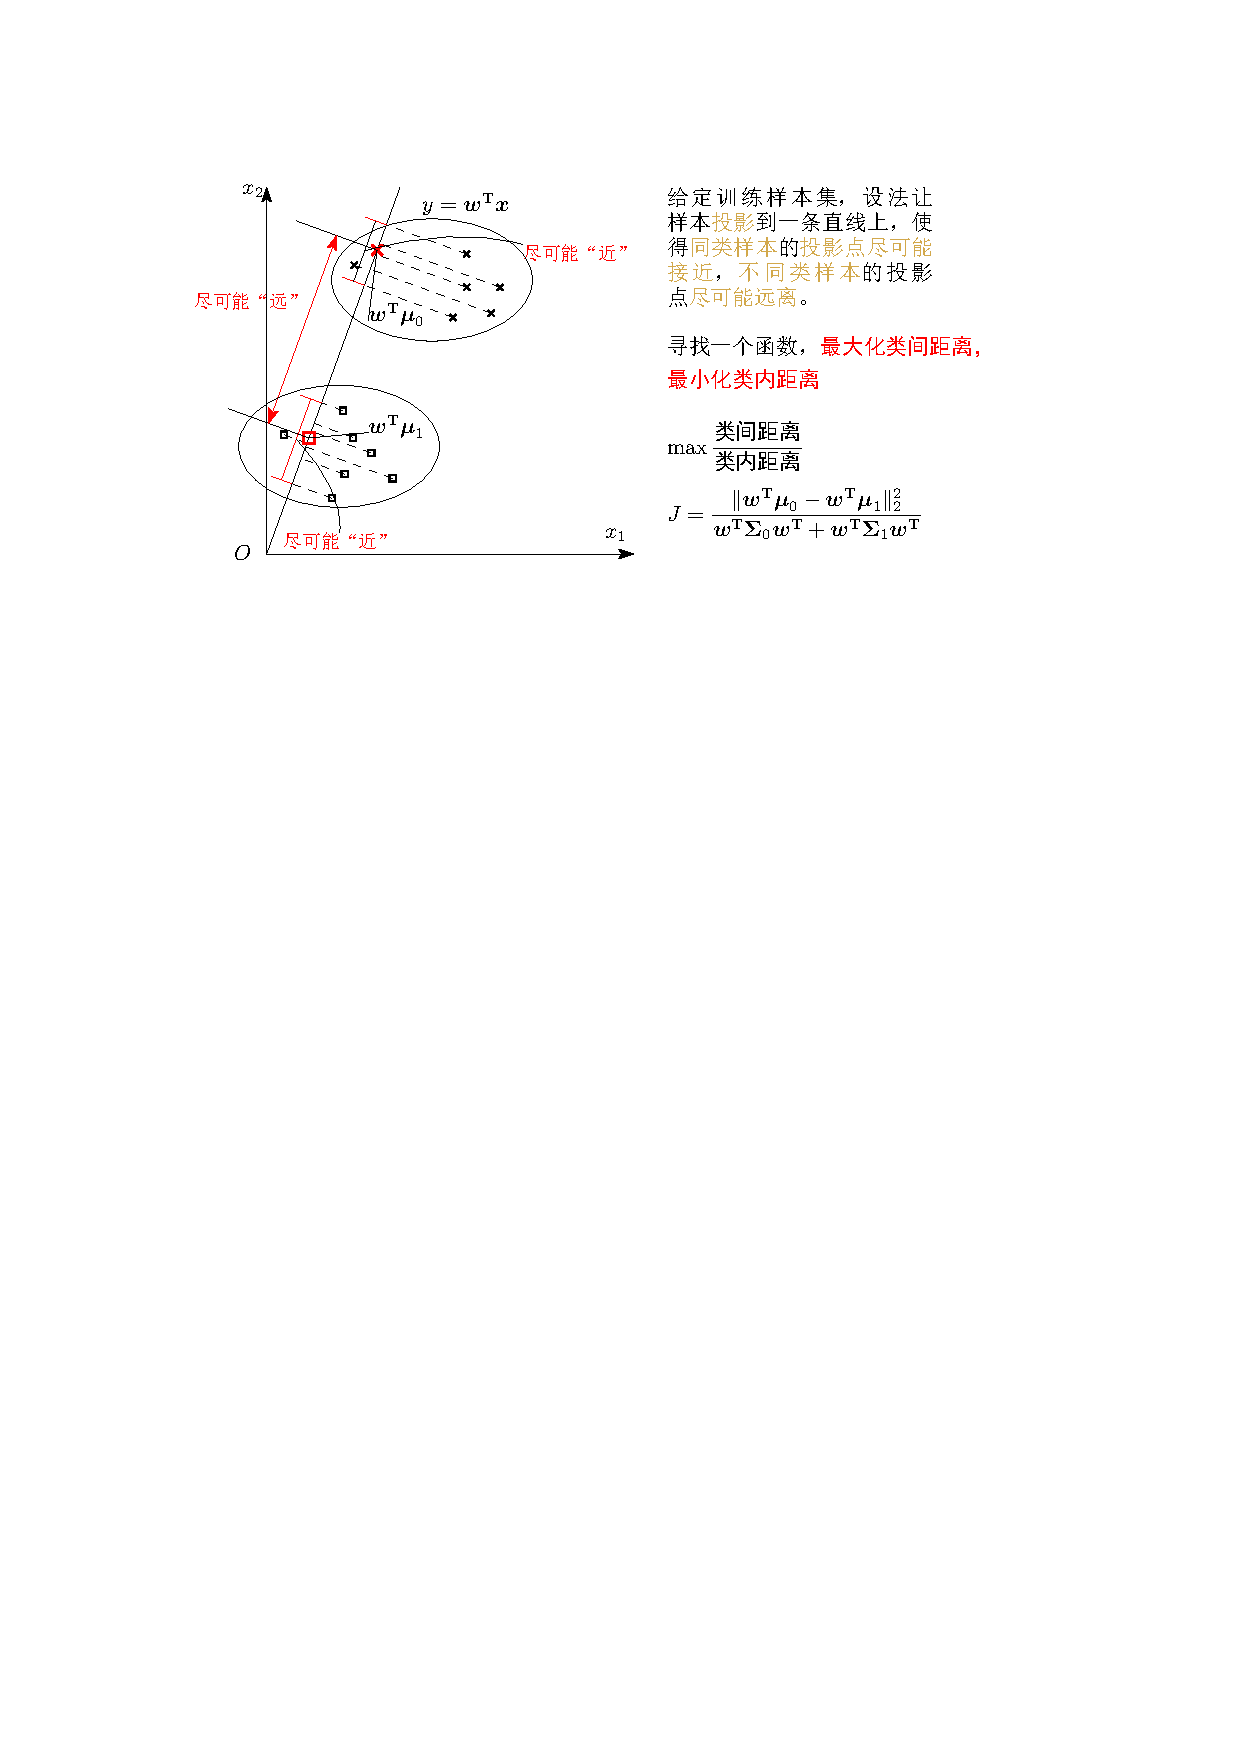
\includegraphics{image/线性判别分析.pdf}
\end{figure}
\[
    \begin{array}{ll}
        J &= \dfrac{\| \boldsymbol{w}^{\mathrm{T}}\boldsymbol{\mu}_0 - \boldsymbol{w}^{\mathrm{T}}\boldsymbol{\mu}_1 \|_2^2}{ \boldsymbol{w}^{\mathrm{T}}\boldsymbol{\Sigma}_0\boldsymbol{w}^{\mathrm{T}} + \boldsymbol{w}^{\mathrm{T}}\boldsymbol{\Sigma}_1\boldsymbol{w}^{\mathrm{T}} }\\
        &=\dfrac{\boldsymbol{w}^{\mathrm{T}}\left( \boldsymbol{\mu}_0-\boldsymbol{\mu}_1 \right)\left( \boldsymbol{\mu}_0-\boldsymbol{\mu}_1 \right)^{\mathrm{T}}\boldsymbol{w}}{ \boldsymbol{w}^{\mathrm{T}}\left( \boldsymbol{\Sigma}_0 + \boldsymbol{\Sigma}_1 \right)\boldsymbol{w}}
    \end{array}
\]
记$\boldsymbol{S}_{b} \overset{\triangle}{=}\left( \boldsymbol{\mu}_0-\boldsymbol{\mu}_1 \right)\left( \boldsymbol{\mu}_0-\boldsymbol{\mu}_1 \right)^{\mathrm{T}},\, \boldsymbol{S}_{w} \overset{\triangle}{=}\boldsymbol{\Sigma}_0 + \boldsymbol{\Sigma}_1$
那么
\[
    J = \dfrac{\boldsymbol{w}^{\mathrm{T}}\boldsymbol{S}_{b}\boldsymbol{w}}{ \boldsymbol{w}^{\mathrm{T}}\boldsymbol{S}_{w}\boldsymbol{w}}
\]
令$ \boldsymbol{w}^{\mathrm{T}}\boldsymbol{S}_{w}\boldsymbol{w} = 1$,最大化广义瑞利商等价形式为
\[
    \begin{array}{c}
        \min\limits_{\boldsymbol{w}} -\boldsymbol{w}^{\mathrm{T}}\boldsymbol{S}_{b}\boldsymbol{w}\\
        \operatorname{s.t.} \boldsymbol{w}^{\mathrm{T}}\boldsymbol{S}_{w}\boldsymbol{w} = 1
    \end{array}
\]
\textcolor{main1}{由拉格朗日乘子法可得}
\[
    \boldsymbol{S}_b\boldsymbol{w} = \lambda\boldsymbol{S}_{w}\boldsymbol{w}\rightarrow \boldsymbol{w} = \boldsymbol{S}_{w}^{-1}\left( \boldsymbol{\mu}_0-\mu_{1} \right)    
\]
两类数据同先验、满足高斯分布且协方差相等时,线性判别分析达到最优分类。
\begin{example}
    现有两类样本,请计算其线性判别分类器。
    \begin{itemize}
        \item 第1类:
        \[
            \boldsymbol{X}_1 = \left\{ (4,2),\,(2,4),\,(2,3),\,(3,6),\,(4,4) \right\}
        \]
        \item 第2类:
        \[
            \boldsymbol{X}_2 = \left\{ (9,10),\,(6,8),\,(9,5),\,(8,7),\,(10,8) \right\}
        \]
    \end{itemize}
    均值向量:
    \[
        \boldsymbol{\mu}_1 = \begin{bmatrix}
            3 & 3.8
        \end{bmatrix}^{\mathrm{T}},\,\boldsymbol{\mu}_2 = \begin{bmatrix}
            8.4 & 7.6
        \end{bmatrix}^{\mathrm{T}}
    \]
    散度矩阵:
    \[
        \boldsymbol{\Sigma}_1 = \begin{bmatrix}
            1   & -0.25 \\
            -0.25 & 2.2
        \end{bmatrix},\,\boldsymbol{\Sigma}_2 = \begin{bmatrix}
            2.3 & -0.05 \\
            -0.05 & 3.3
        \end{bmatrix}
    \]
    类内散度:
    \[
        \boldsymbol{S}_{w} = \boldsymbol{\Sigma}_1 + \boldsymbol{\Sigma}_2 = \begin{bmatrix}
            3.3 & -0.3 \\
            -0.3 & 5.5 \\
        \end{bmatrix}
    \]
    $\boldsymbol{S}_{w}$的逆
    \[
        \boldsymbol{S}_{w}^{-1} = \begin{bmatrix}
            0.30454 & 0.016611 \\
            0.016611 & 0.182724 \\
        \end{bmatrix}
    \]
    故而$\boldsymbol{w}$为
    \[
        \boldsymbol{w} = \boldsymbol{S}_{w}^{-1}\left( \boldsymbol{\mu}_0-\boldsymbol{\mu}_1 \right) = \begin{bmatrix}   
            -1.70764 & -0.78405
        \end{bmatrix}^{\mathrm{T}}
    \]
\end{example}

\textcolor{main1}{支持向量机}

\begin{figure}[htbp]
    \centering
    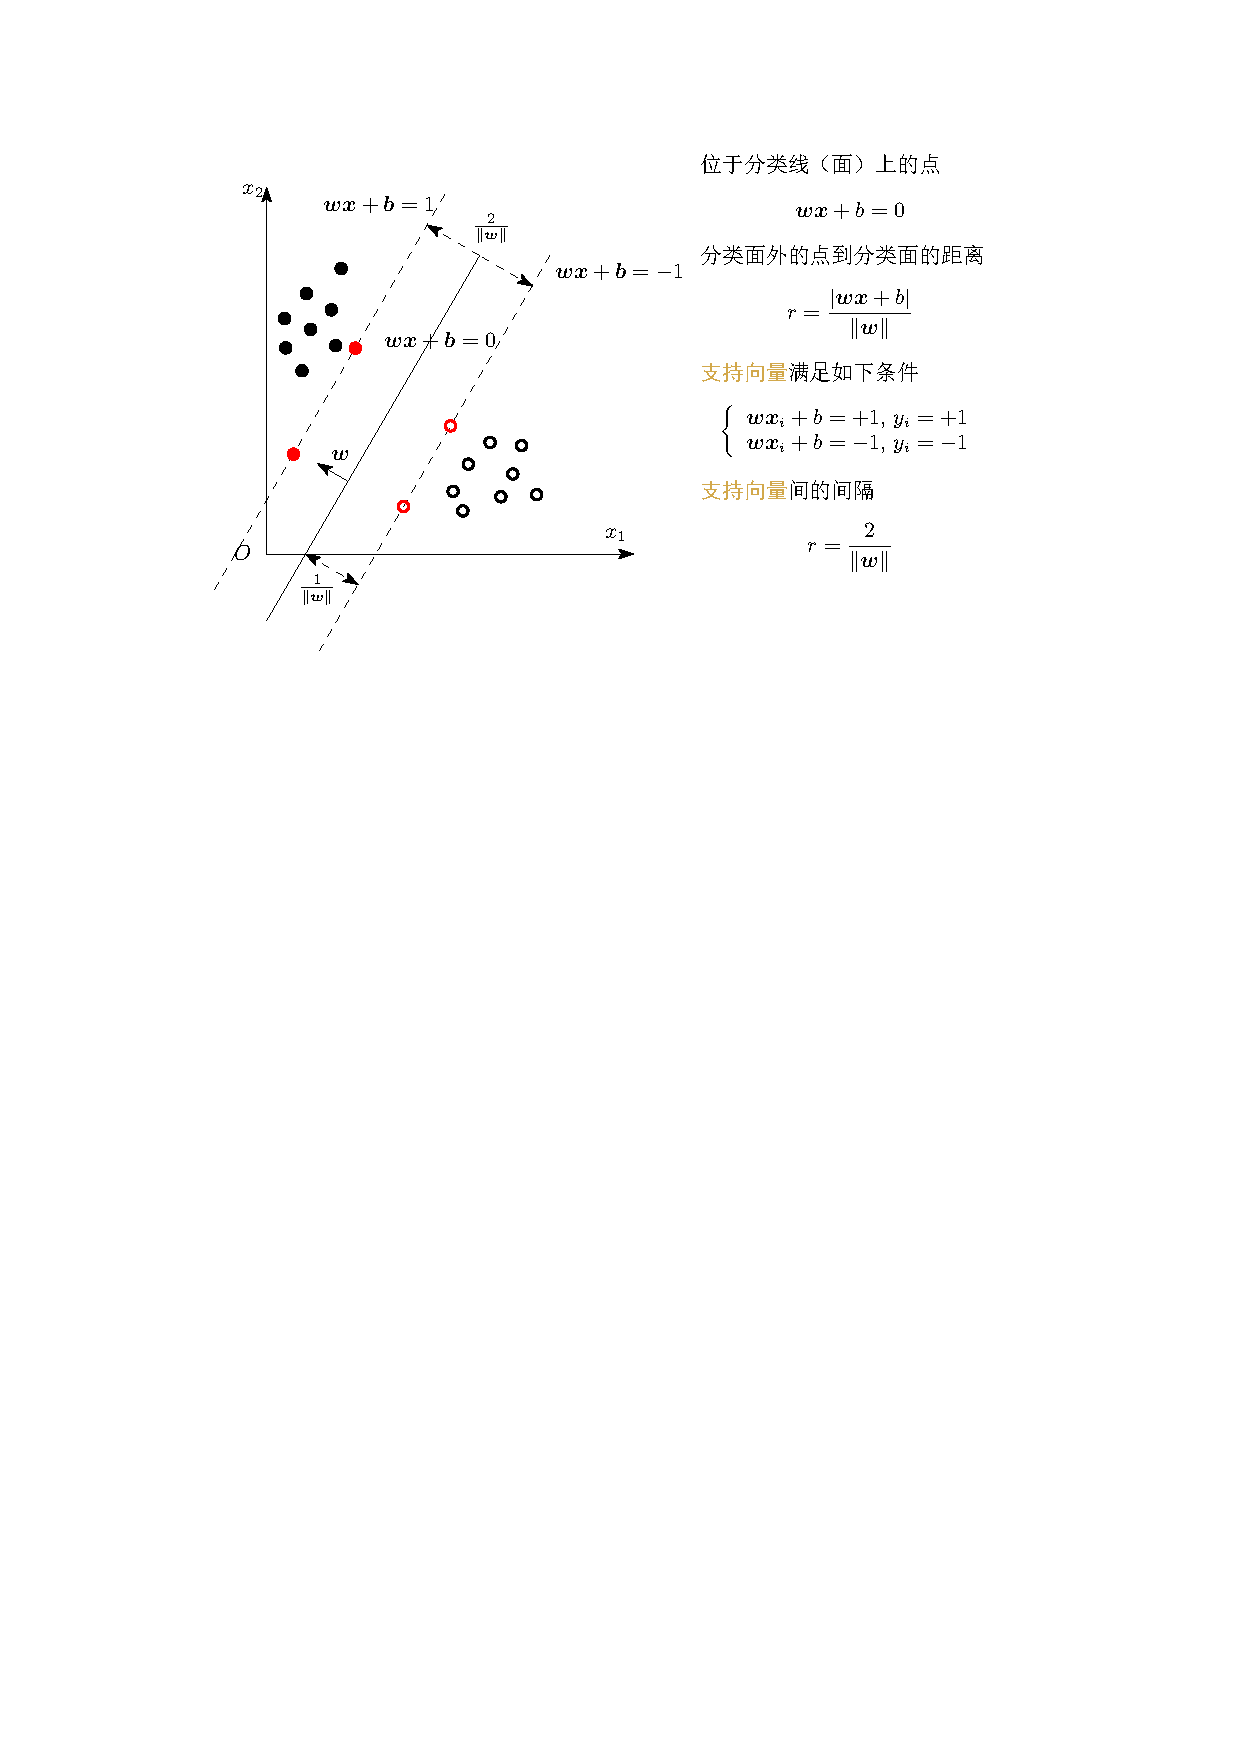
\includegraphics{image/支持向量机.pdf}
\end{figure}
\textcolor{main1}{最大间隔原则:}

选择参数对$(\boldsymbol{w},b)$使得训练集对于线性函数$\boldsymbol{wx}+b = 0$的几何间隔取最大值,构造决策函数
\[
    \begin{array}{l}
        \min\limits_{\boldsymbol{w},b} \dfrac{1}{2}\|\boldsymbol{w}\|^2\\
        \operatorname{s.t.}\, y_i\left( \boldsymbol{wx}_i+b \right)\geq 1
    \end{array}
\]
为求解上述问题,使用使用Lagrange乘子法将其转化为对偶问题。于是引入Lagrange函数:
\[
    L\left( \boldsymbol{w},b,\alpha \right) = \dfrac{1}{2}\|\boldsymbol{w}\|^2 - \sum\limits_{i = 1}^{n}\alpha_i\left( y_i\left( \boldsymbol{wx}_i+b \right)-1 \right)
\]
首先求Lagrange函数关于$\boldsymbol{w},\,b$的极小值。由极值条件有:
\[
    \nabla_{b}L\left( \boldsymbol{w},b,\alpha \right) = 0,\,\nabla_{w}L\left( \boldsymbol{w},b,\alpha \right) = 0
\]
得到
\[
    \sum\limits_{i = 1}^{n}y_{i}\alpha_i = 0,\,\boldsymbol{w} = \sum\limits_{i = 1}^{n}y_{i}\alpha_i\boldsymbol{x}_i
\]

\begin{example}
    现有三个样本能被支持向量机正确分类且远离决策超平面。如果把这三个样本加入到训练集,支持向量机的决策超平面是否会受其影响?为什么?
    \begin{enumerate}[A]
        \item 会
        \item \textcolor{main1}{不会}
    \end{enumerate}
\end{example}
\textcolor{main1}{K 近邻}
\begin{figure}[htbp]
    \centering
    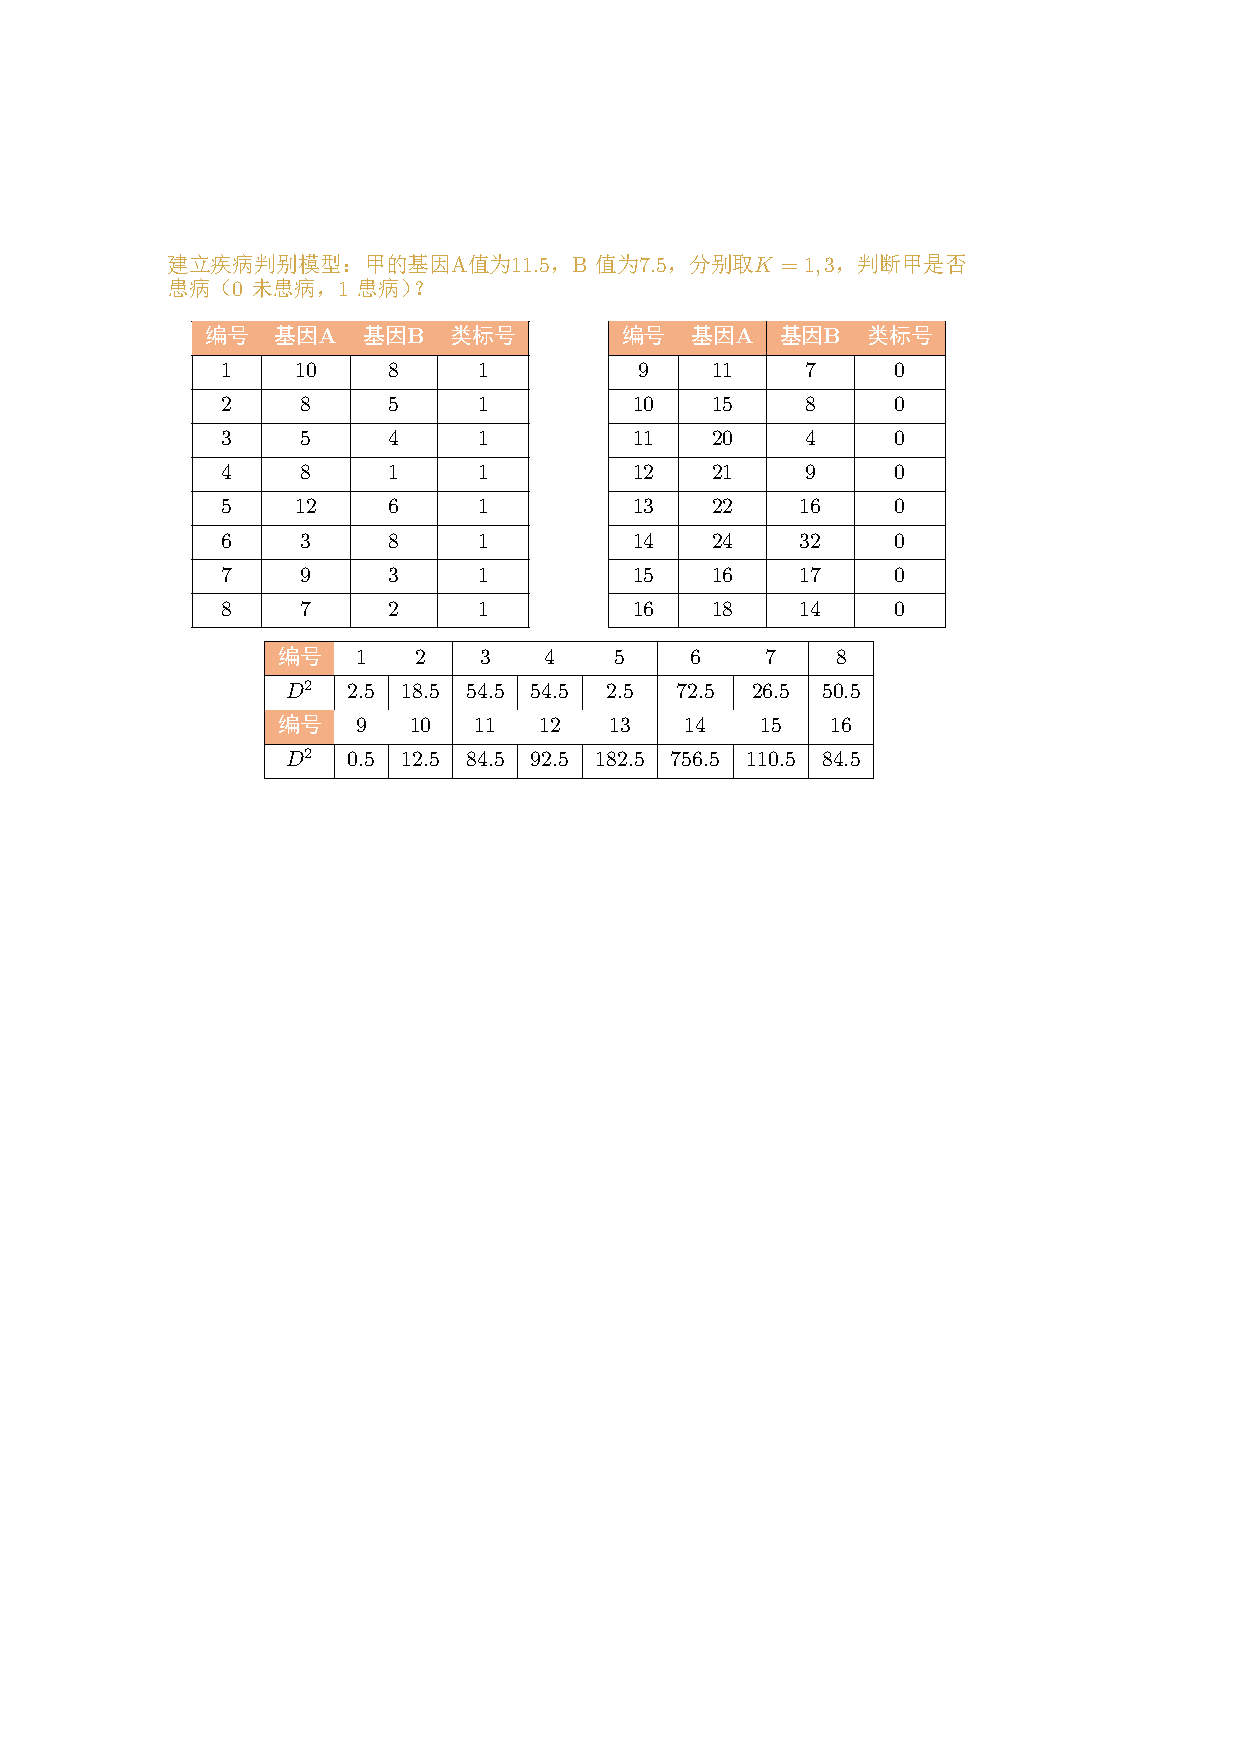
\includegraphics[scale = 0.95]{image/K近邻.pdf}
\end{figure}
\begin{itemize}
    \item $K = 1$,未患病。
    \item $K = 3$,患病。
\end{itemize}
\textcolor{main1}{K近邻法的优点}
\begin{itemize}
    \item 简单,易于理解,易于实现,无需参数估计,无需训练;
    \item 对异常值不敏感,个别噪音数据对结果的影响不是很大;
    \item 适合对稀有事件进行分类;
    \item 适合于多分类问题,K 近邻要比支持向量机表现要好。
\end{itemize}
\textcolor{main1}{K近邻法的缺点}
\begin{itemize}
    \item 对测试样本分类时的计算量大,内存开销大,需要计算新样本到全体已知样本的距离,才能求得它的K 个最近邻点;
    \item 当样本不平衡时,可能导致新样本的K 个邻居中大容量类的样本占多数,出现系统分类偏差;
    \item K近邻是一种消极学习方法、懒惰算法。
\end{itemize}

\textcolor{main1}{决策树}

\begin{note}
    决策树学习的关键是:选择最优划分属性
    \begin{itemize}
        \item 什么样的划分属性是最优的?
        
        希望决策树的分支结点所包含的样本尽可能属于同一类别,即结点的“纯度”越来越高,可以高效地从根结点到达叶结点,得到决策结果。
        \item 三种度量结点“纯度”的指标
        \begin{itemize}
            \item 信息增益:ID3
            \item 增益率:C4.5
            \item 基尼指数:CART
        \end{itemize}
    \end{itemize}
\end{note}
\begin{note}
    决策树的优缺点:
    \begin{itemize}
        \item 优点
        \begin{itemize}
            \item 计算复杂度不高;
            \item 可解释性强;
            \item 能处理具有许多属性的数据集;
            \item 在相对短的时间内能够对大数据集做出可行且效果良好的分类结果。
        \end{itemize} 
        \item 缺点
        \begin{itemize}
            \item 可能存在过拟合问题
        \end{itemize} 
    \end{itemize}
\end{note}

\begin{note}
    剪枝是解决决策树过拟合的一种方法:——通过主动去掉一些分支来降低过拟合的风险

    \begin{itemize}
        \item 预剪枝:
        
        在决策树生成过程中,对每个结点在划分前先进行估计,若当前结点的划分不能带来决策树泛化性能提升,则停止划分并将当前结点标记为叶结点。
        \item 后剪枝:
        
        先从训练集生成一棵完整的决策树,然后自底向上地对非叶结点进行考察,若将该结点对应的子树替换为叶结点能带来决策树泛化性能提升,则将该子树替换为叶结点。
    \end{itemize}
\end{note}

\begin{note}
    在医疗诊断等应用场景中,\textcolor{main1}{灵敏度、特异度、阳性预测值、阴性预测值}等比单纯的错误率 准确率更重要。
    \begin{figure}[htbp]
        \centering
        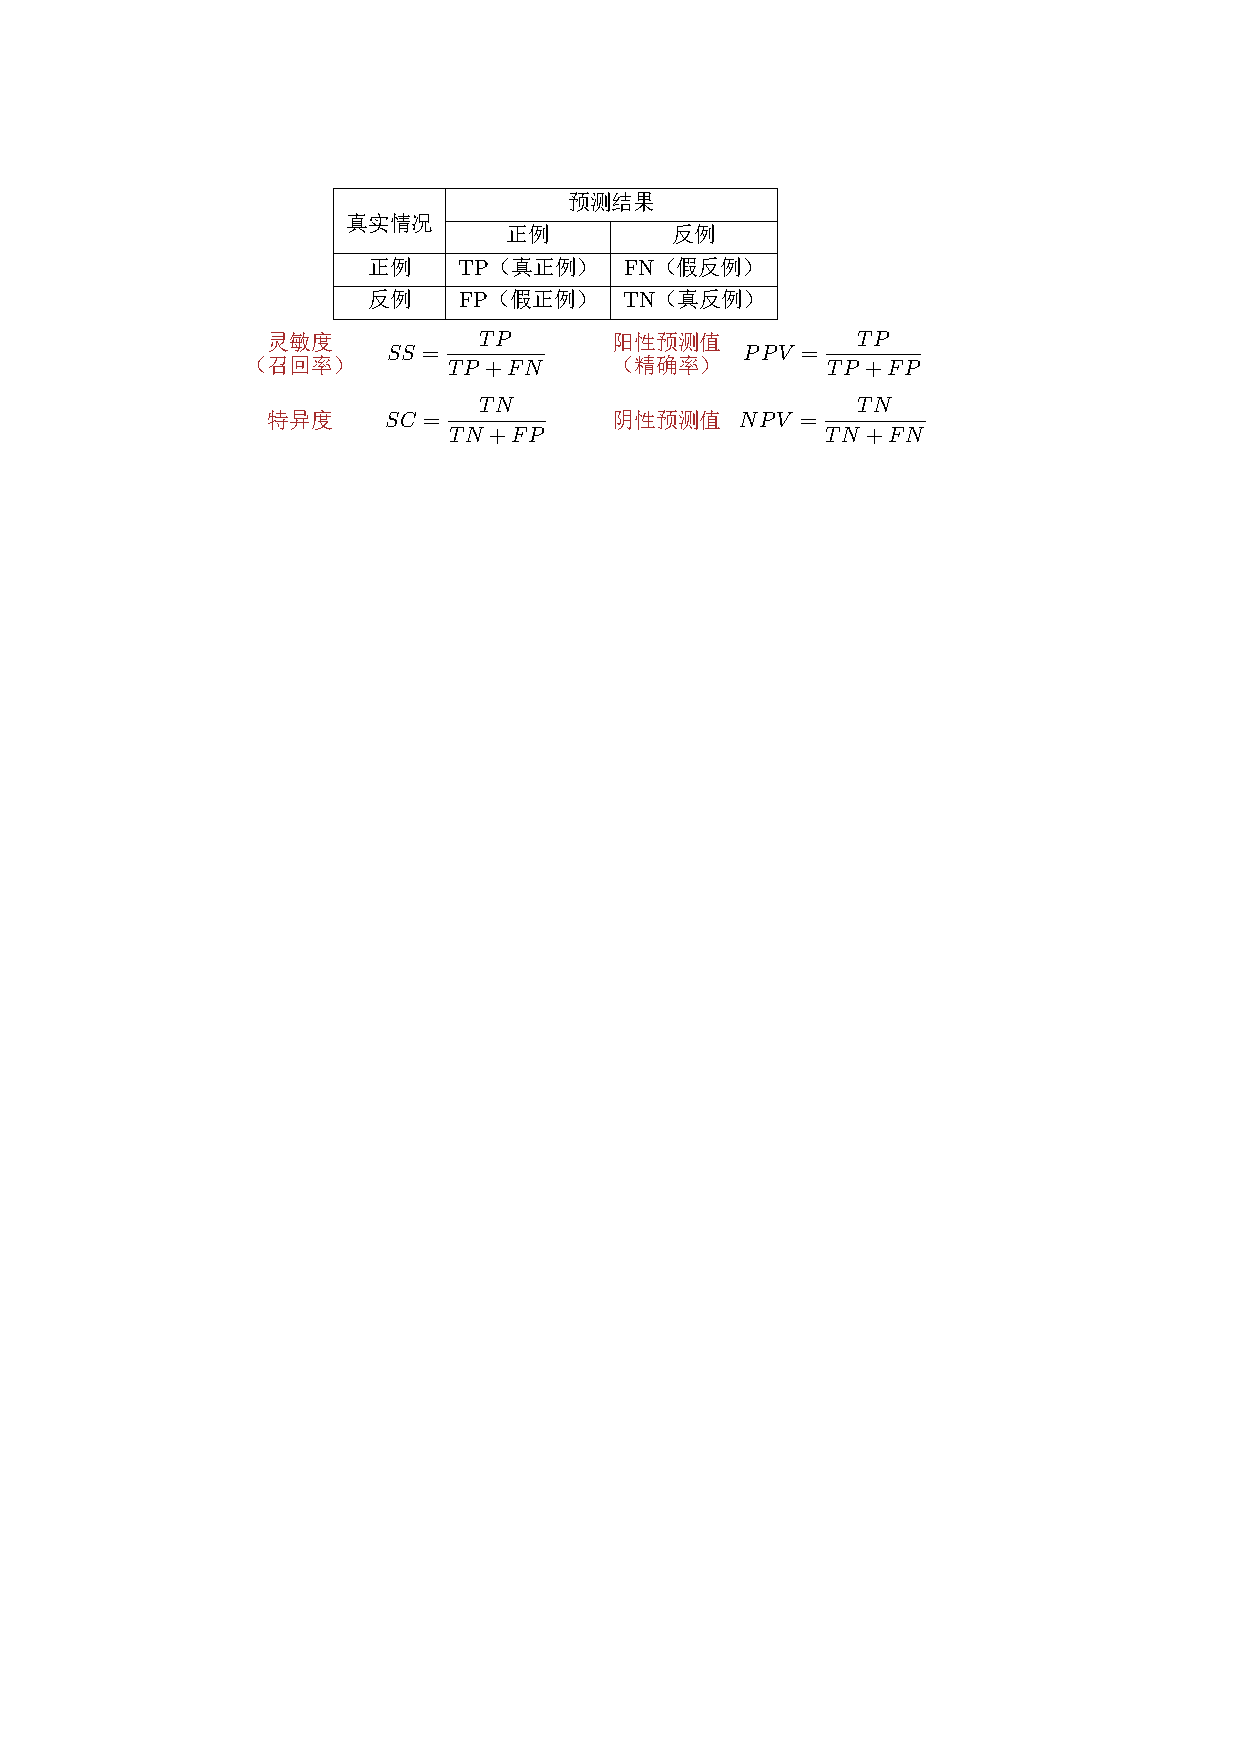
\includegraphics{image/决策树.pdf}
    \end{figure}
\end{note}
\begin{example}
    已知某核酸检测分类器对COVID 19 阳性和阴性样本预测的混淆矩阵如下表所示,该分类方法的灵敏度为\textcolor{main1}{[$\dfrac{3}{3+7} = 30\%$]} 、特异度为\textcolor{main1}{[$\dfrac{9}{1+9} = 90\%$]} 、准确率为\textcolor{main1}{[$\dfrac{3+9}{20} = 30\%$]}。
    \begin{figure}[htbp]
        \centering
        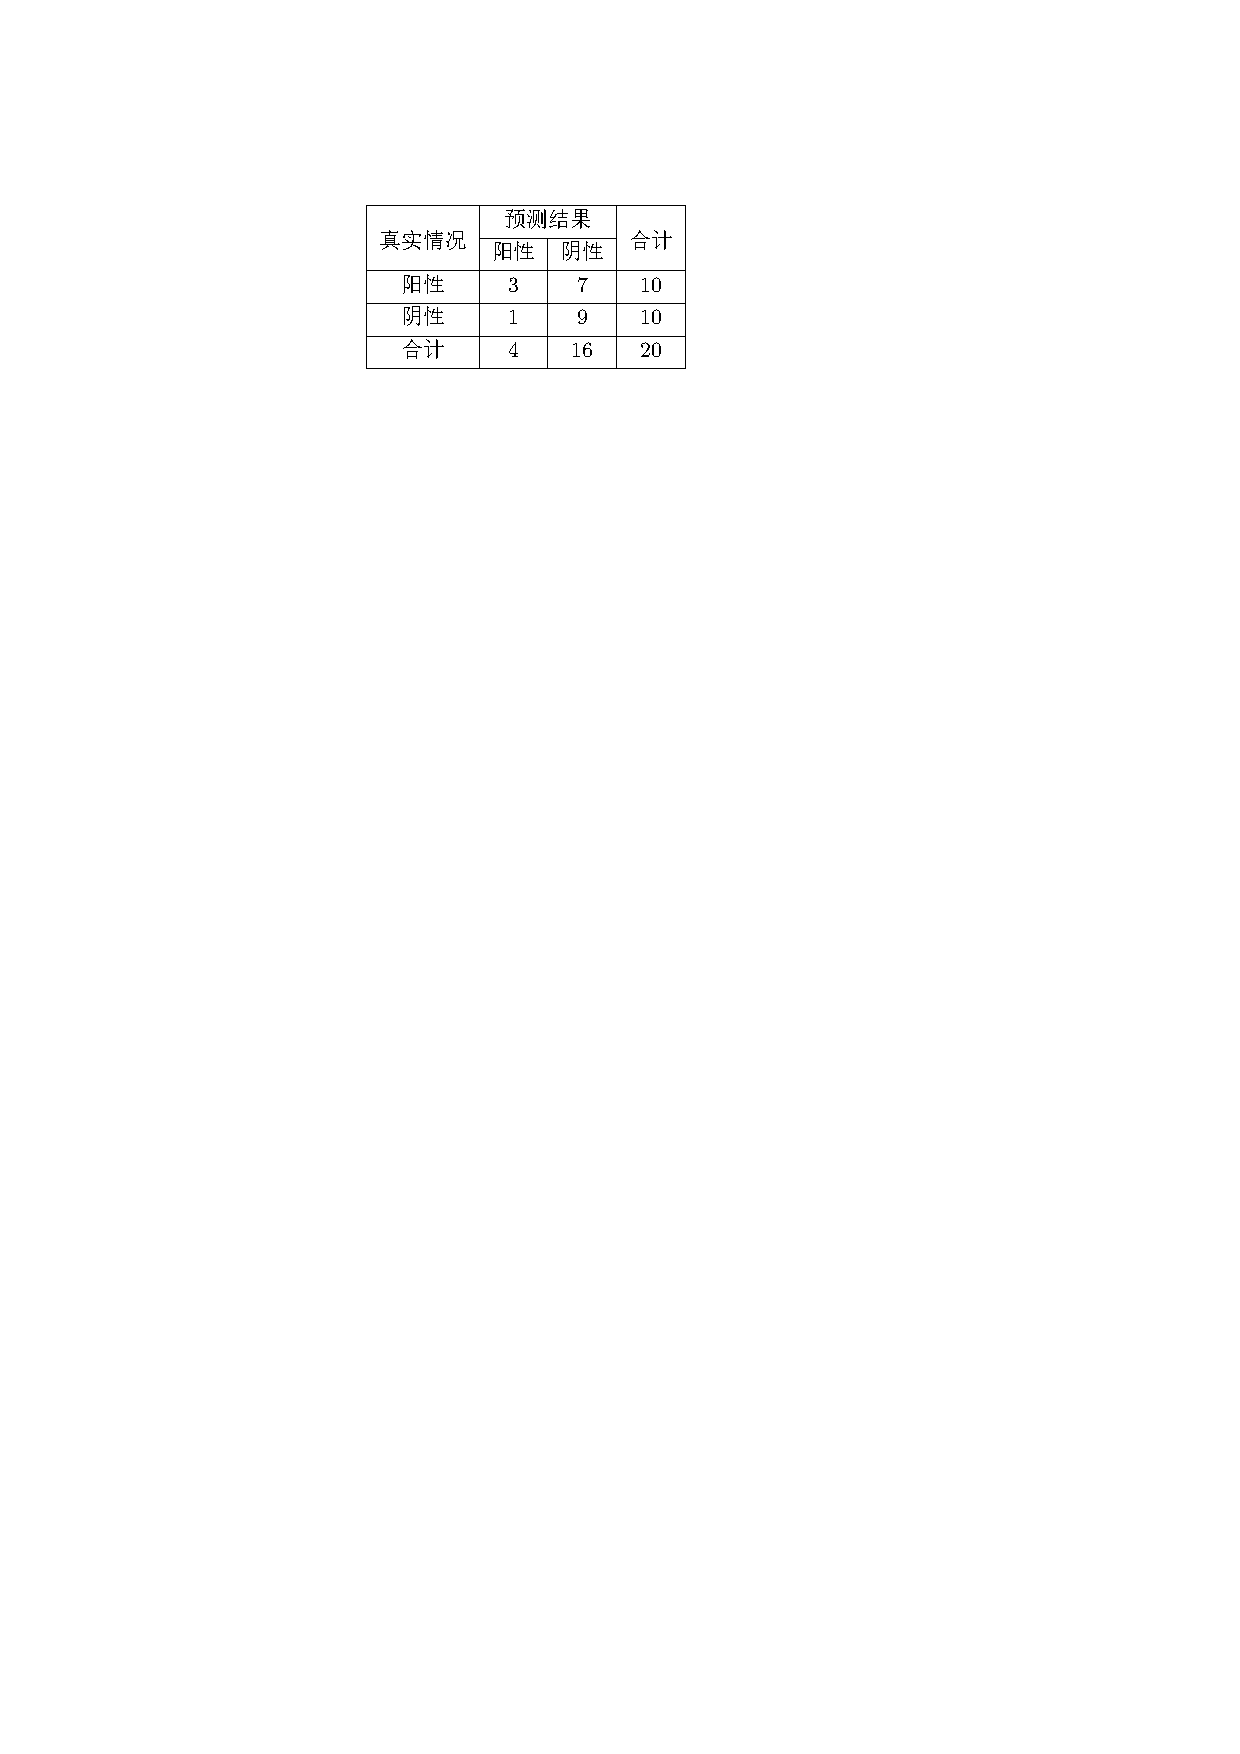
\includegraphics{image/混淆矩阵例题.pdf}
    \end{figure}
\end{example}
\subsection{无监督学习基本方法}
\textcolor{main1}{无监督学习(聚类)的一般过程}
\begin{definition}[无监督学习]
    根据数据的相似性将数据分为多类的过程。
\end{definition}
\textcolor{main1}{目标}:将数据集中的样本按照相似性划分为若干个通常不相交的子集“簇”。
\begin{figure}[htbp]
    \centering
    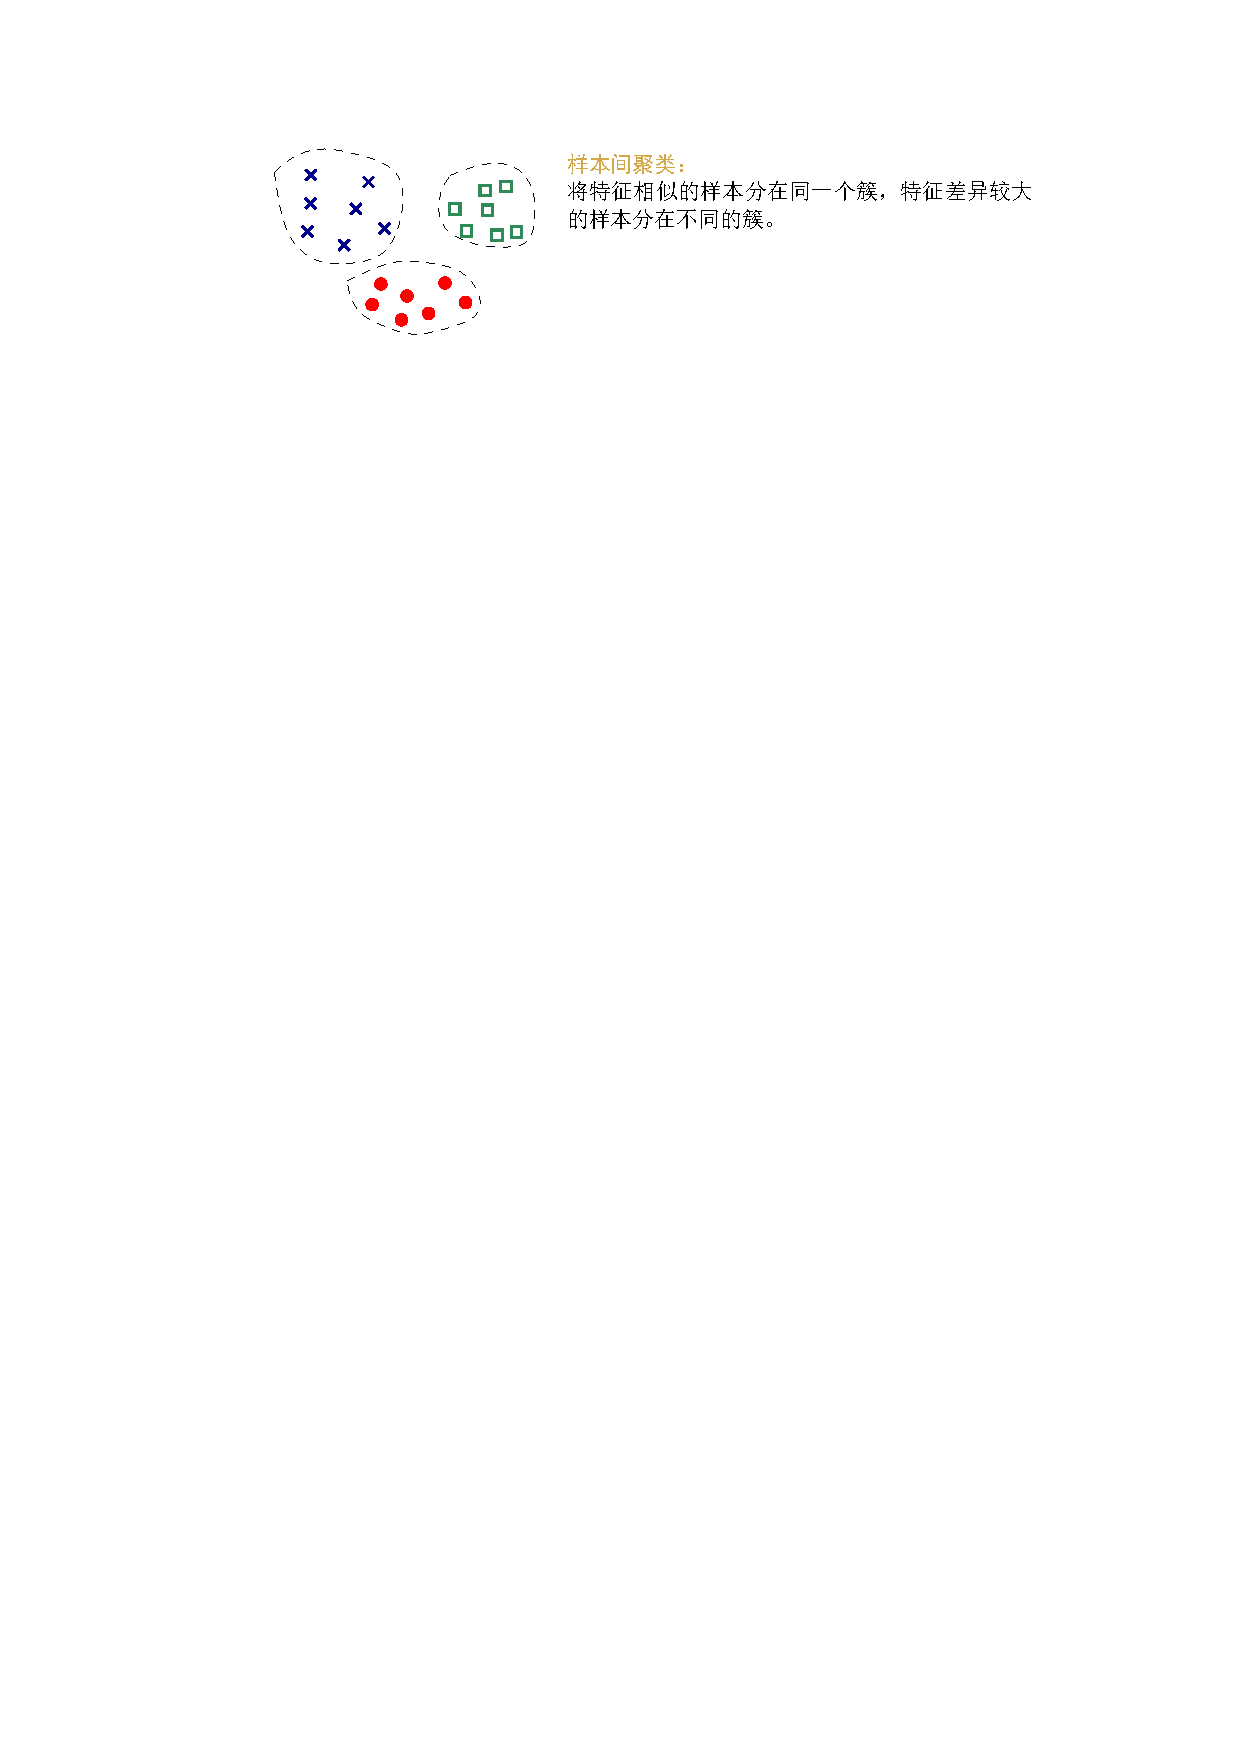
\includegraphics{image/聚类目标.pdf}
\end{figure}
\subsubsection{相似性的度量}
\textcolor{main1}{闵可夫斯基距离}

\begin{definition}[闵可夫斯基距离]
    设$\boldsymbol{x}_{i} = \left( x_{i1},\cdots,_{ip} \right)$和$\boldsymbol{x}_{j} = \left( x_{j1},\cdots,_{jp} \right)$是$i$和$j$哥样本的特征向量,则二者之间的距离为
    \[
        d_{ij} = \left( \sum\limits_{k = 1}^{p}|x_{ik}-x_{jk}|^{g} \right)^{1/g}
    \]
    \begin{itemize}
        \item 当$g = 1$时(绝对值距离),$d_{ij} = \sum\limits_{k = 1}^{p}|x_{ik}-x_{jk}|$
        \item 当$g = 2$时(欧式距离),$d_{ij} = \sqrt{\sum\limits_{k = 1}^{p}\left( x_{ik}-x_{jk} \right)^2}$
    \end{itemize}
\end{definition}
\begin{note}
    闵式距离的缺陷
    \begin{itemize}
        \item 容易受变量的量纲影响
        \item 没有考虑变量间的相关性
    \end{itemize}
\end{note}
\begin{note}
    两种改进措施
    \begin{itemize}
        \item $\text{变量标准化处理}\left\{ \begin{array}{ll}
            \text{极差标准化} & y_i = \dfrac{x_{i}-\min x}{\max x-\min x} \\
            \text{Z-score标准化} & z_i = \dfrac{x_i-\operatorname{mean}(x)}{\sigma}
        \end{array} \right.$
        \item 马氏距离 $ D_{M}(x) = \sqrt{\left( \boldsymbol{x}-\boldsymbol{\mu} \right)^{\mathrm{T}}\boldsymbol{S}^{-1}\left( \boldsymbol{x}-\boldsymbol{\mu} \right)}$
    \end{itemize}
\end{note}
\textcolor{main1}{方向余弦度量相似度}
\begin{definition}[方向余弦]
    $n$维向量$x$和$y$的夹角记作$\theta$,根据余弦定理,其余弦值为
    \[
        \cos (\theta) = \dfrac{\boldsymbol{x}^{\mathrm{T}}\boldsymbol{y}}{|\boldsymbol{x}||\boldsymbol{y}|} = \dfrac{\sum\limits_{k = 1}^{p}x_{ik}x_{jk}}{\sqrt{\sum\limits_{k = 1}^{p}x_{ik}^2 \sum\limits_{k = 1}^{p}x_{jk}^2}}
    \]
\end{definition}

\textcolor{main1}{相关系数}
\begin{definition}[相关系数]
    设$\boldsymbol{x}_{i} = \left( x_{i1},\cdots,_{ip} \right)$和$\boldsymbol{x}_{j} = \left( x_{j1},\cdots,_{jp} \right)$是$i$和$j$哥样本的特征向量,则二者之间的相关系数为
    \[
        r_{ij} = \dfrac{\sum\limits_{k = 1}^{p}\left( x_{ik}-\bar{x_{i}} \right)\left( x_{jk}-\bar{x_{j}} \right)}{\sqrt{\left[\sum\limits_{k = 1}^{p} \left( x_{ik}-\bar{x_{i}} \right)^2 \right]\left[\sum\limits_{k = 1}^{p} \left( x_{jk}-\bar{x_{j}} \right)^2 \right]}}
    \]
\end{definition}
\begin{note}
    相关系数和方向余弦关系
    \begin{figure}[htbp]
        \centering
        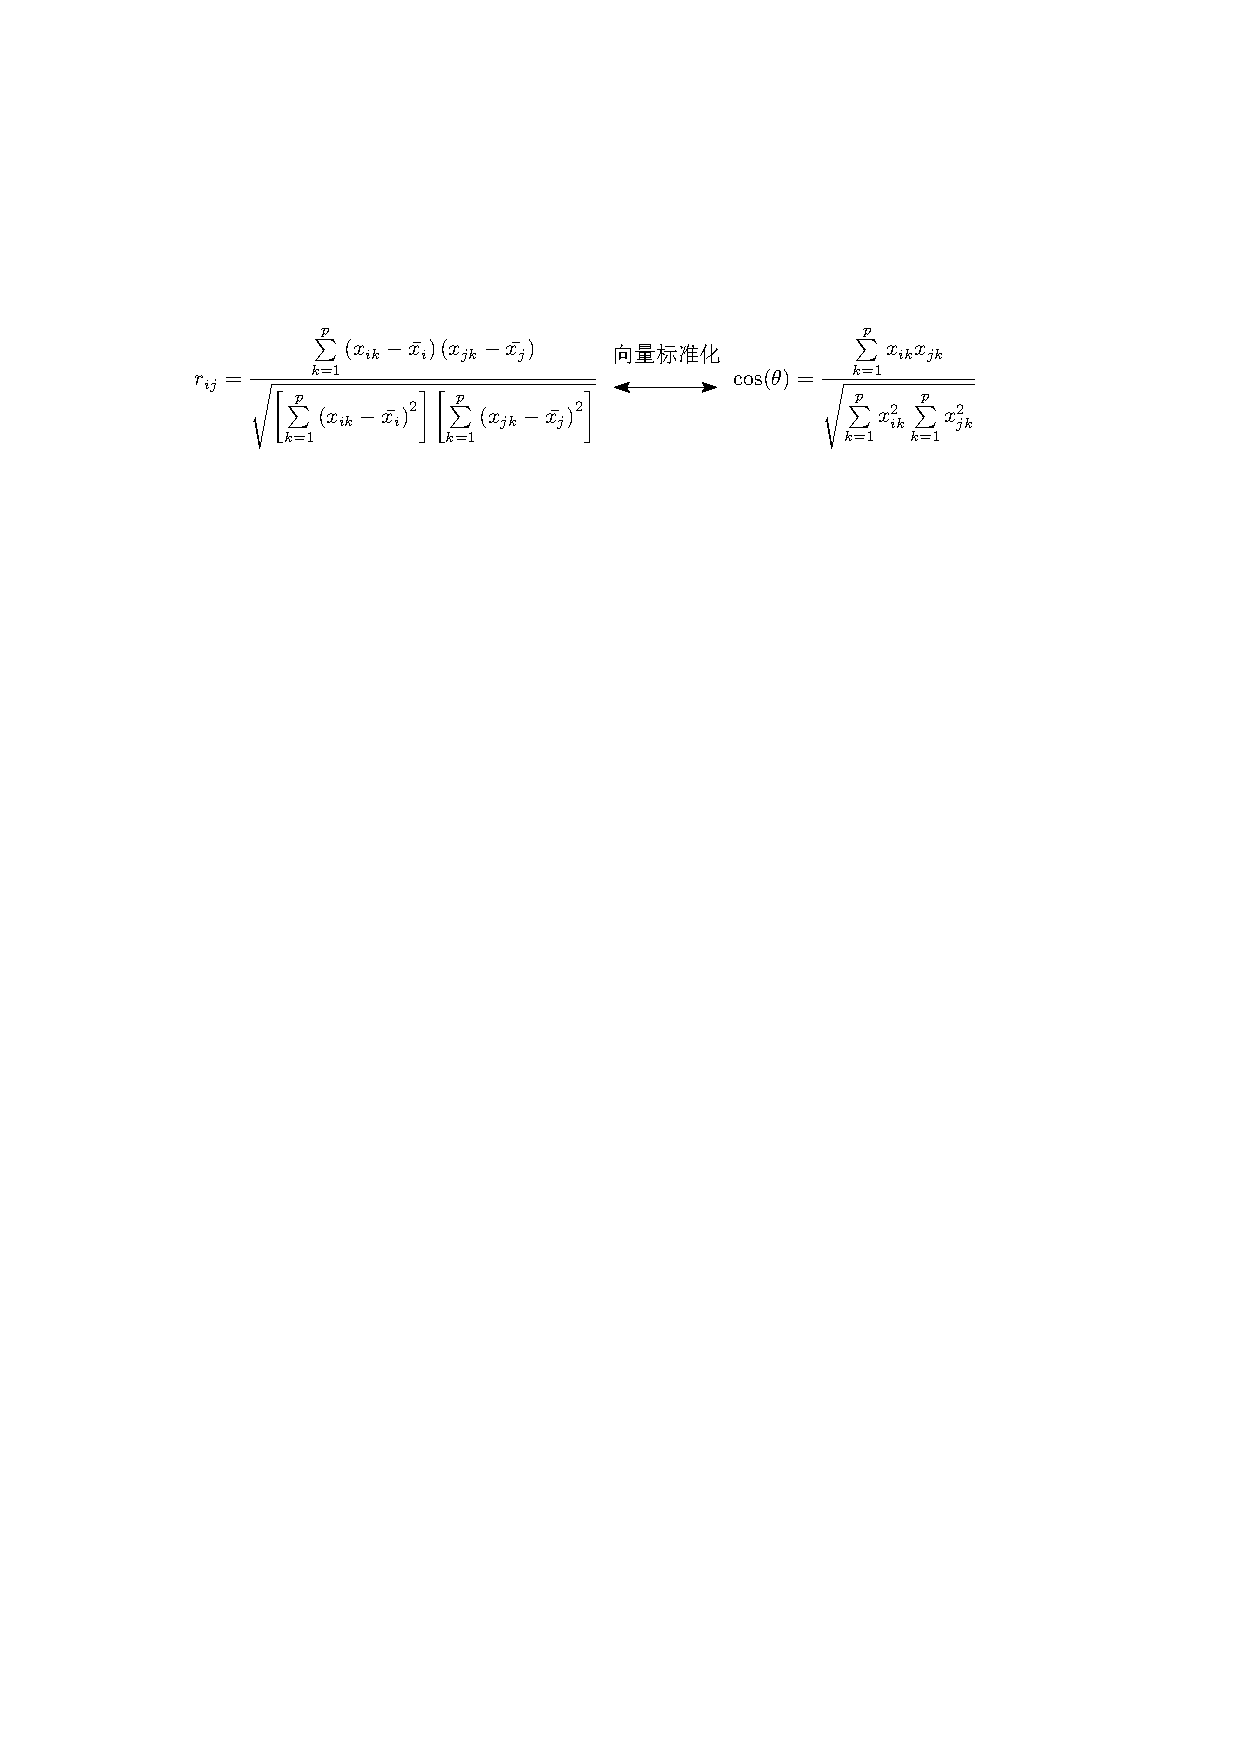
\includegraphics{image/余弦和相关系数关系.pdf}
    \end{figure}
\end{note}
\begin{note}
    常用聚类方法:
    \begin{itemize}
        \item 划分法:\textcolor{main1}{需要输入类别数},适用于\textcolor{main2}{样本数较多}的情况
        \item 层次法:\textcolor{main1}{不需要输入类别数},适用于\textcolor{main2}{样本数较少}的情况
    \end{itemize}
\end{note}
\subsubsection{划分法}
\begin{definition}[划分法]
    给定一个有$N $个样本的数据集,划分法将构造$K $个分组,每一个分组就代表一个聚类,$K<N$ 。而且这$K $个聚类满足两个条件:
    \begin{itemize}
        \item 每一个聚类至少包含一个样本;
        \item 每一个样本属于且仅属于一个聚类。
    \end{itemize}

    \textcolor{main1}{标准:}同一聚类中的样本相似性高,不同聚类中的样本相似性低

    \textcolor{main1}{典型算法:}K 均值聚类算法、K MEDOIDS 算法、CLARANS 算法
\end{definition}

\textcolor{main1}{K均值聚类}
\begin{note}
    基本思想
    
    将每一个样本分配到最近中心(样本均值)所属的簇

    \textcolor{main1}{目标函数:}$C^{*} = \arg\min\limits_{C}\sum\limits_{l = 1}^{K}\sum\limits_{C(i) = l}\|\boldsymbol{x}_i-\bar{\boldsymbol{x}_l}\|^2$

    \textcolor{main1}{优化方法:}采用贪心策略,通过迭代优化来近似求解,不能保证收敛到全局最优

    算法主要包括以下步骤:
    \begin{enumerate}
        \item 指定聚类数,确定初始簇的中心
        
        用户指定或系统指定。
        \item 根据距离最近原则进行分类
        
        计算每个样本到各簇中心点的距离, 并按距离最近原则对所有样本进行分类,计算新的聚类中心。
        \item 迭代,直至收敛
    \end{enumerate}
\end{note}
\begin{example}
    对A 、B 、C 、D 样本分别测量特征$X_1$ 和$X_2$,得到如下结果。
    \begin{figure}[htbp]
        \centering
        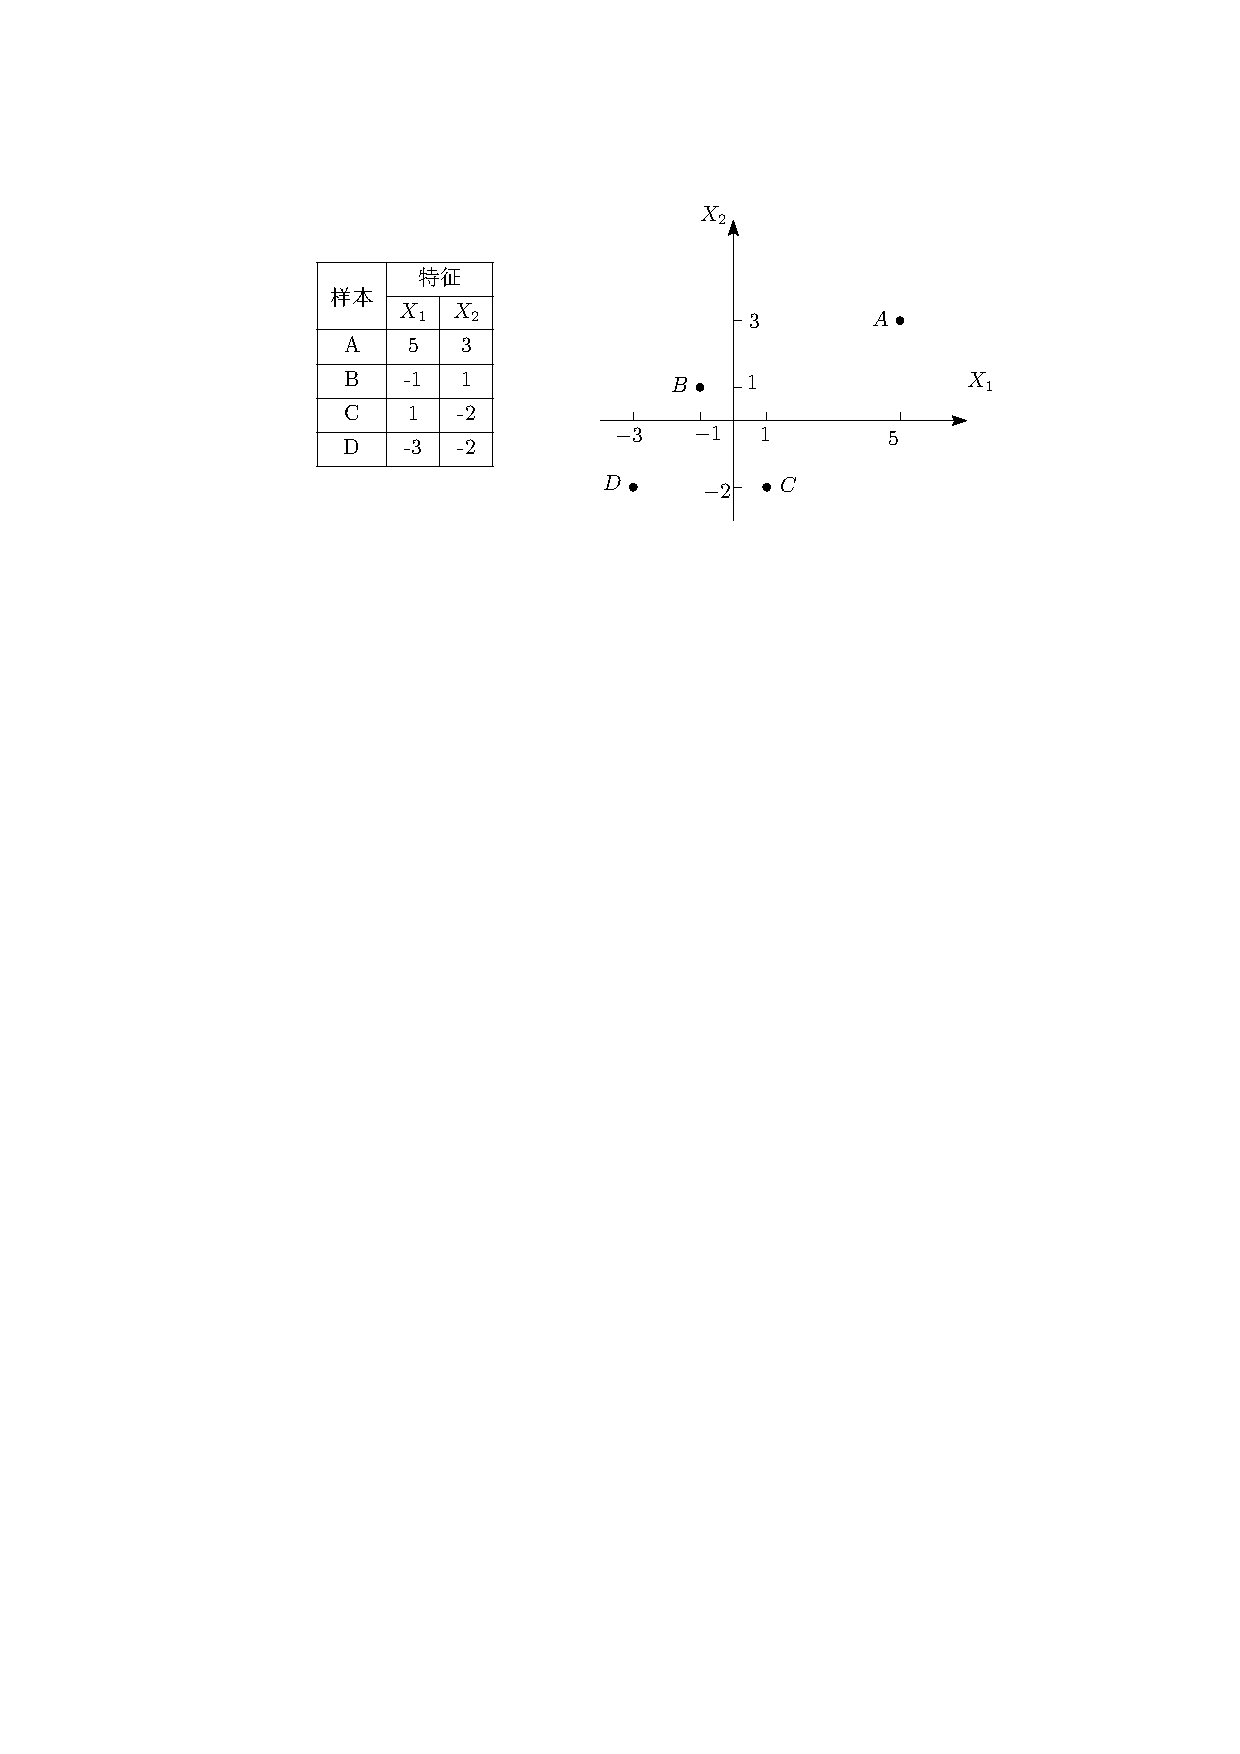
\includegraphics{image/K均值.pdf}
    \end{figure}
    试用K 均值方法将这四个样本聚成两簇。
    \begin{enumerate}
        \item 按要求取$K = 2$,将样本随意分成两簇(A,B)和(C,D),计算两个聚类的中心坐标。计算样本到各簇中心的欧氏距离,将样本分配给最近的一簇。对于样本有变动的簇,重新计算它们的中心坐标。
        % Table generated by Excel2LaTeX from sheet 'K均值'
        \begin{table}[htbp]
            \centering
            \begin{tabular}{|c|c|c|c|c|c|c|}
            \hline
            \multirow{2}[4]{*}{聚类} & \multicolumn{2}{c|}{中心坐标} & \multicolumn{4}{c|}{$D^2(i,C_l)$} \bigstrut\\
        \cline{2-7}        & $X_1$ & $X_2$ & A   & B   & C   & D \bigstrut\\
            \hline
            $(A,B)$ & 2   & 2   & 10  & 10  & 17  & 41 \bigstrut\\
            \hline
            $(C,D)$ & -1  & -2  & 61  & 9   & 4   & 4 \bigstrut\\
            \hline
            \end{tabular}%
        \end{table}%

        B被分配到$(C,D)$
        \item 再次检查每个样本,以决定是否需要重新分簇。计算样本到各中心的距离。
        % Table generated by Excel2LaTeX from sheet 'K均值'
        \begin{table}[htbp]
            \centering
            \begin{tabular}{|c|c|c|c|c|c|c|}
            \hline
            \multirow{2}[4]{*}{聚类} & \multicolumn{2}{c|}{中心坐标} & \multicolumn{4}{c|}{$D^2(i,C_l)$} \bigstrut\\
        \cline{2-7}        & $X_1$ & $X_2$ & A   & B   & C   & D \bigstrut\\
            \hline
            $(A)$ & 5   & 3   & 0   & 40  & 41  & 89 \bigstrut\\
            \hline
            $(B,C,D)$ & -1  & -1  & 52  & 4   & 5   & 5 \bigstrut\\
            \hline
            \end{tabular}%
        \end{table}%
        
        由于每个样本都已经分配到距离中心最近的簇,因此聚类过程到此结束。最终得到$K=2 $的聚类结果是$A $独自成一簇,$B,\,C,\,D $聚成一簇。
    \end{enumerate}
\end{example}
\begin{example}
    请判断以下说法是否正确:当距离度量和聚类数目选定后,$K $均值聚类的结果是唯一的。
    \begin{enumerate}[A]
        \item 正确
        \item \textcolor{main1}{错误}
    \end{enumerate}
\end{example}
\begin{note}
    $K $均值聚类:优缺点
    \begin{itemize}
        \item 优点
        \begin{itemize}
            \item 简单快速,可以用于多种数据类型
            \item 有效,可处理大数据集
        \end{itemize}
        \item 缺点
        \begin{itemize}
            \item 结果受初始聚类中心影响较大
            \item 不适合处理非球形簇、不同尺度和不同密度的簇
            \item 结果受聚类数影响较大
            \item 对噪声和孤立点数据敏感
        \end{itemize}
    \end{itemize}
\end{note}
\begin{note}
    均值聚类的改进
    \begin{itemize}
        \item 初始聚类中心的选择
        \begin{itemize}
            \item 选择彼此距离尽可能远的$K $个点
            \item 选择密度最大的$K $个点
        \end{itemize}
        \item 聚类数的选择
        \begin{itemize}
            \item 观察法
            \item 肘部法
            \begin{itemize}
                \item 随着聚类数$K $增大,样本划分更加精细,每个簇的聚合程度逐渐提高,误差平方和变小;
                \item 当$K $小于真实聚类数时, $K $增大会大幅增加每个簇的聚合程度,误差平方和的下降幅度很大;
                \item 当$K $到达真实聚类数时,误差平方和的下降幅度骤减,然后随着$K $值的继续增大而趋于平缓;
                \item 误差平方和与$K $的关系图是一个手肘的形状,而肘部对应的$K $ 值就是数据的真实聚类数。
            \end{itemize}
        \end{itemize}
        \item 离群点的处理
        \begin{itemize}
            \item 离群点检测和删除
        \end{itemize}
    \end{itemize}
\end{note}
\subsubsection{层次法}
\begin{definition}[层次聚类方法]
    通过计算数据集中样本间的相似性来创建一棵有层次的嵌套聚类树。
\end{definition}

\textcolor{main1}{创建聚类树的策略}
\begin{figure}[htbp]
    \centering
    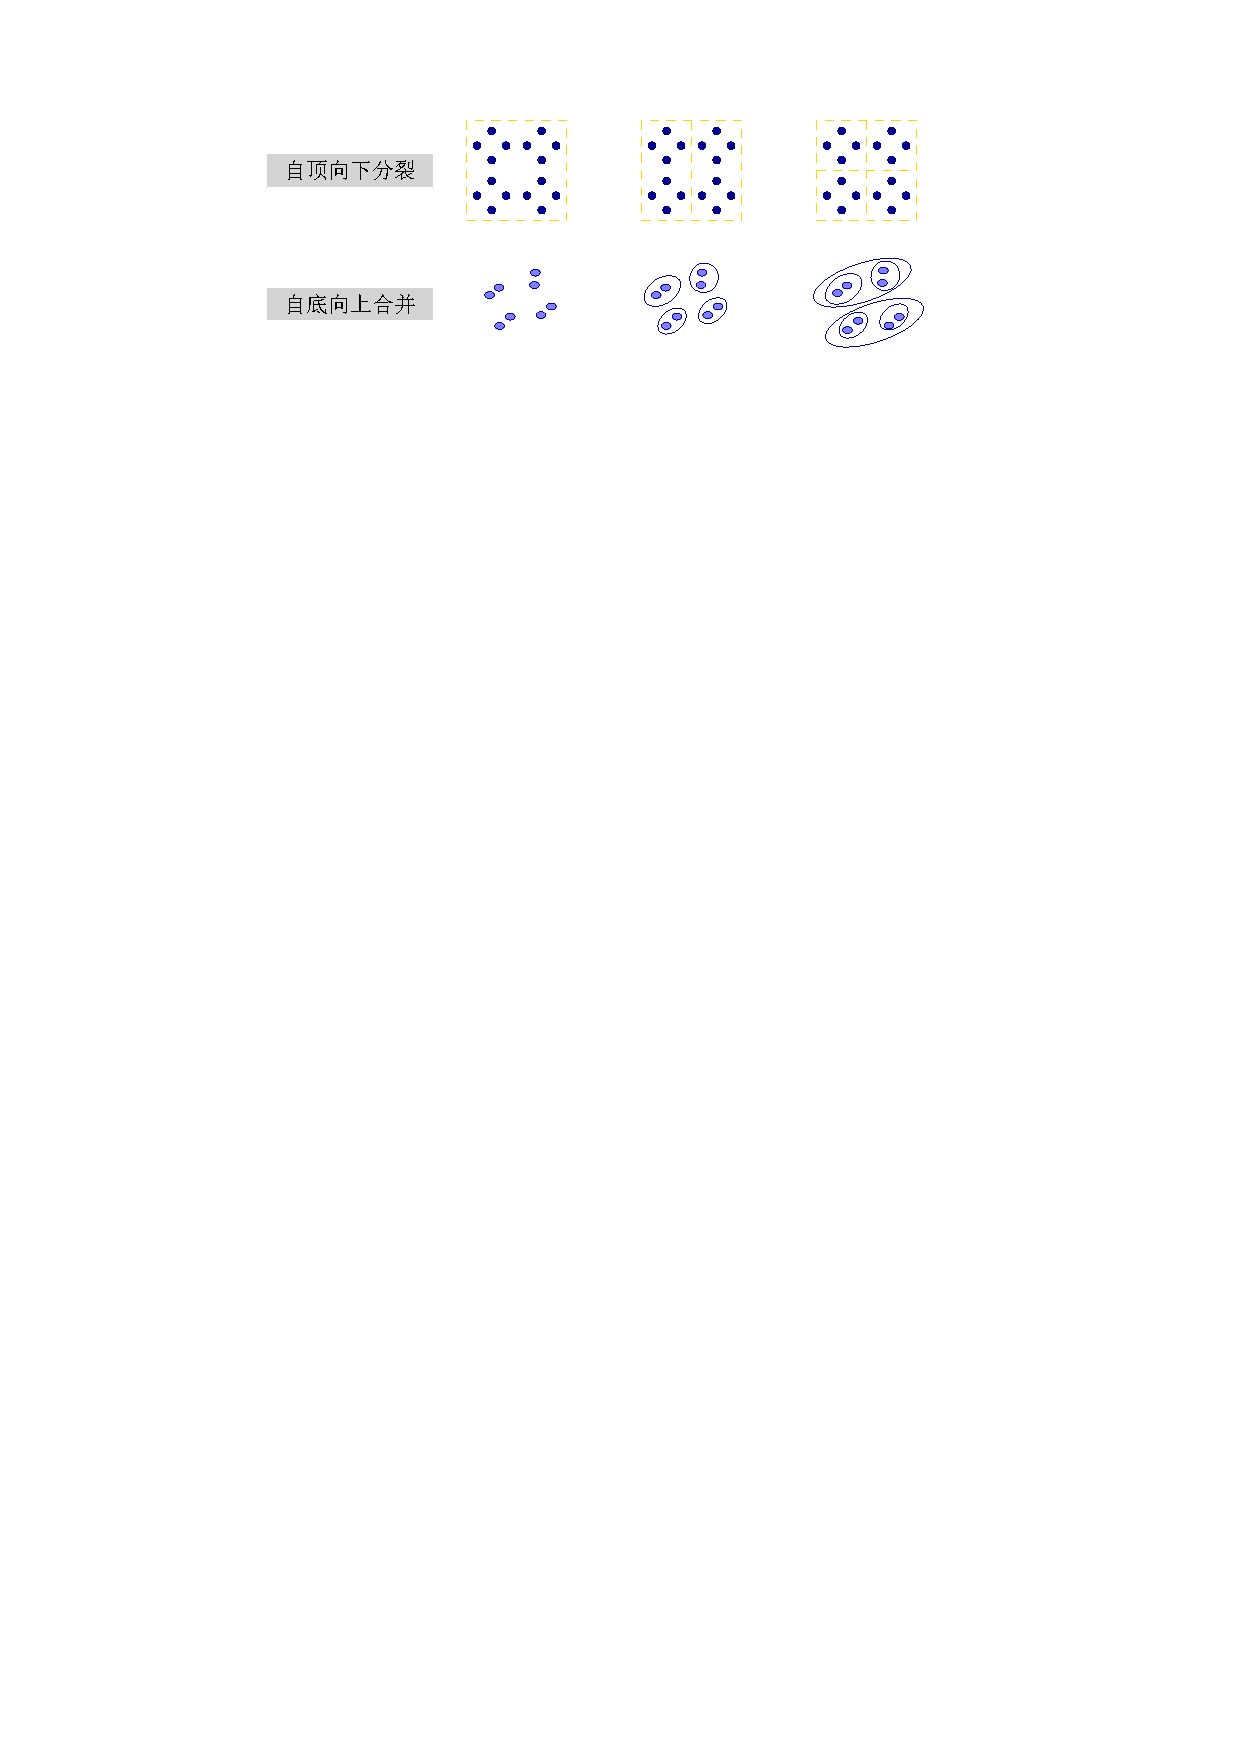
\includegraphics{image/创建聚类树的策略.pdf}
\end{figure}

\textcolor{main1}{自底向上的层次聚类过程}
\begin{figure}[htbp]
    \centering
    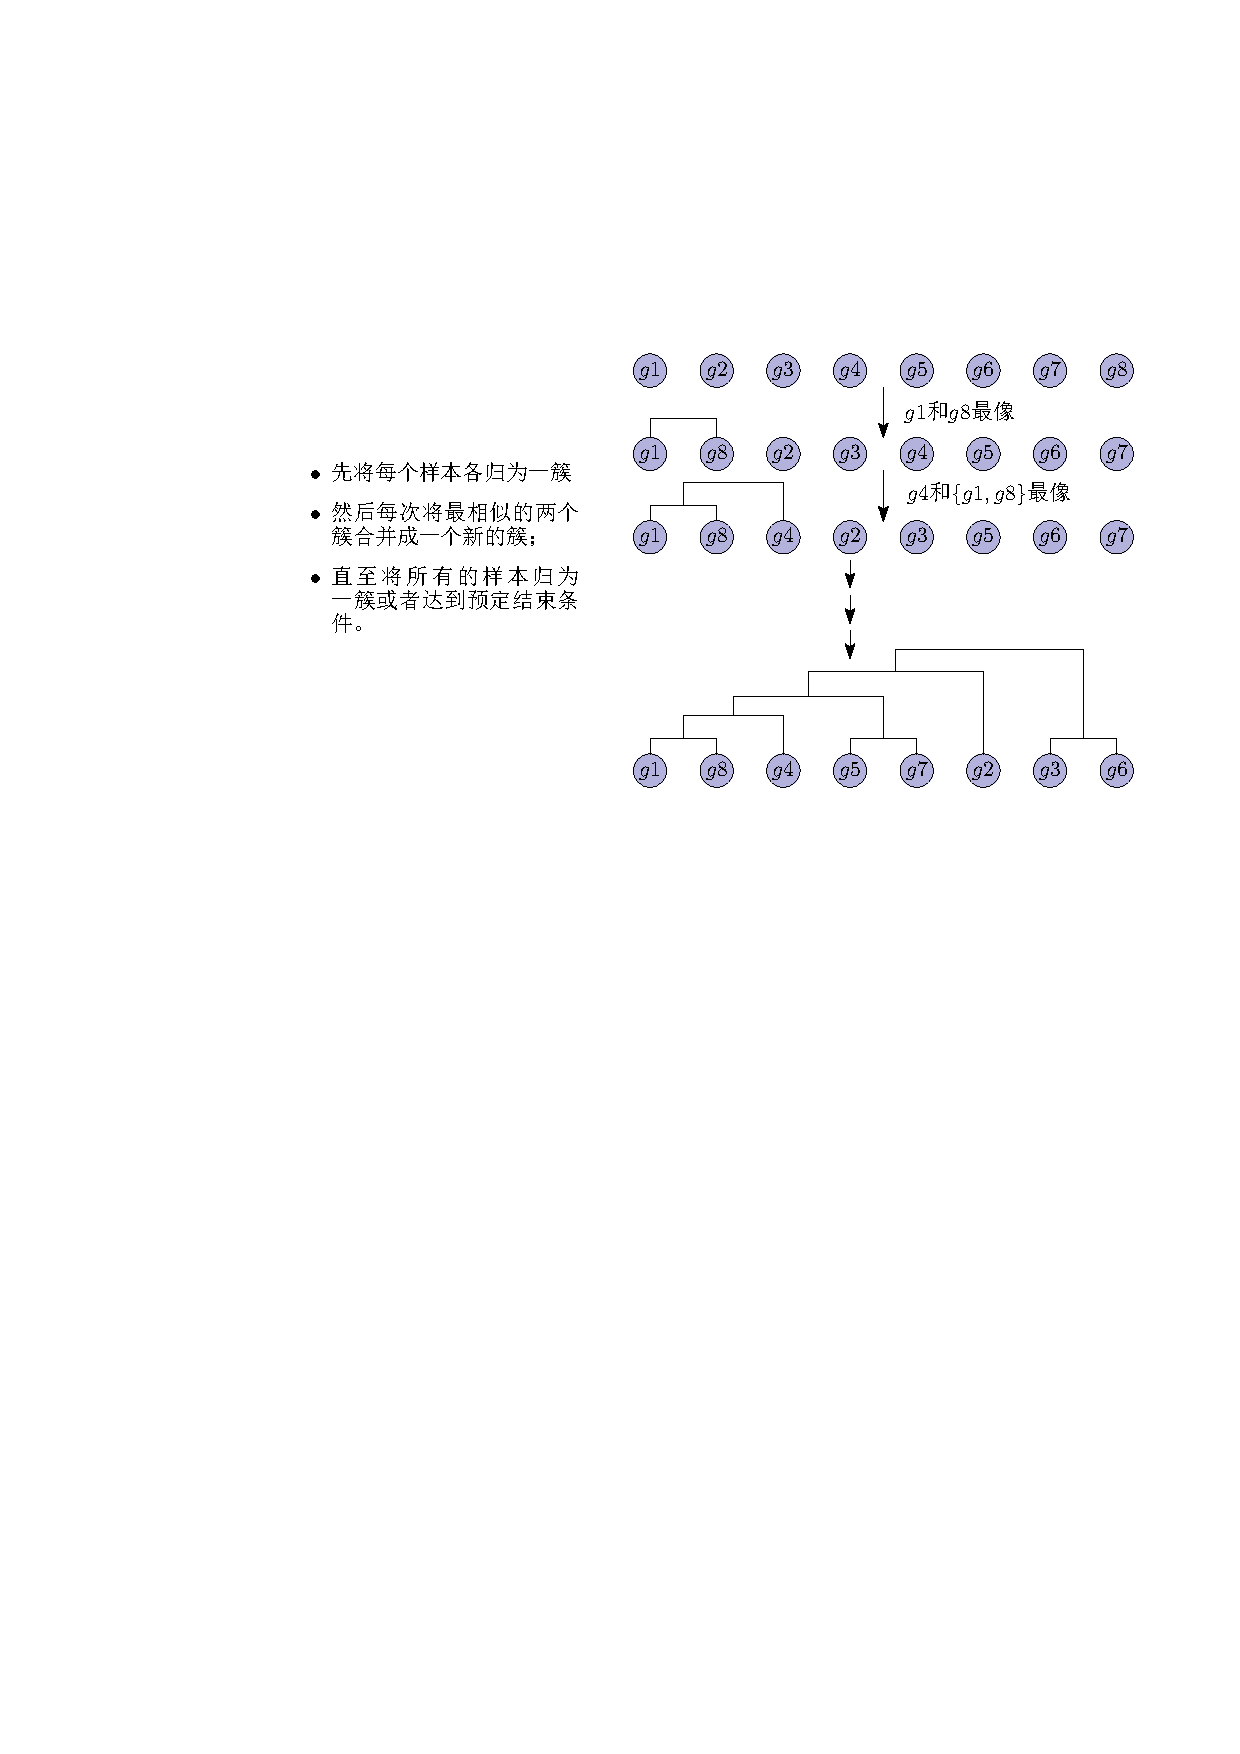
\includegraphics{image/自底向上.pdf}
\end{figure}
\begin{note}
    三个要素:距离度量、合并规则和结束条件
\end{note}
\begin{note}
    思考:

    给定两两样本之间的距离度量函数,对于由两个或者多个样本合并之后得到的新簇,要如何确定它们与其他簇之间的距离呢?
\end{note}
\begin{note}
    \textcolor{main1}{簇间的距离}

    给定据类簇$C_i$和$C_j$
    \begin{itemize}
        \item \textcolor{main1}{最小距离:}$ d_{\min}\left( C_i,C_j \right) = \min\limits_{\boldsymbol{x}\in C_{i},\boldsymbol{z}\in C_{j}} \operatorname{dist}\left( \boldsymbol{x},\boldsymbol{z} \right) $
        \item \textcolor{main1}{最大距离:}$ d_{\max}\left( C_i,C_j \right) = \max\limits_{\boldsymbol{x}\in C_{i},\boldsymbol{z}\in C_{j}} \operatorname{dist}\left( \boldsymbol{x},\boldsymbol{z} \right) $
        \item \textcolor{main1}{平均距离:}$ d_{\operatorname{avg}}\left( C_i,C_j \right) = \dfrac{1}{|C_i||C_j|}\sum\limits_{\boldsymbol{x}\in C_{i}}\sum\limits_{\boldsymbol{z}\in C_{j}} \operatorname{dist}\left( \boldsymbol{x},\boldsymbol{z} \right) $
    \end{itemize}

    \textcolor{main1}{最小距离}由两个簇的\textcolor{main1}{最近样本}决定,\textcolor{main1}{最大距离}由两个簇的\textcolor{main1}{最远样本}决定,而\textcolor{main1}{平均距离}由两个簇的\textcolor{main1}{所有样本}共同决定。
\end{note}

\begin{example}
    层次聚类的结果是不是唯一的?
    \begin{enumerate}[A]
        \item 唯一
        \item \textcolor{main1}{不唯一}
    \end{enumerate}
\end{example}
\begin{example}
    设有6个样本,对每个样本测量一个特征,分别是1、2、5、7、9、10,用基于\textcolor{main1}{最小距离}的层次法将它们分类。
    \begin{figure}[htbp]
        \centering
        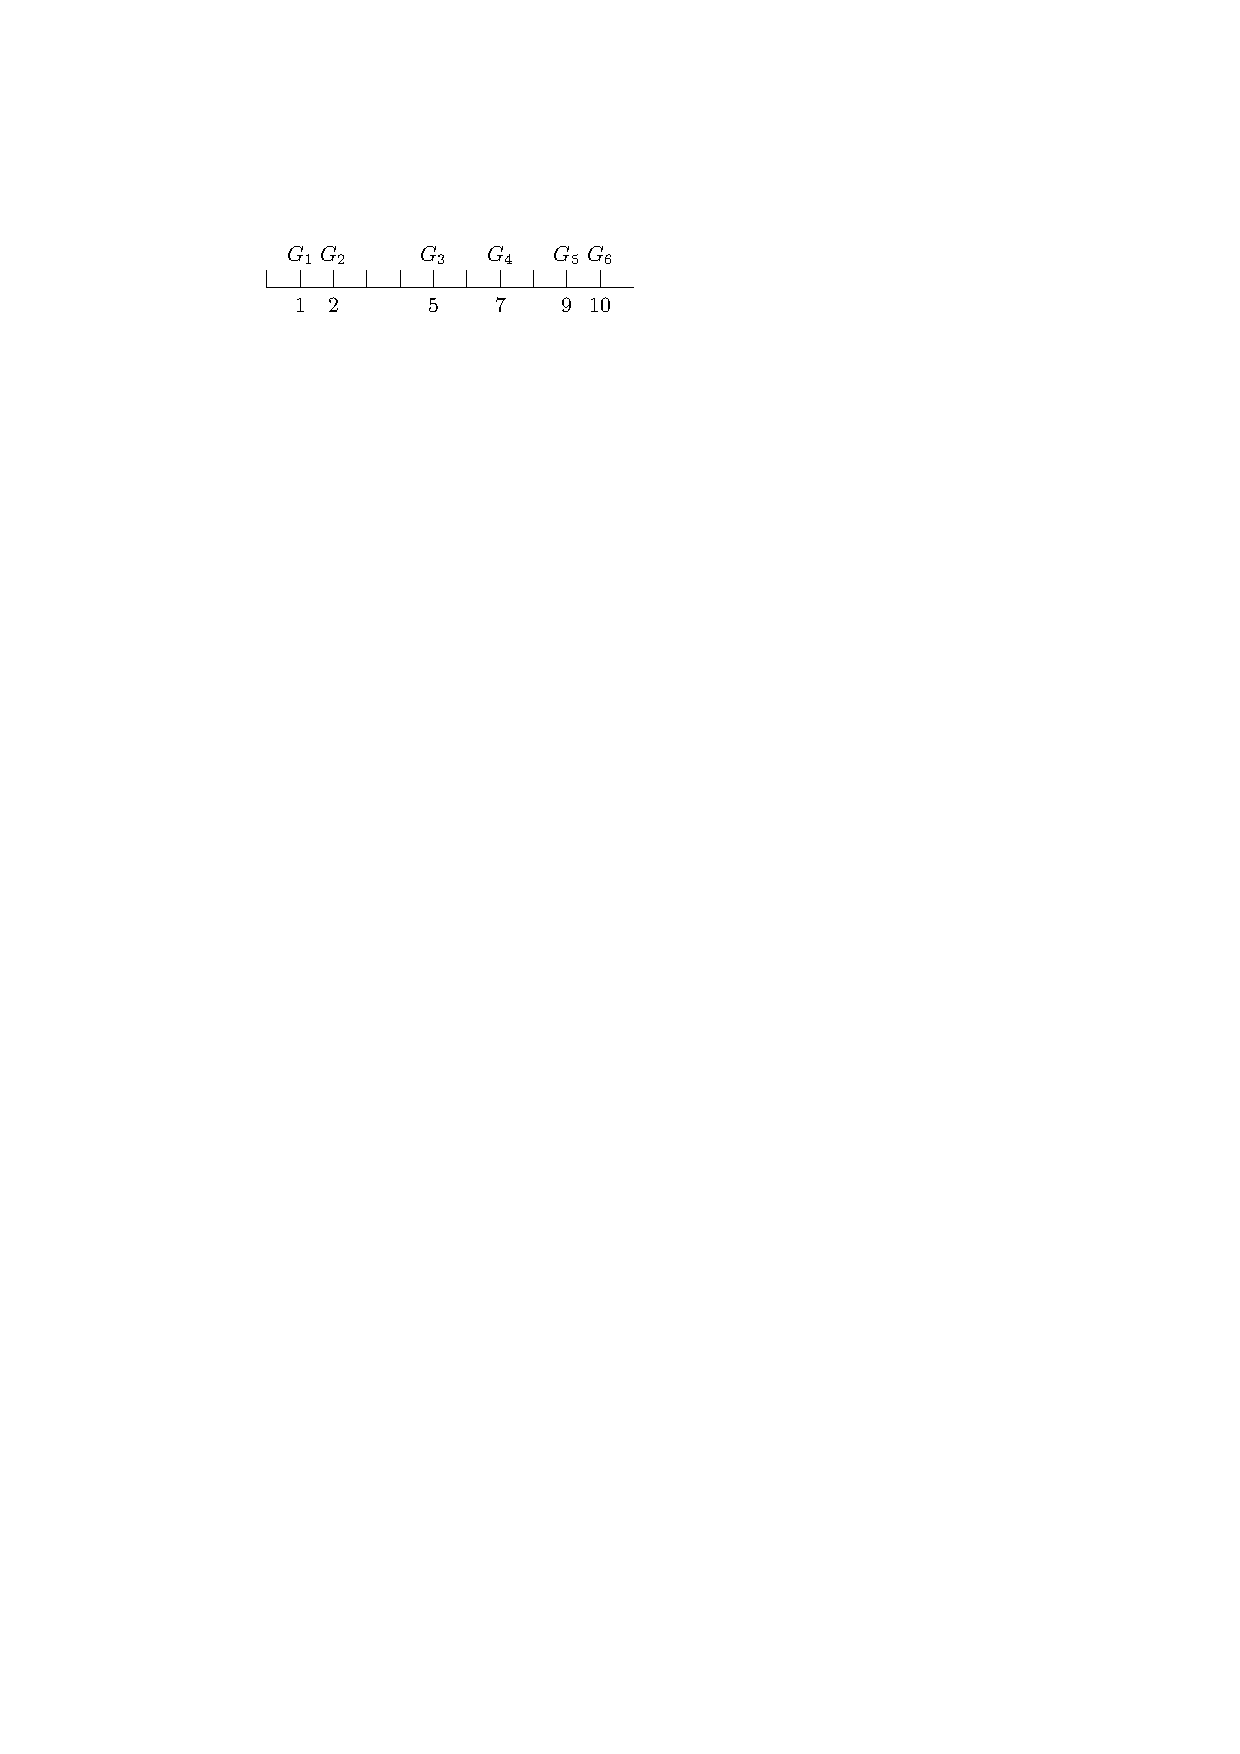
\includegraphics{image/层次聚类举例.pdf}
    \end{figure}
    \begin{enumerate}
        \item 选择绝对距离作为距离度量,形成距离矩阵$D_{(0)}$
        % Table generated by Excel2LaTeX from sheet '层次聚类'
        \begin{table}[htbp]
            \centering
            \begin{tabular}{c|cccccc}
            \hline
                & $G_1$ & $G_2$ & $G_3$ & $G_4$ & $G_5$ & $G_6$ \\
                \hline
            $G_1$ & 0   &     &     &     &     &  \\
            $G_2$ & 1   & 0   &     &     &     &  \\
            $G_3$ & 4   & 3   & 0   &     &     &  \\
            $G_4$ & 6   & 5   & 2   & 0   &     &  \\
            $G_5$ & 8   & 7   & 4   & 2   & 0   &  \\
            $G_6$ & 9   & 8   & 5   & 3   & 1   & 0 \\
            \hline
            \end{tabular}%
        \end{table}%
        \item 矩阵$D_{(0)}$中最小元素是$D_{12}=D_{56} = 1$,将$G_1$和$G_2$合并为$G_7$,$G_5$和$G_6$合并为$G_8$,并计算新簇与其他簇的距离$D_{(1)}$
        % Table generated by Excel2LaTeX from sheet '层次聚类'
        \begin{table}[htbp]
            \centering
            \begin{tabular}{c|cccc}
            \hline
                & $G_7$ & $G_3$ & $G_4$ & $G_8$ \bigstrut\\
            \hline
            $G_7$ & 0   &     &     &  \bigstrut[t]\\
            $G_3$ & 3   & 0   &     &  \\
            $G_4$ & 5   & 2   & 0   &  \\
            $G_8$ & 7   & 4   & 2   & 0 \bigstrut[b]\\
            \hline
            \end{tabular}%
        \end{table}%
        \item 距离矩阵$D_{(1)}$中最小值是$D_{34} = D_{48} = 2$,将$G_4$与$G_3$合并,再与$G_8$合并,因此$G_3,\,G_4,\,G_8$合并成为一个新簇$G_9$,计算它与其他簇的距离$D_{(2)}$
        % Table generated by Excel2LaTeX from sheet '层次聚类'
        \begin{table}[htbp]
            \centering
            \begin{tabular}{c|cc}
            \hline
                & $G_7$ & $G_9$ \bigstrut\\
            \hline
            $G_7$ & 0   &  \bigstrut[t]\\
            $G_9$ & 3   & 0 \bigstrut[b]\\
            \hline
            \end{tabular}%
        \end{table}%
        \item 最后将$G_7$和$G_9$合并成$G_{10}$,这时所有的样本聚为一类,聚类过程结束
        \begin{figure}
            \centering
            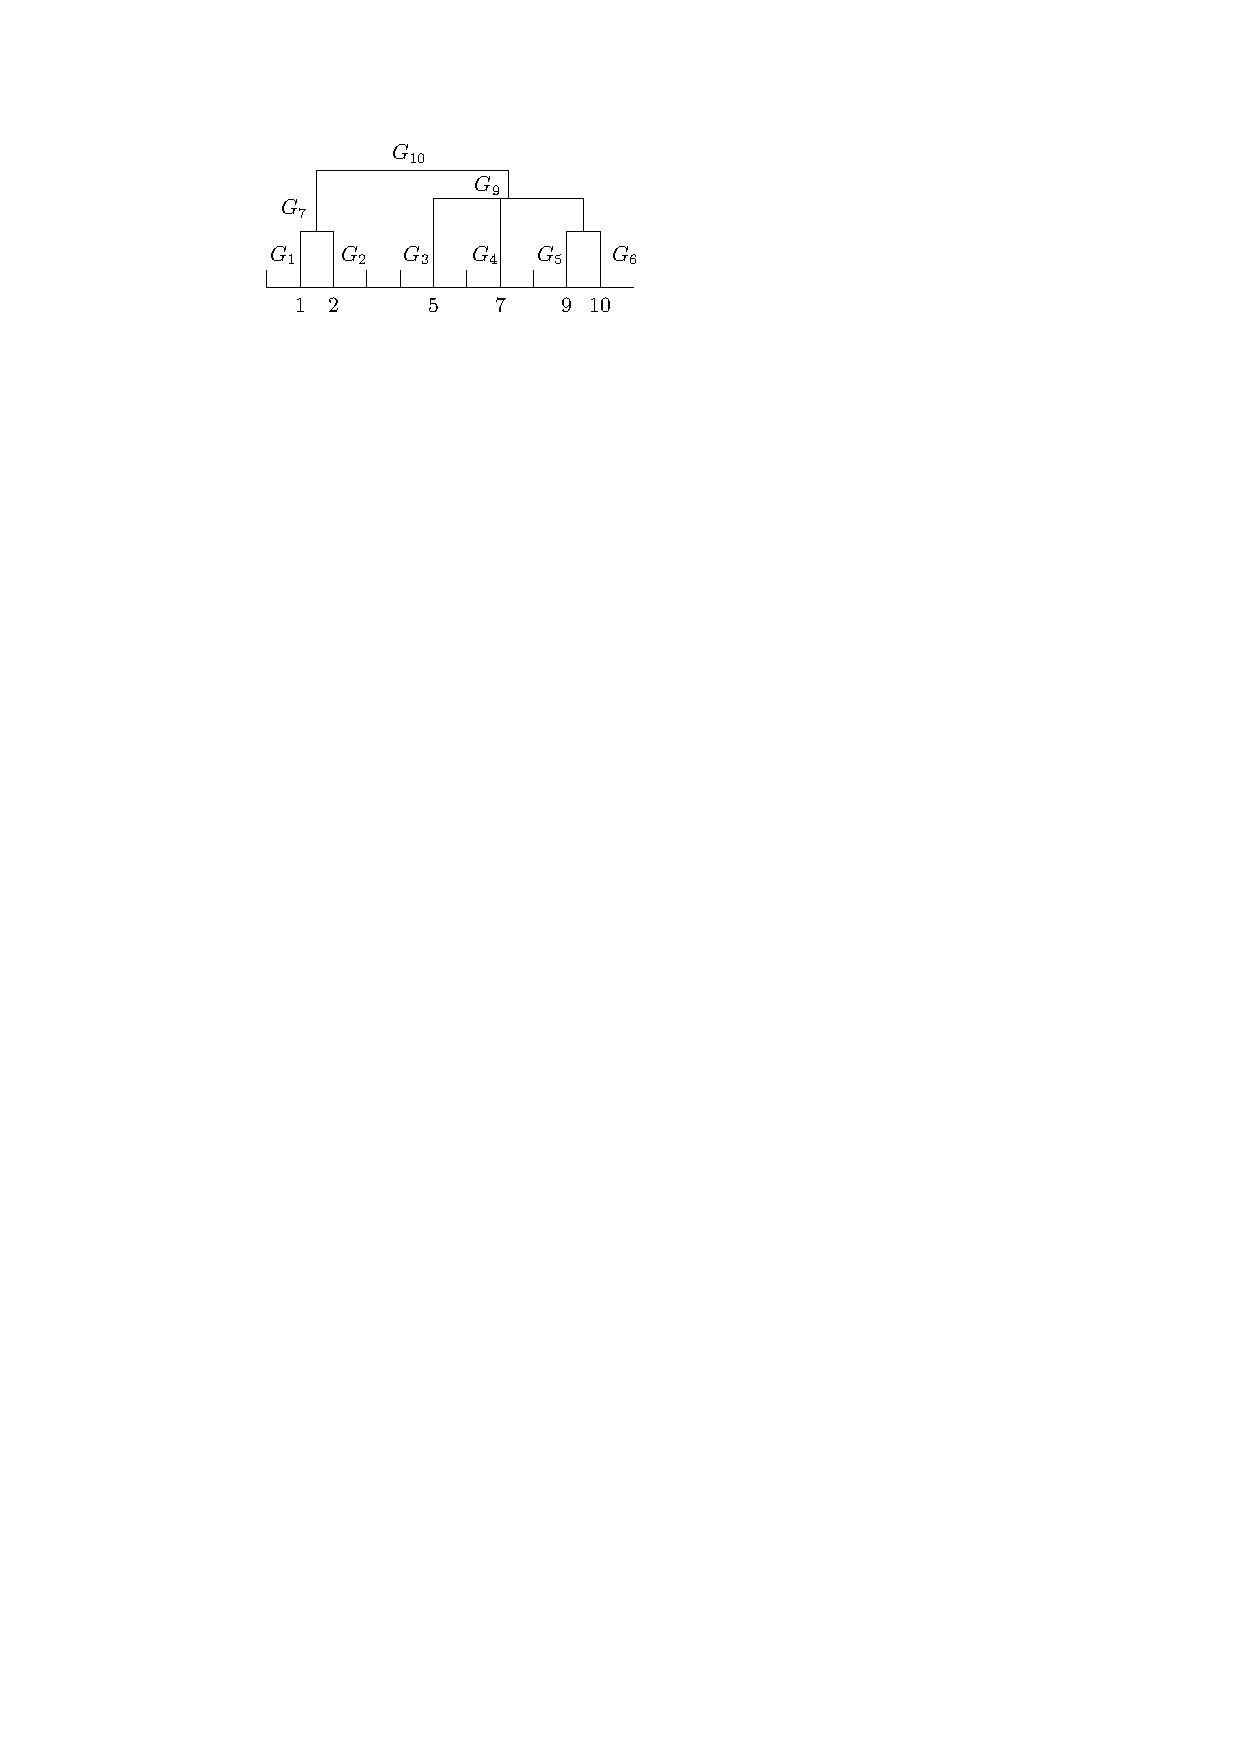
\includegraphics{image/层次聚类举例可视化.pdf}
        \end{figure}
    \end{enumerate}
\end{example}
\begin{note}
    层次聚类的优缺点:
    \begin{itemize}
        \item 优点
        \begin{itemize}
            \item 不需要预先设定聚类数
            \item 可以发现簇的层次关系
            \item 可以聚类成除球形簇之外的其它形状
        \end{itemize}
        \item 缺点
        \begin{itemize}
            \item 计算复杂度高
            \item 对离群点敏感
            \item 可能聚成链状
        \end{itemize}
    \end{itemize}
\end{note}
\subsection{人工神经网络}
\subsubsection{生物神经元与神经网络}
神经元是神经系统结构与功能的基本单元。
\begin{figure}[htbp]
    \centering
    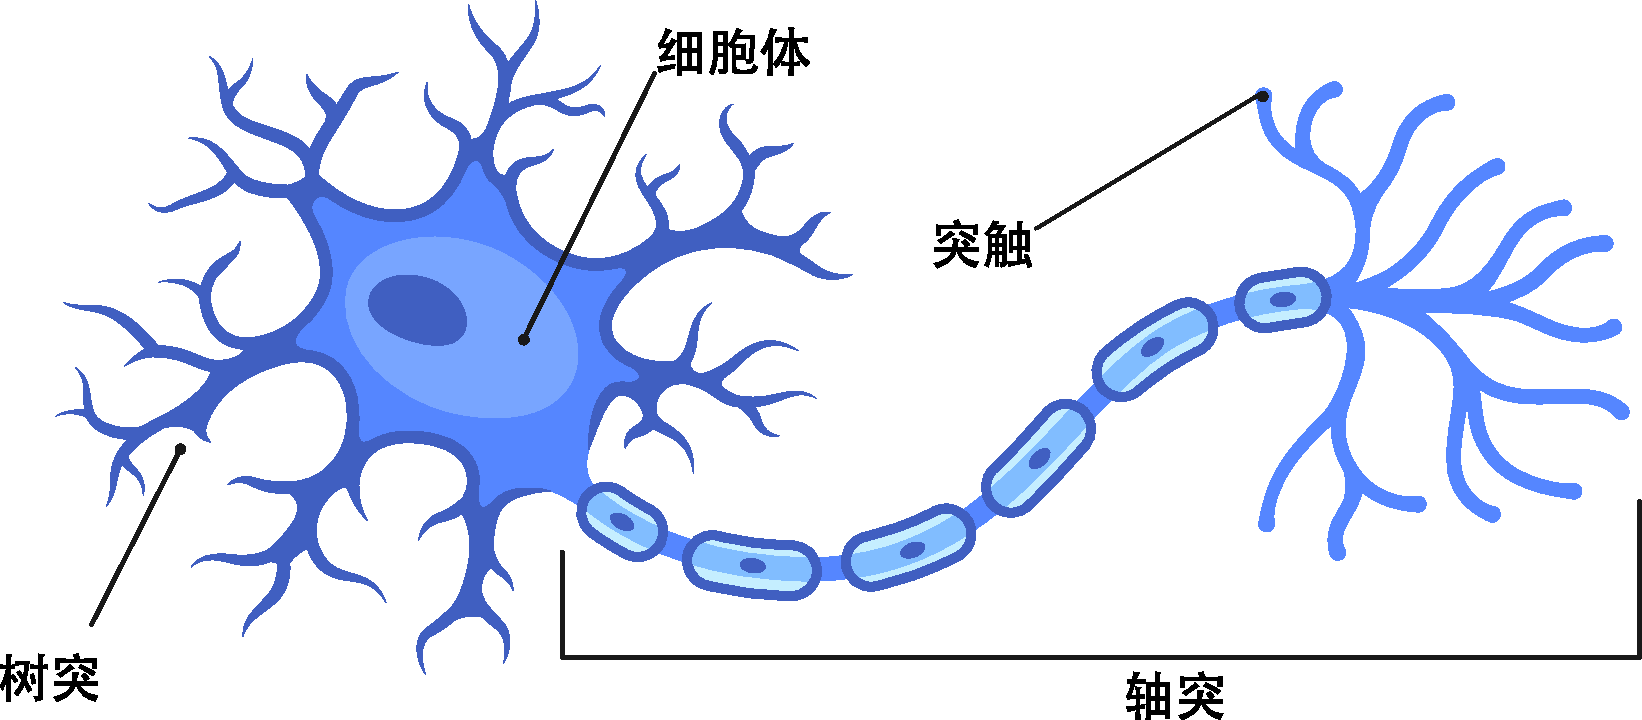
\includegraphics[width = .5\textwidth]{image/NeuronFreeVectorIllustration.pdf}
\end{figure}
\begin{itemize}
    \item 树突:神经纤维接收器,将电信号传送到细胞体
    \item 细胞体:对输入信号进行整合和阈值处理
    \item 轴突:把细胞体的输出信号导向其他神经元
    \item 突触:一个神经细胞的轴突和另一个神经细胞树突的结合点
\end{itemize}
\begin{note}
    生物神经元的信息处理过程:
    \begin{itemize}
        \item 信息输入
        \item 空间整合:同一时刻产生的刺激所引起的膜电位变化,大致等于各单独刺激引起的膜电位变化的代数和。
        \item 时间整合:各输入脉冲抵达神经元的时间先后不一样。总的突触后膜电位为一段时间内的累积。
        \item 信息产生
        \item 信息传导
        \item 兴奋或抑制
    \end{itemize}
    小结:树突从细胞体伸向其它神经元,神经元之间通过突触连接。通过突触输入的信号起着兴奋 抑制作用。当细胞体接受的累加兴奋作用超过某阈值时,细胞进入兴奋状态,产生冲动,并由轴突输出。
\end{note}
\begin{note}
    生物神经元的基本特点:
    \begin{itemize}
        \item 神经元传递信息过程为多输入、单输出;
        \item 输入信号可以起兴奋作用,也可以起抑制作用;
        \item 神经元之间的连接强度可以随训练而改变,并决定信号传递的强弱;
        \item 每个神经元有一个“阈值”,一个神经元接受信号的累积效果决定该神经元的状态。
    \end{itemize}
\end{note}
\begin{example}
    生物神经元基本特点不包括:    
    \begin{enumerate}[A]
        \item 多输入单输出
        \item 时空整合功能
        \item \textcolor{main1}{兴奋性}
        \item 阈值特性
    \end{enumerate}
\end{example}
\begin{example}
    生物神经网络是如何实现信息的记忆和分布存储的? 
    \begin{enumerate}[A]
        \item 大脑里有类似于硬盘的存储脑区
        \item \textcolor{main1}{通过突触连接强度的改变进行存储}
    \end{enumerate}
\end{example}
\subsubsection{人工神经网络三大要素}
\textcolor{main1}{人工神经网络三大要素}
\begin{itemize}
    \item 神经元特性
    \item 网络结构
    \item 学习规则/学习算法
\end{itemize}

\textcolor{main1}{一、人工神经元数理模型}
\begin{figure}[htbp]
    \centering
    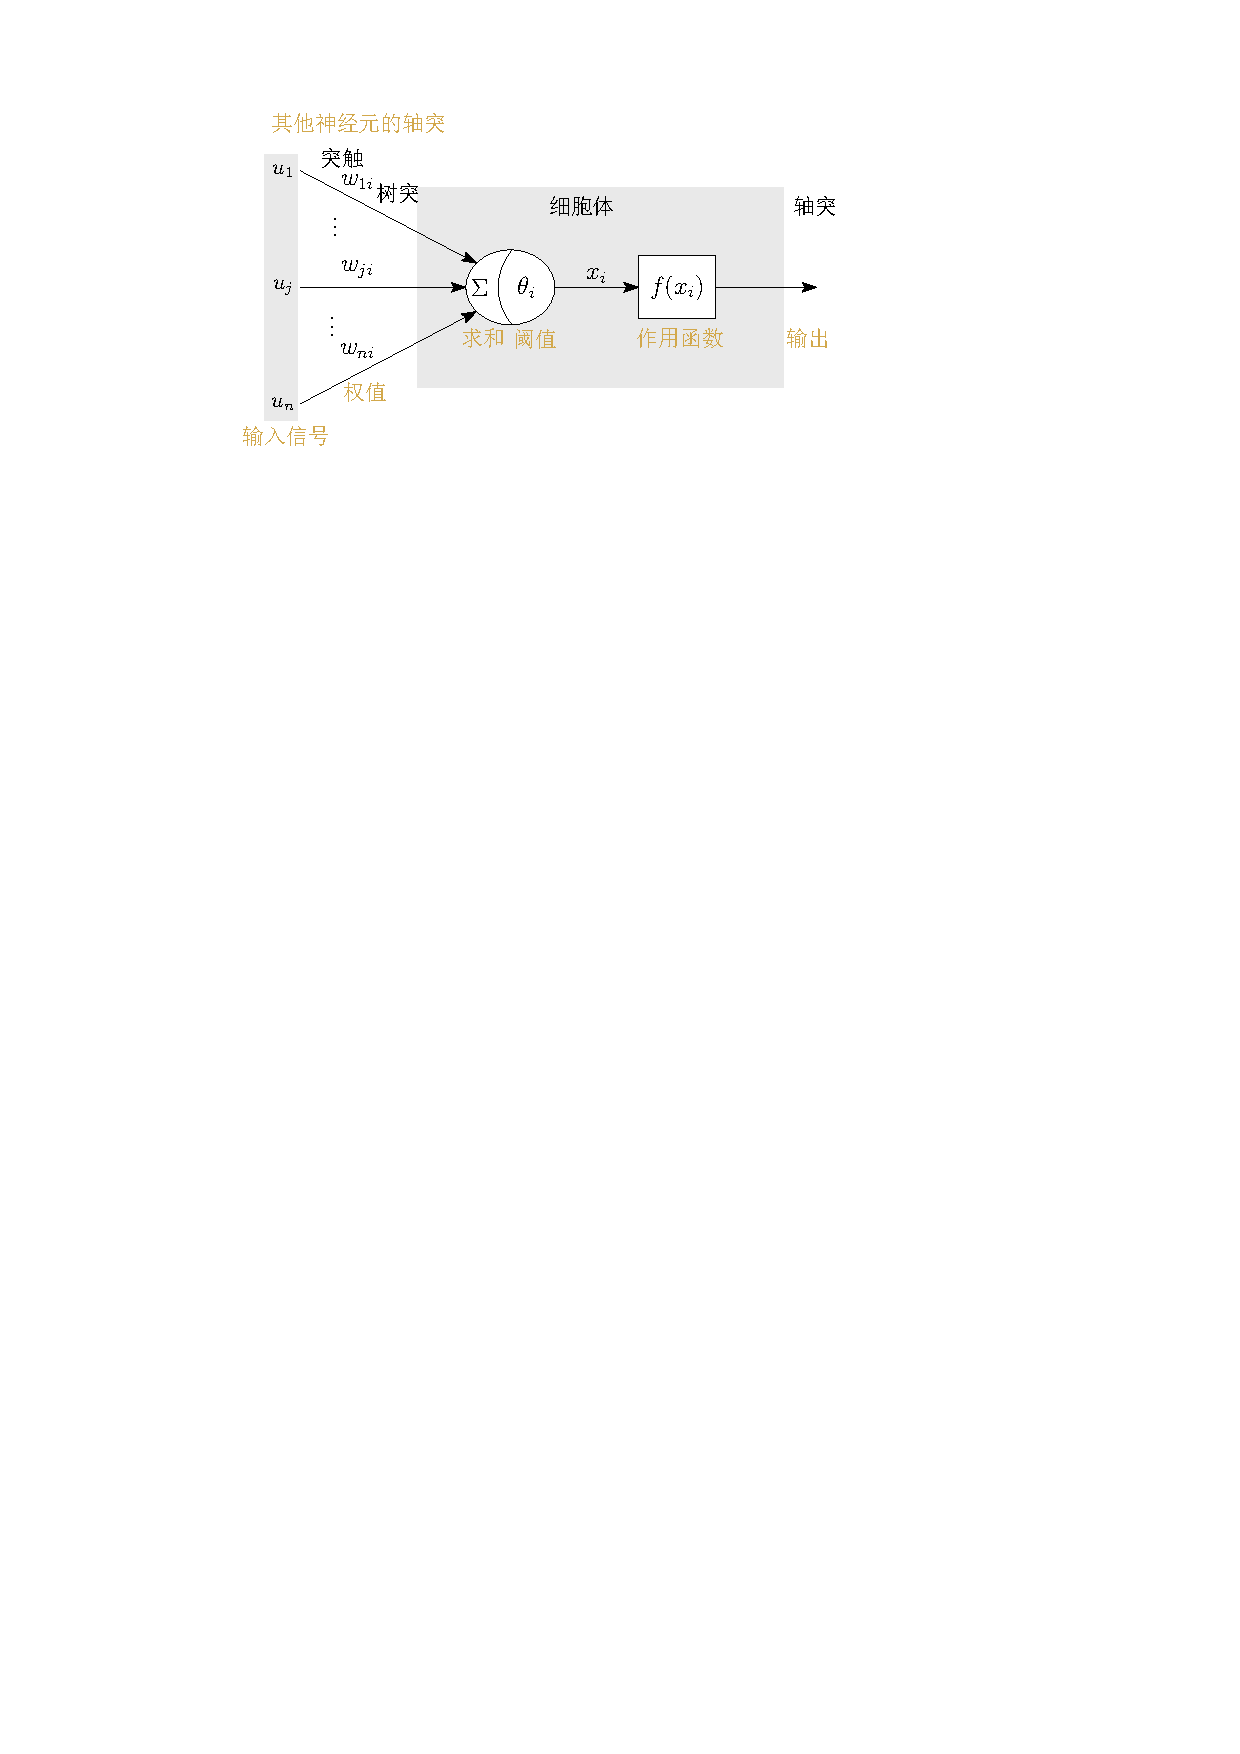
\includegraphics{image/MP神经元模型.pdf}
\end{figure}
\begin{itemize}
    \item 求和操作 $x_i = \sum\limits_{j = 1}^{n}w_{ji}u_{j}-\theta_{i}$
    \item 作用函数 $y_i = f(x_i) = f\left( \sum\limits_{j = 1}^{n}w_{ji}u_{j}-\theta_{i} \right)$
    \begin{itemize}
        \item 作用函数控制输入对输出的激活作用
        \item 作用函数对输入、输出进行函数转换
        \item 作用函数将无限域的输入变换成有限范围内的输出
    \end{itemize}
    \item MP神经元模型中的作用函数为单位阶跃函数:
    \[
        f(x) = \left\{
            \begin{array}{ll}
                1, & x\geq 0\\
                0, & x<0
            \end{array}
        \right.
    \]
    当神经元$i $的输入信号加权和超过阈值时,输出为“1”,即“兴奋”状态;反之输出为“0”,是“抑制”状态。
\end{itemize}
\begin{example}
    给定神经元的结构和权值,采用单位阶跃函数作为作用函数,对于不同的输入,分别计算神经元的输出。
    \begin{figure}[htbp]
        \centering
        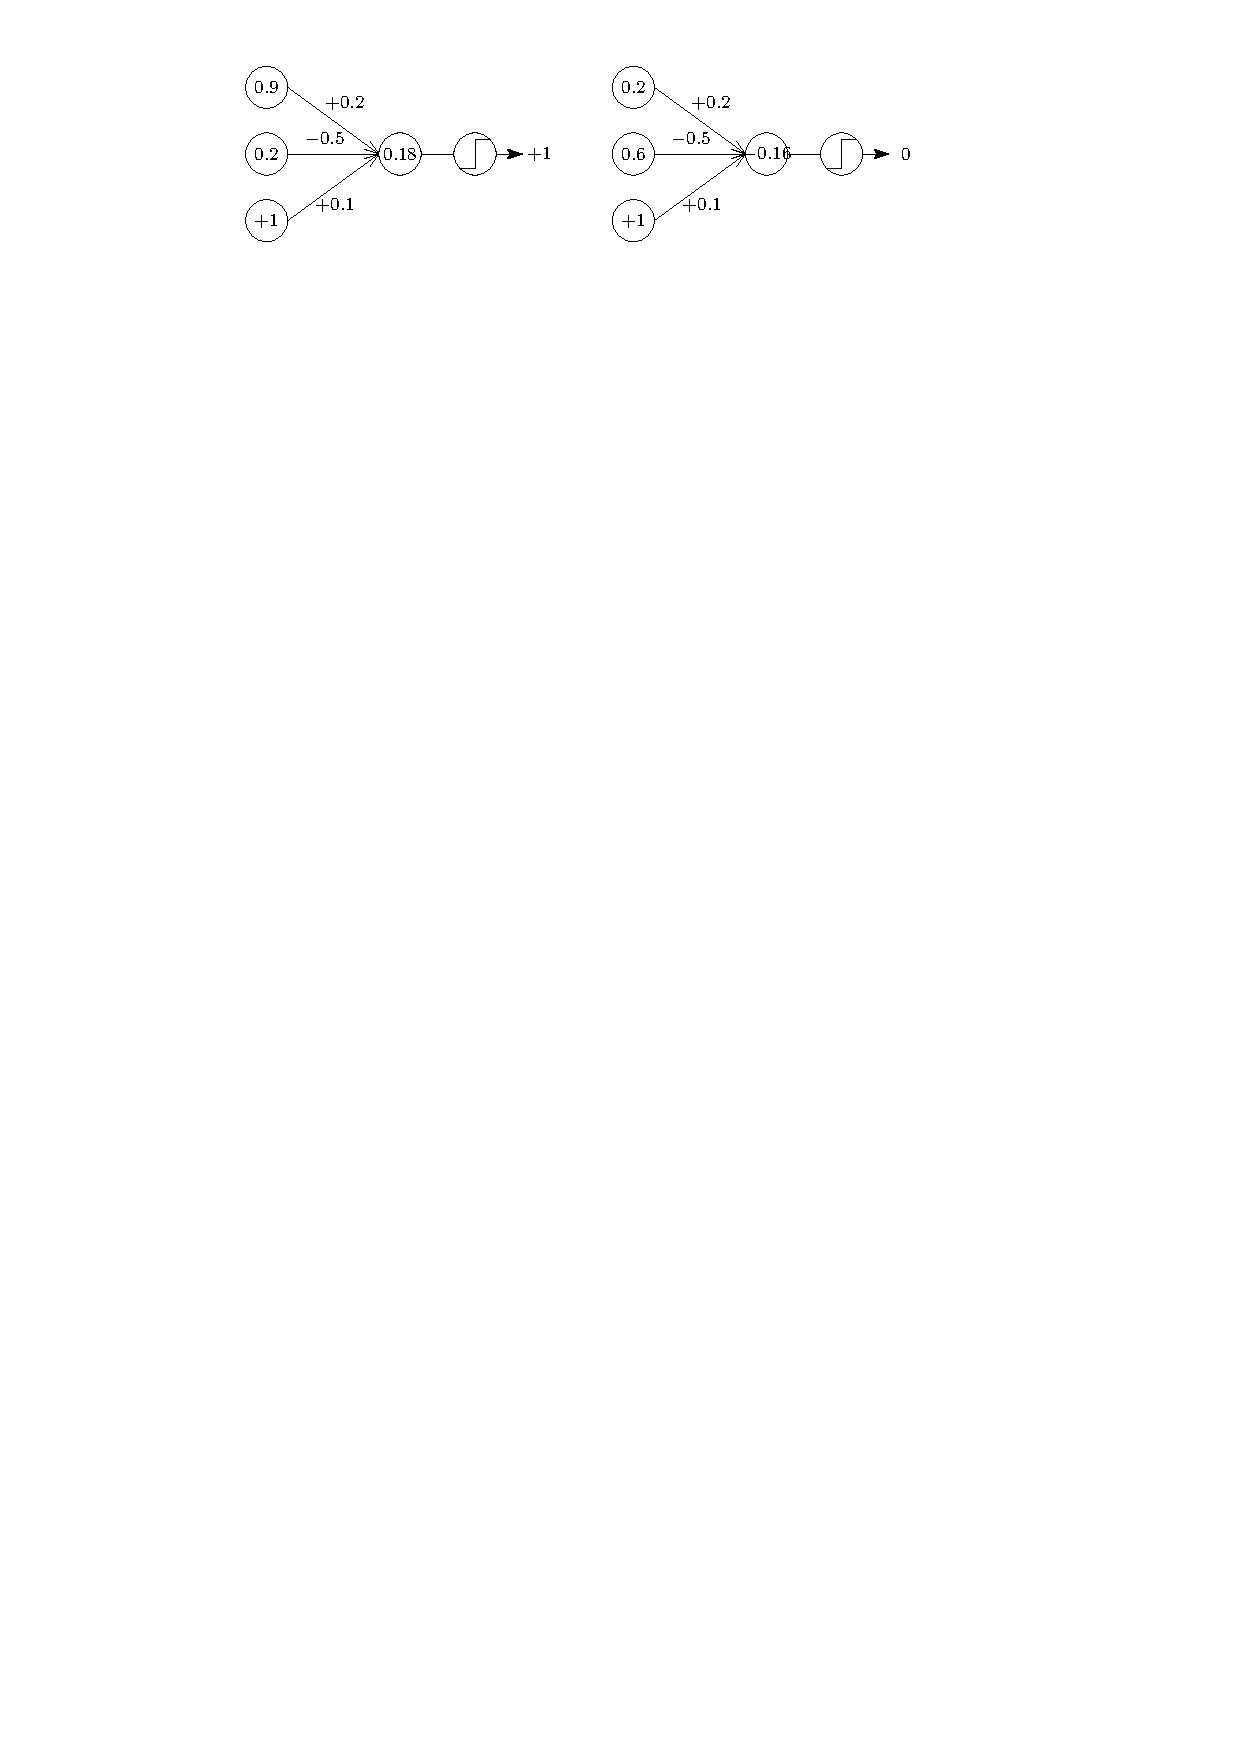
\includegraphics{image/计算MP神经元的输出.pdf}
    \end{figure}
\end{example}
\textcolor{main1}{常见的神经元作用函数}

神经元的作用函数反映了神经元输出与其激活状态之间的关系。神经元的各种数学模型的主要区别在于采用了不同的作用函数,从而使神经元具有不同的信息处理特性。
\begin{itemize}
    \item 阈值型
    
    \textcolor{main1}{采用阶跃作用函数的神经元,称为阈值逻辑单元}
    \begin{figure}[htbp]
        \centering
        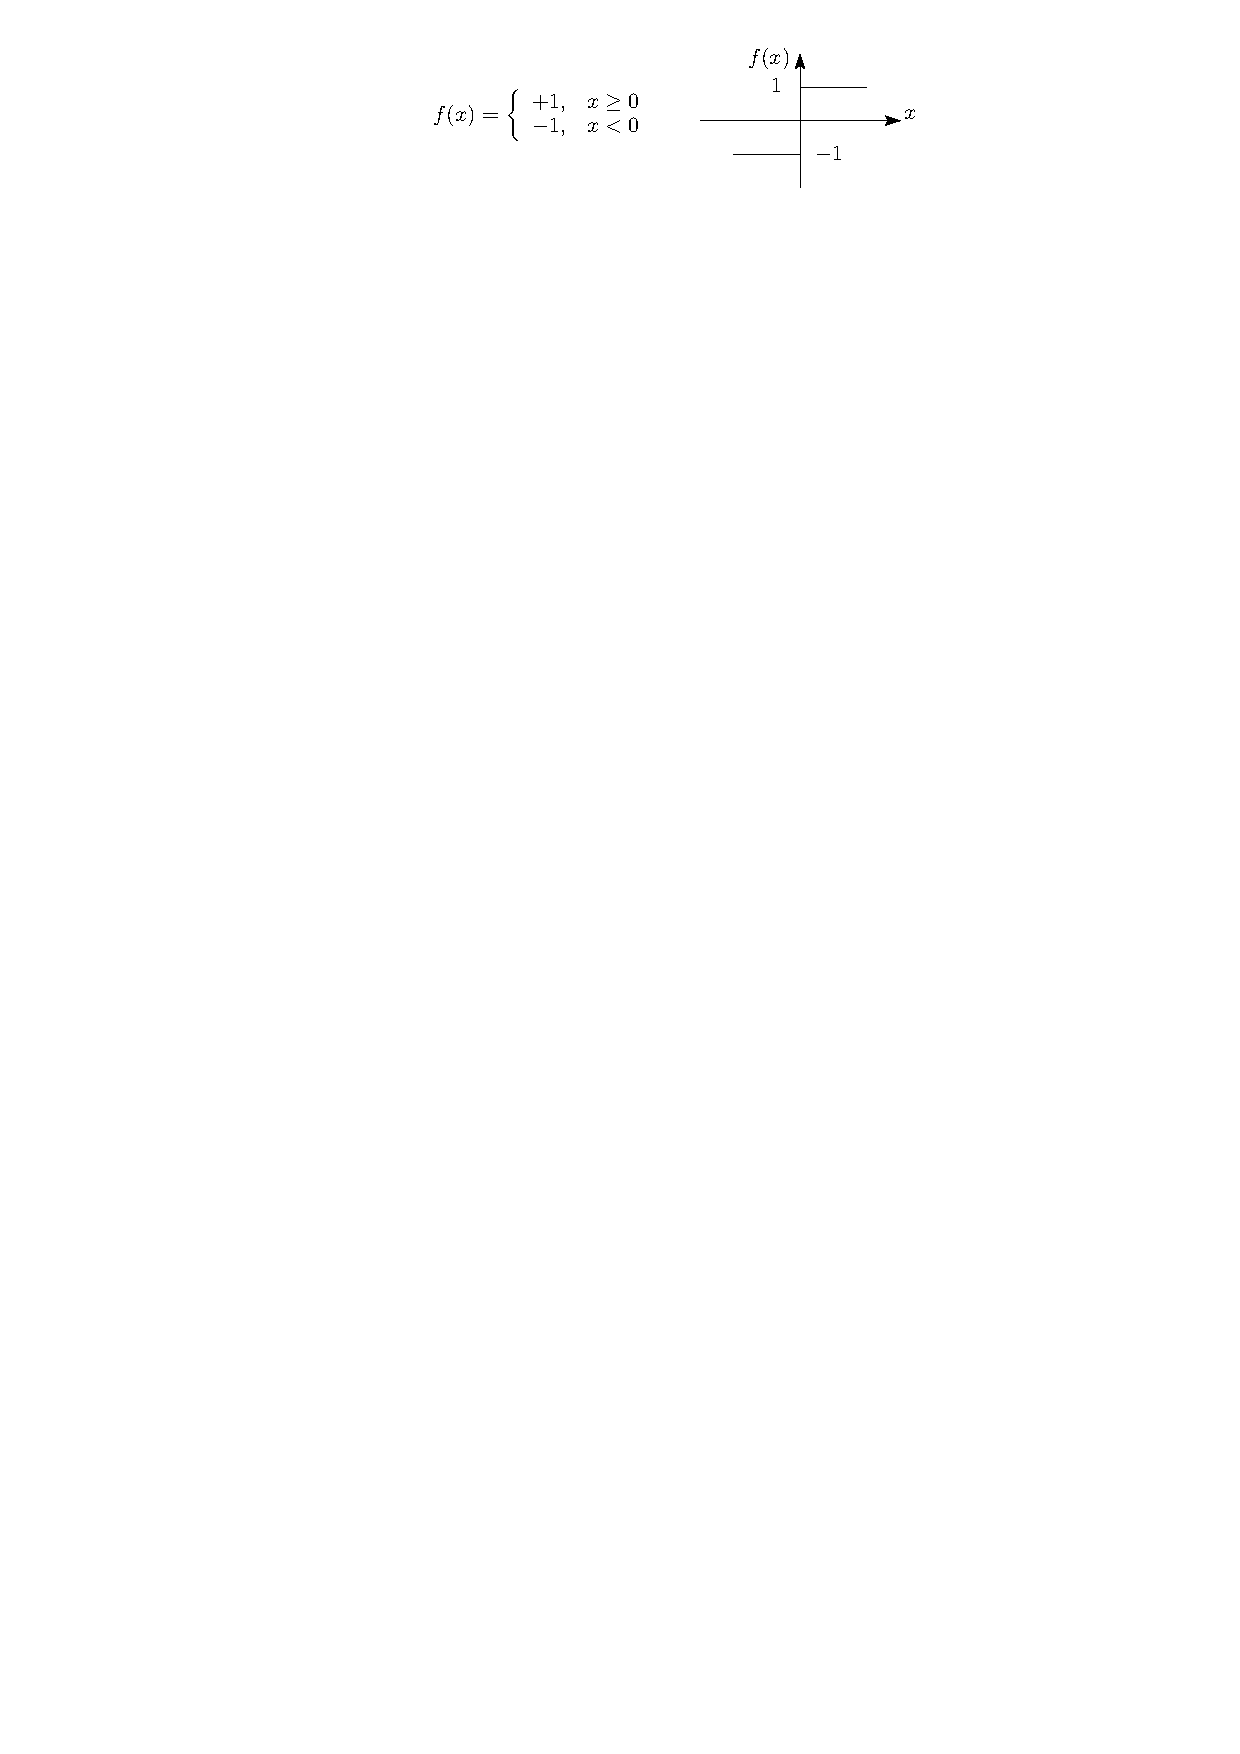
\includegraphics{image/阈值型f.pdf}
    \end{figure}
    \item 连续非线性作用函数
    \begin{figure}[htbp]
        \centering
        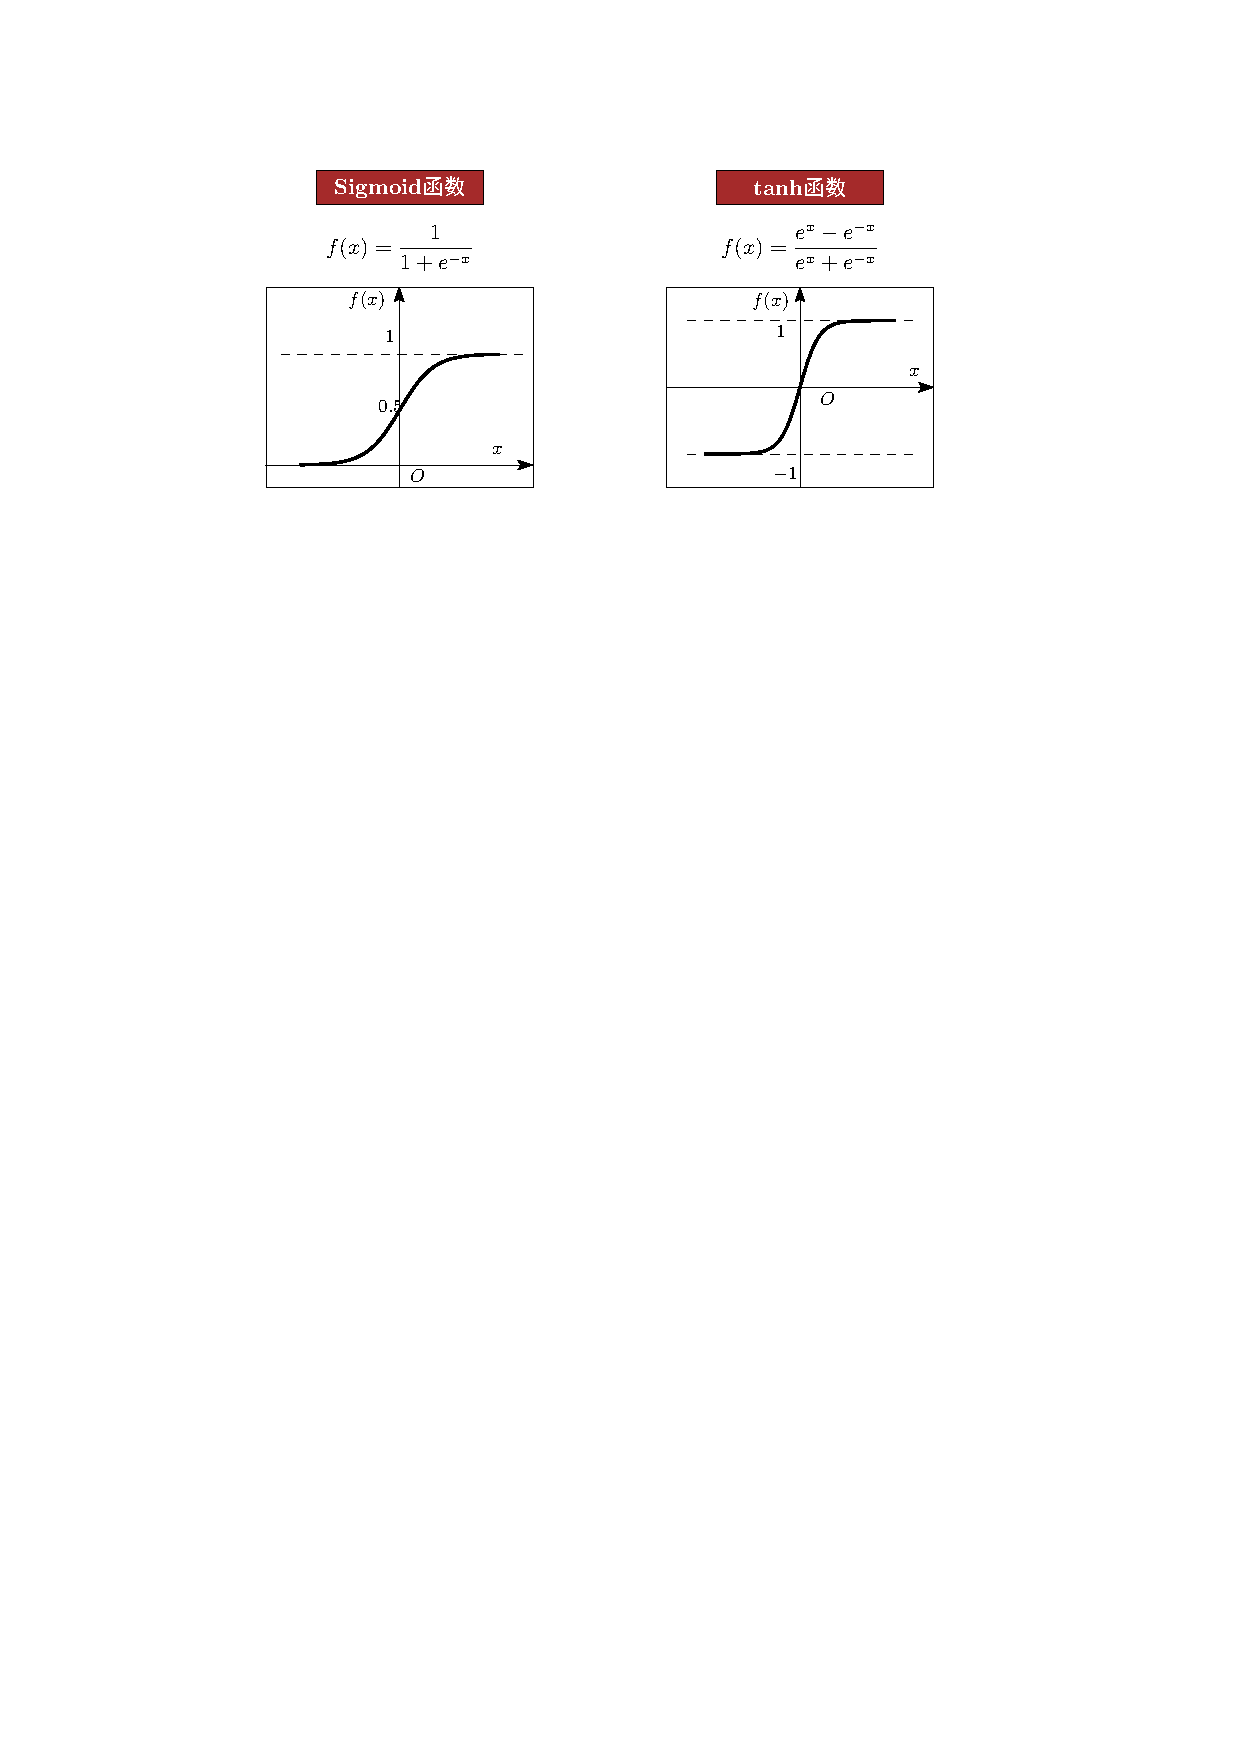
\includegraphics{image/连续非线性作用函数.pdf}
    \end{figure}
    
    \item 分段线性作用函数
    \begin{figure}[htbp]
        \centering
        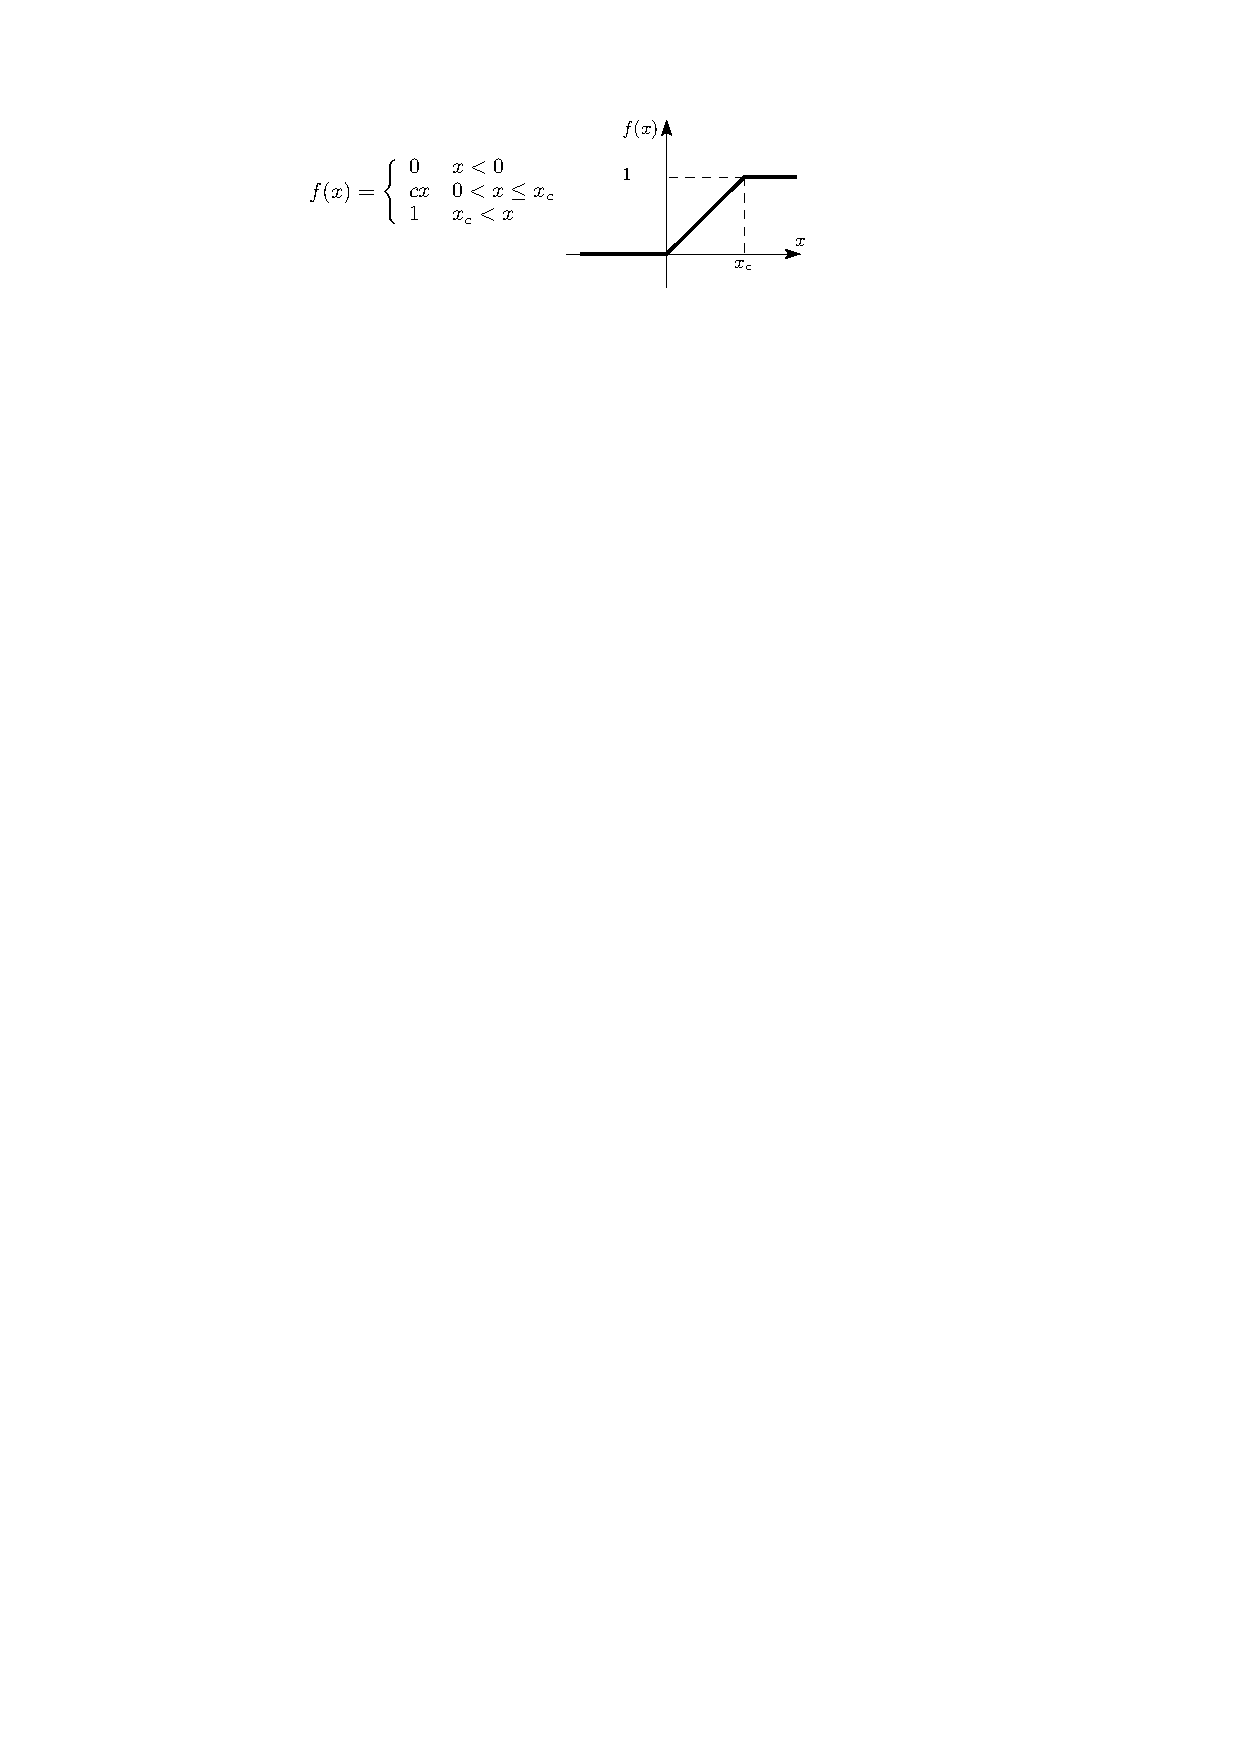
\includegraphics{image/分段线性作用函数.pdf}
    \end{figure}
\end{itemize}
\textcolor{main1}{人工神经元特性与生物神经元特性的比较}
    % Table generated by Excel2LaTeX from sheet '人工神经元特性与生物神经元特性的比较'
    \begin{table}[H]
        \centering
        \small{
        \begin{tabular}{cc}
        \toprule[1.5pt]
        生物神经元 & 人工神经元 \\
        \midrule[1pt]
        多输入单输出 & $[u_1 ,u_2 ,\dots,u_n]$ 到$y_i$ 的映射 \\
        信号分兴奋和抑制 & 输出值的正负对应兴奋和抑制 \\
        连接强度决定信号传递强弱 & $w_{ji} $值为输入$u_j$ 提供权值 \\
        连接强度可变 & $w_{ji} $值可随训练改变 \\
        每个神经元有一个阈值 & 阈值$\theta_{i}$表现阈值特性 \\
        信号累加效应决定神经元状态 & 净输入$x_i$表现空间整合特性 \\
        \bottomrule[1.5pt]
        \end{tabular}%
        }
    \end{table}%
  
\begin{example}
    关于作用函数的基本作用不正确的是:
    \begin{enumerate}[A]
        \item 控制输入对输出的激活作用
        \item \textcolor{main1}{决定信号传递强弱}
        \item 对输入、输出进行函数转换
        \item 将可能无限域的输入变换成指定的有限范围内的输出
    \end{enumerate}
\end{example}

\textcolor{main1}{二、人工神经网络结构}

\begin{note}
    人工神经网络结构的分类:
    \begin{itemize}
        \item 神经网络强大的计算功能是通过神经元的互连而达到的。根据网络拓扑结构形式不同,人工神经网络分为\textcolor{main1}{层次型神经网络}和\textcolor{main1}{互连型神经网络}。
        \item 如果从神经网络内部信息传递方向来看,人工神经网络可分为\textcolor{main1}{前馈型神经网络}和\textcolor{main1}{反馈型神经网络}。
    \end{itemize}
\end{note}
\begin{note}
    层次型神经网络
    \begin{itemize}
        \item 单纯型(前向神经网络):神经元分层排列,顺序连接,神经元之间不存在反馈。如感知器、BP 神经网络等。
        \begin{figure}[htbp]
            \centering
            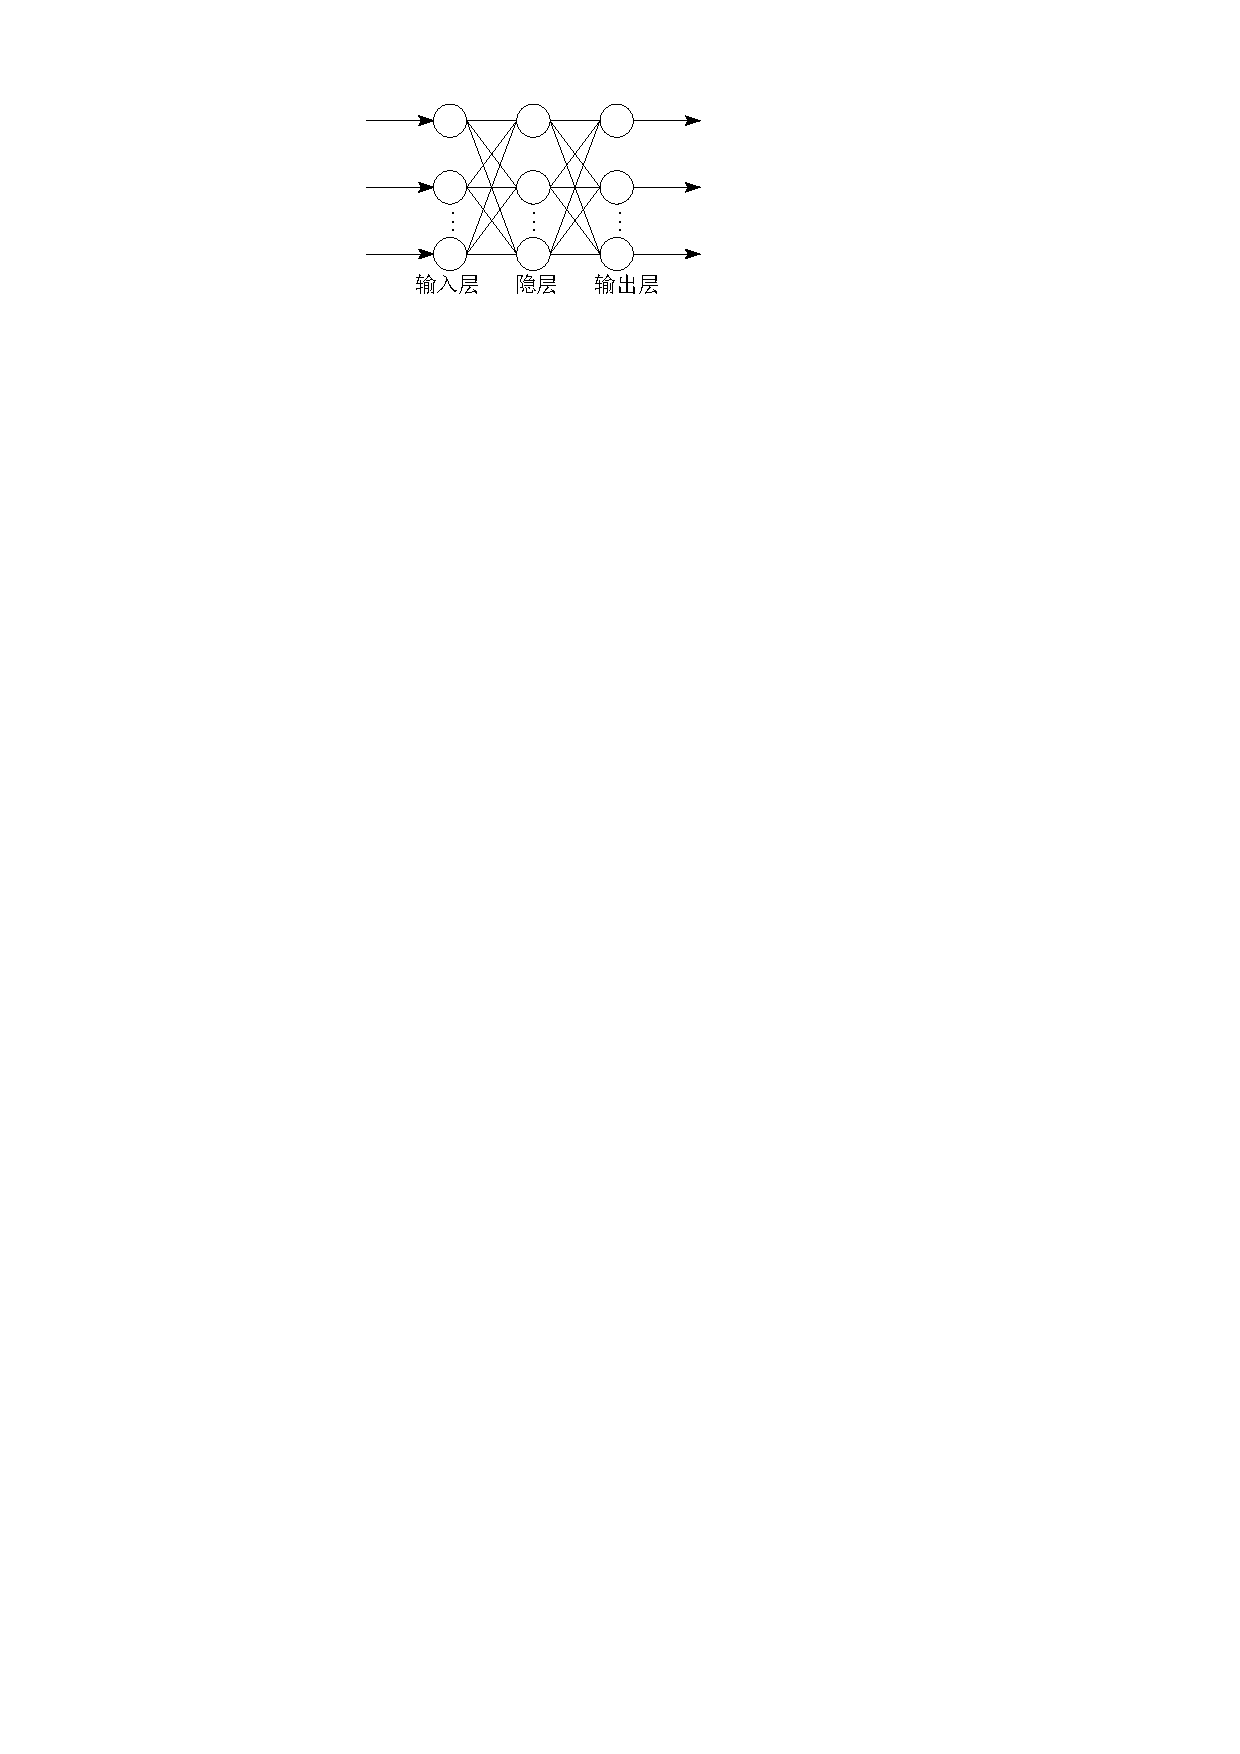
\includegraphics{image/单纯型.pdf}
        \end{figure}
        \item 层内有互连型:层内神经元相互连接,实现同层内神经元间的横向抑制或兴奋机制,以实现各层神经元的自组织。
        \begin{figure}[htbp]
            \centering
            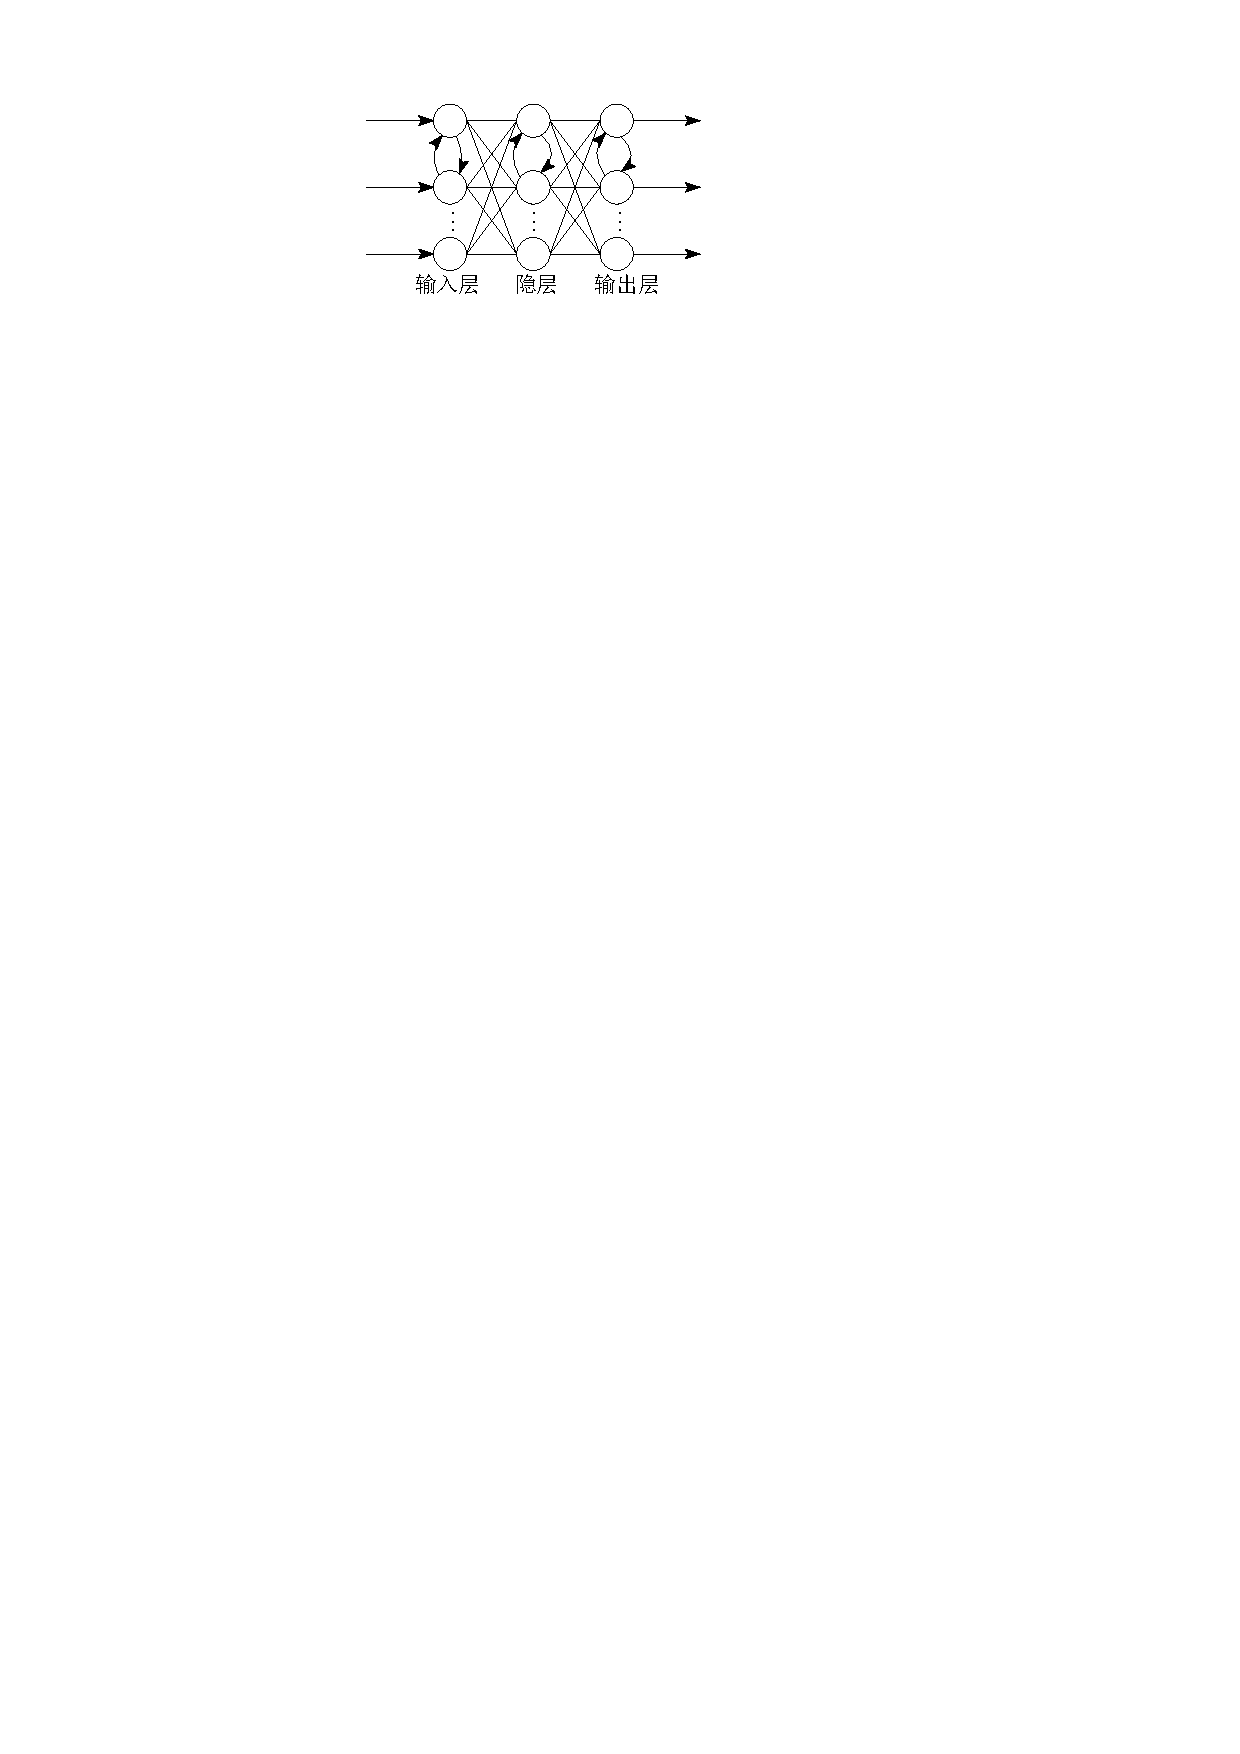
\includegraphics{image/层内有互连型.pdf}
        \end{figure}
        \item 有反馈型:输出由当前输入和先前输出共同决定,类似于人类短期记忆。
        \begin{figure}[htbp]
            \centering
            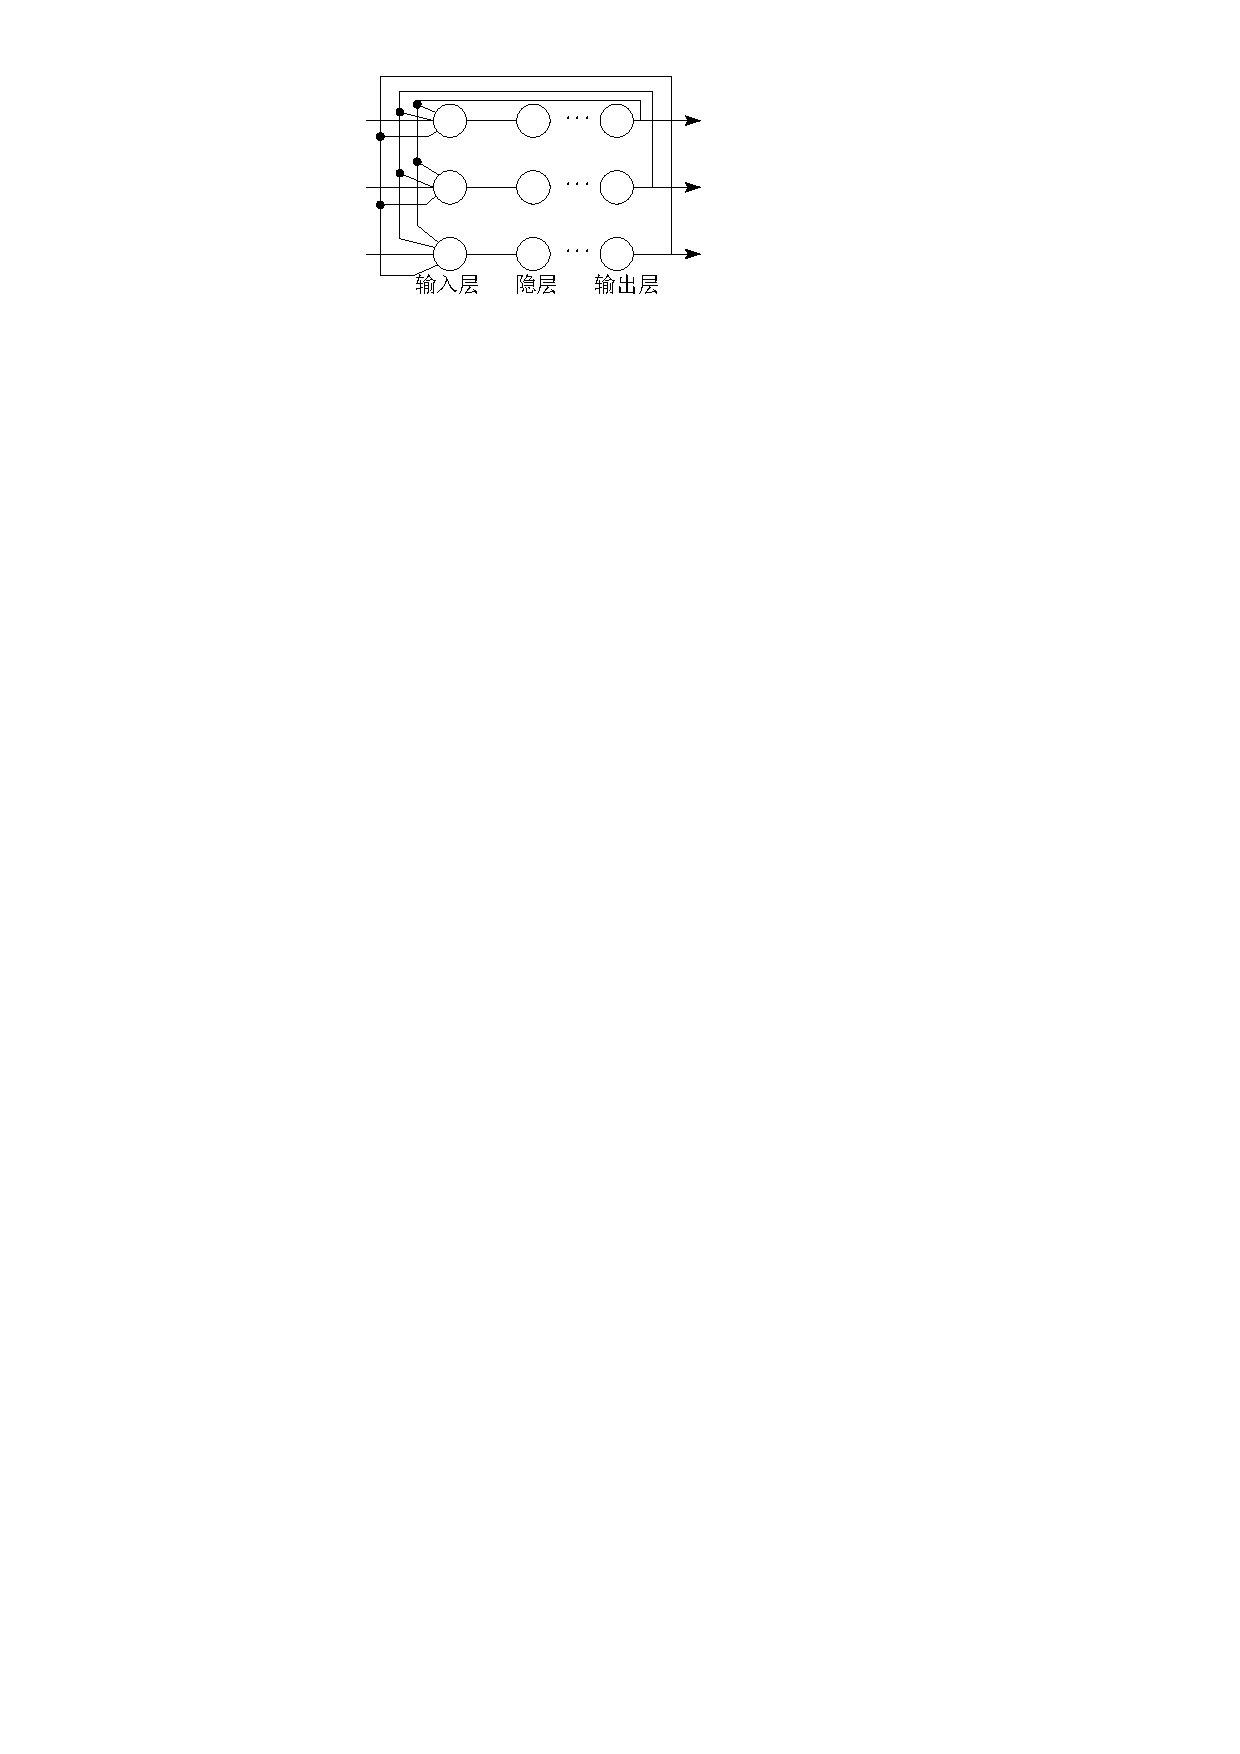
\includegraphics{image/有反馈型.pdf}
        \end{figure}
    \end{itemize}
\end{note}
\begin{definition}[互连型神经网络]
    任意两个神经元之间都可能有相互连接。有的神经元之间的连接是双向的,有的是单向的。如Hopfield 网络、Boltzman 机网络。
    \begin{figure}[htbp]
        \centering
        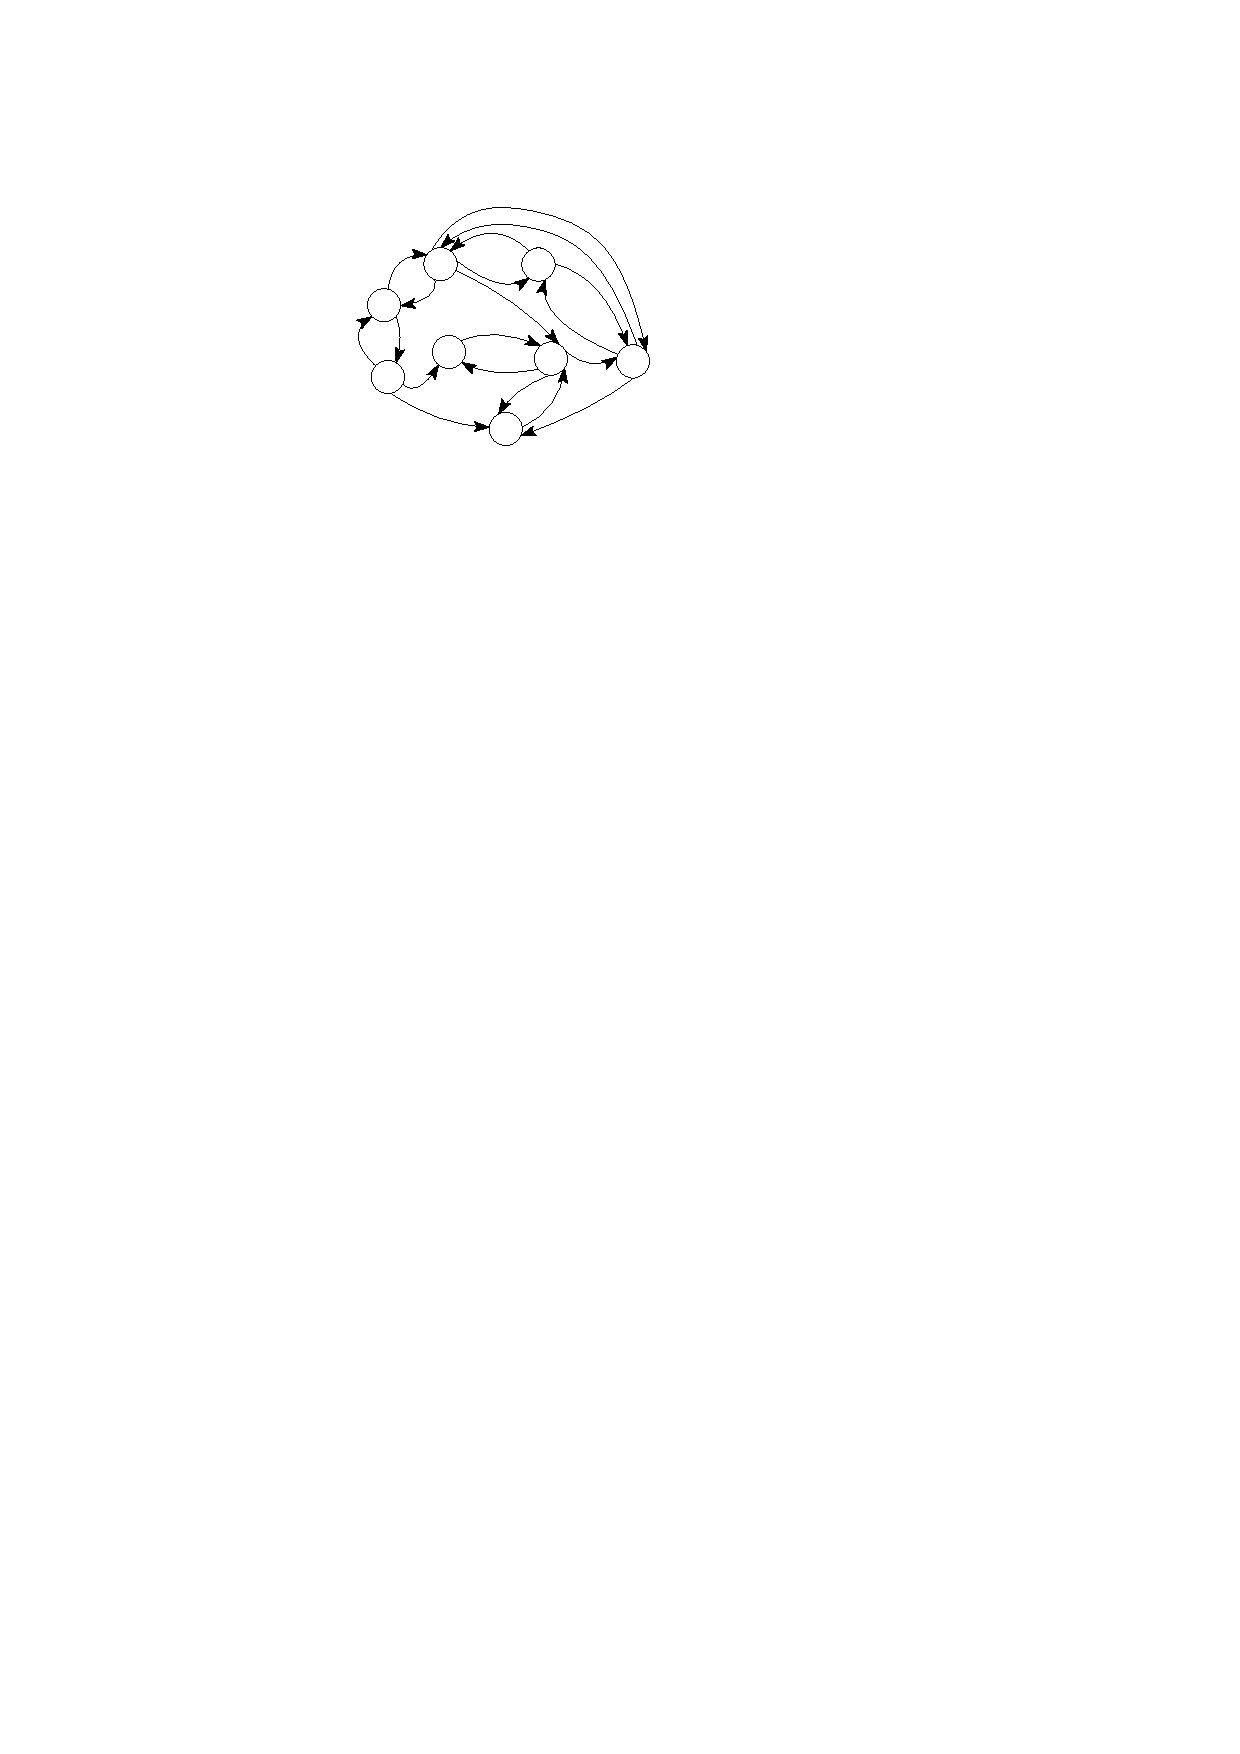
\includegraphics{image/互连型神经网络.pdf}
    \end{figure}
\end{definition}
\begin{note}
    无反馈的前向网络和互连型网络:
    \begin{itemize}
        \item 在无反馈的前向网络中,信号一旦通过某个神经元,过程就结束了。
        \item 在互连型网络中,信号在神经元之间反复往返传递,网络处在不断改变状态的动态中。从初始状态开始,经过若干次变化,到达某平衡状态或进入周期振荡。
    \end{itemize}
\end{note}
\begin{note}
    人工神经网络结构的比较:
    \begin{itemize}
        \item 前馈型神经网络
        
        网络中各神经元接受前一层的输入,并输出到下一层,没有反馈。可实现信号从输入空间到输出空间的变换,信息处理能力来自于简单非线性函数的多次整合。网络结构简单,易于实现。适合于解决一般的函数逼近和预测问题。
        \item 反馈型神经网络
        
        网络中神经元间有反馈,信息处理体现为状态的变换,可以用动力学系统描述。系统的稳定性与联想记忆功能有密切关系。适合于解决动态序列分析或联想记忆等问题。
    \end{itemize}
\end{note}

\textcolor{main1}{三、学习算法}
\begin{note}
    神经网络的运行阶段
    \begin{itemize}
        \item 学习阶段:也称自适应期或设计期,通过学习训练样本或其他方法调整权值矩阵;
        \item 工作阶段:各连接权值不再改变,用于求解实际问题。
    \end{itemize}
\end{note}
\begin{itemize}
    \item 学习的目的是从训练数据中提取隐含的知识和规律,并存储于网络中供工作阶段使用。
    \item 学习是改变各神经元连接权值的有效方法,也是体现人工神经网络智能特性最主要的标志。离开了学习,神经网络就失去了诱人的自适应、自组织能力。
\end{itemize}
\begin{note}
    \textcolor{main1}{神经网路的学习方式}
    \begin{itemize}
        \item 有监督学习
        
        根据实际输出与期望输出的偏差,按照一定的准则调整各神经元连接权值。期望输出是评价学习的标准,又称为有导师学习。
        \item 无监督学习
        
        神经网络仅根据其输入调整权值,网络的学习评价标准隐含于内部。
    \end{itemize}
\end{note}
\begin{note}
    神经网络的学习规则:Delta($\delta$) 学习规则
    \begin{itemize}
        \item 对于输入$u$,期望输出$d$,实际输出与期望输出之间存在着误差$e$
        \[
            e = d - y
        \]
        \item 调整权值,使误差$e$减小到一定范围,设置目标函数
        \[
            E = \frac{1}{2}e^2
        \]
        该学习过程称为纠错学习,或Delta学习规则。
        \item 平方误差
        \[
            E = \frac{1}{2}\left( d-y(t) \right)^2 = \frac{1}{2}\left( d-f\left( \boldsymbol{W}^{\mathrm{T}}(t)\boldsymbol{U} \right) \right)^2
        \]
        \item 沿着\textcolor{main1}{负梯度方向}调整权值
        \[
            \begin{array}{ll}
                \Delta \boldsymbol{W}(t) &= -\eta \nabla E\\
                &=\eta \left( d-y(t) \right)f'\left( x(t) \right)\boldsymbol{U}
            \end{array}
        \]
    \end{itemize}
\end{note}
\begin{example}
    对于四输入单输出神经元 设作用函数为双极性Sigmod 函数,学习率$\eta = 0.1$,输出为$\boldsymbol{U}_1 = \begin{bmatrix}
        -1 & 1 & -2 &0
    \end{bmatrix}^{\mathrm{T}},\,\boldsymbol{U}_2 = \begin{bmatrix}
        -1 & 0 & 1.5 & -0.5
    \end{bmatrix}^{\mathrm{T}},\,\boldsymbol{U}_3 = \begin{bmatrix}
        -1 & -1 & 1 & 0.5
    \end{bmatrix}^{\mathrm{T}}$,权值初始值为$\boldsymbol{W}(0) = \begin{bmatrix}
        0.5 & 1 & -1 & 0
    \end{bmatrix}^{\mathrm{T}}$,期望输出为$d_1 = -1,\,d_2 = -1,\, d_3 = 1$,试按照$\delta$规则进行网络学习。

    \textcolor{main1}{解:}已知作用函数为$f(x) = \dfrac{1-e^{-x}}{1+e^{-x}}$,则
    \[
        f'(x) = \dfrac{2e^{-x}}{\left( 1+e^{-x} \right)^2},\,f'(x) = \dfrac{1}{2}\left[ 1-f(x)^2 \right]
    \]
    \begin{enumerate}
        \item 输入$\boldsymbol{U}_1$,计算净输入$x_{1}$及权向量$\boldsymbol{W}(1)$
        \[
            \begin{array}{l}
                x_1 = \boldsymbol{W}^{\mathrm{T}}(0)\boldsymbol{U}_1 = 2.5,\, y_{1} = f(x_1) = 0.848\\
                f'(x_1) = \dfrac{1}{2}(1-y_1^2) = 0.140\\
                \boldsymbol{W}(1) = \begin{bmatrix}
                    0.526 & 0.974 & -0.948 & 0 
                \end{bmatrix}^{\mathrm{T}}
            \end{array}
        \]
        \item 输入$\boldsymbol{U}_2$,计算净输入$x_{2}$及权向量$\boldsymbol{W}(2)$
        \[
            \begin{array}{l}
                x_2 = \boldsymbol{W}^{\mathrm{T}}(1)\boldsymbol{U}_2 = -1.948,\, y_{2} = f(x_2) = -0.75\\
                f'(x_2) = \dfrac{1}{2}(1-y_2^2) = 0.218\\
                \boldsymbol{W}(2) = \begin{bmatrix}
                    0.531 & 0.974 & -0.956 & 0.002
                \end{bmatrix}^{\mathrm{T}}
            \end{array}
        \]
        \item 输入$\boldsymbol{U}_3$,计算净输入$x_{3}$及权向量$\boldsymbol{W}(3)$
        \[
            \begin{array}{l}
                x_3 = \boldsymbol{W}^{\mathrm{T}}(2)\boldsymbol{U}_3 = -2.46,\, y_{3} = f(x_3) = -0.842\\
                f'(x_3) = \dfrac{1}{2}(1-y_3^2) = 0.145\\
                \boldsymbol{W}(3) = \begin{bmatrix}
                    0.505 & 0.947 & -0.929 & 0.016
                \end{bmatrix}^{\mathrm{T}}
            \end{array}
        \]
    \end{enumerate}
\end{example}
\begin{note}
    Delta($\delta$)学习规则的特点
    \begin{itemize}
        \item $\delta$规则要求\textcolor{main1}{作用函数可导},适用于有监督学习的连续作用函数,如Sigmoid 函数。可推广到多层前向网络,权值可初始化为任意值。
    \end{itemize}
\end{note}
\subsubsection{感知器}
\begin{figure}[htbp]
    \centering
    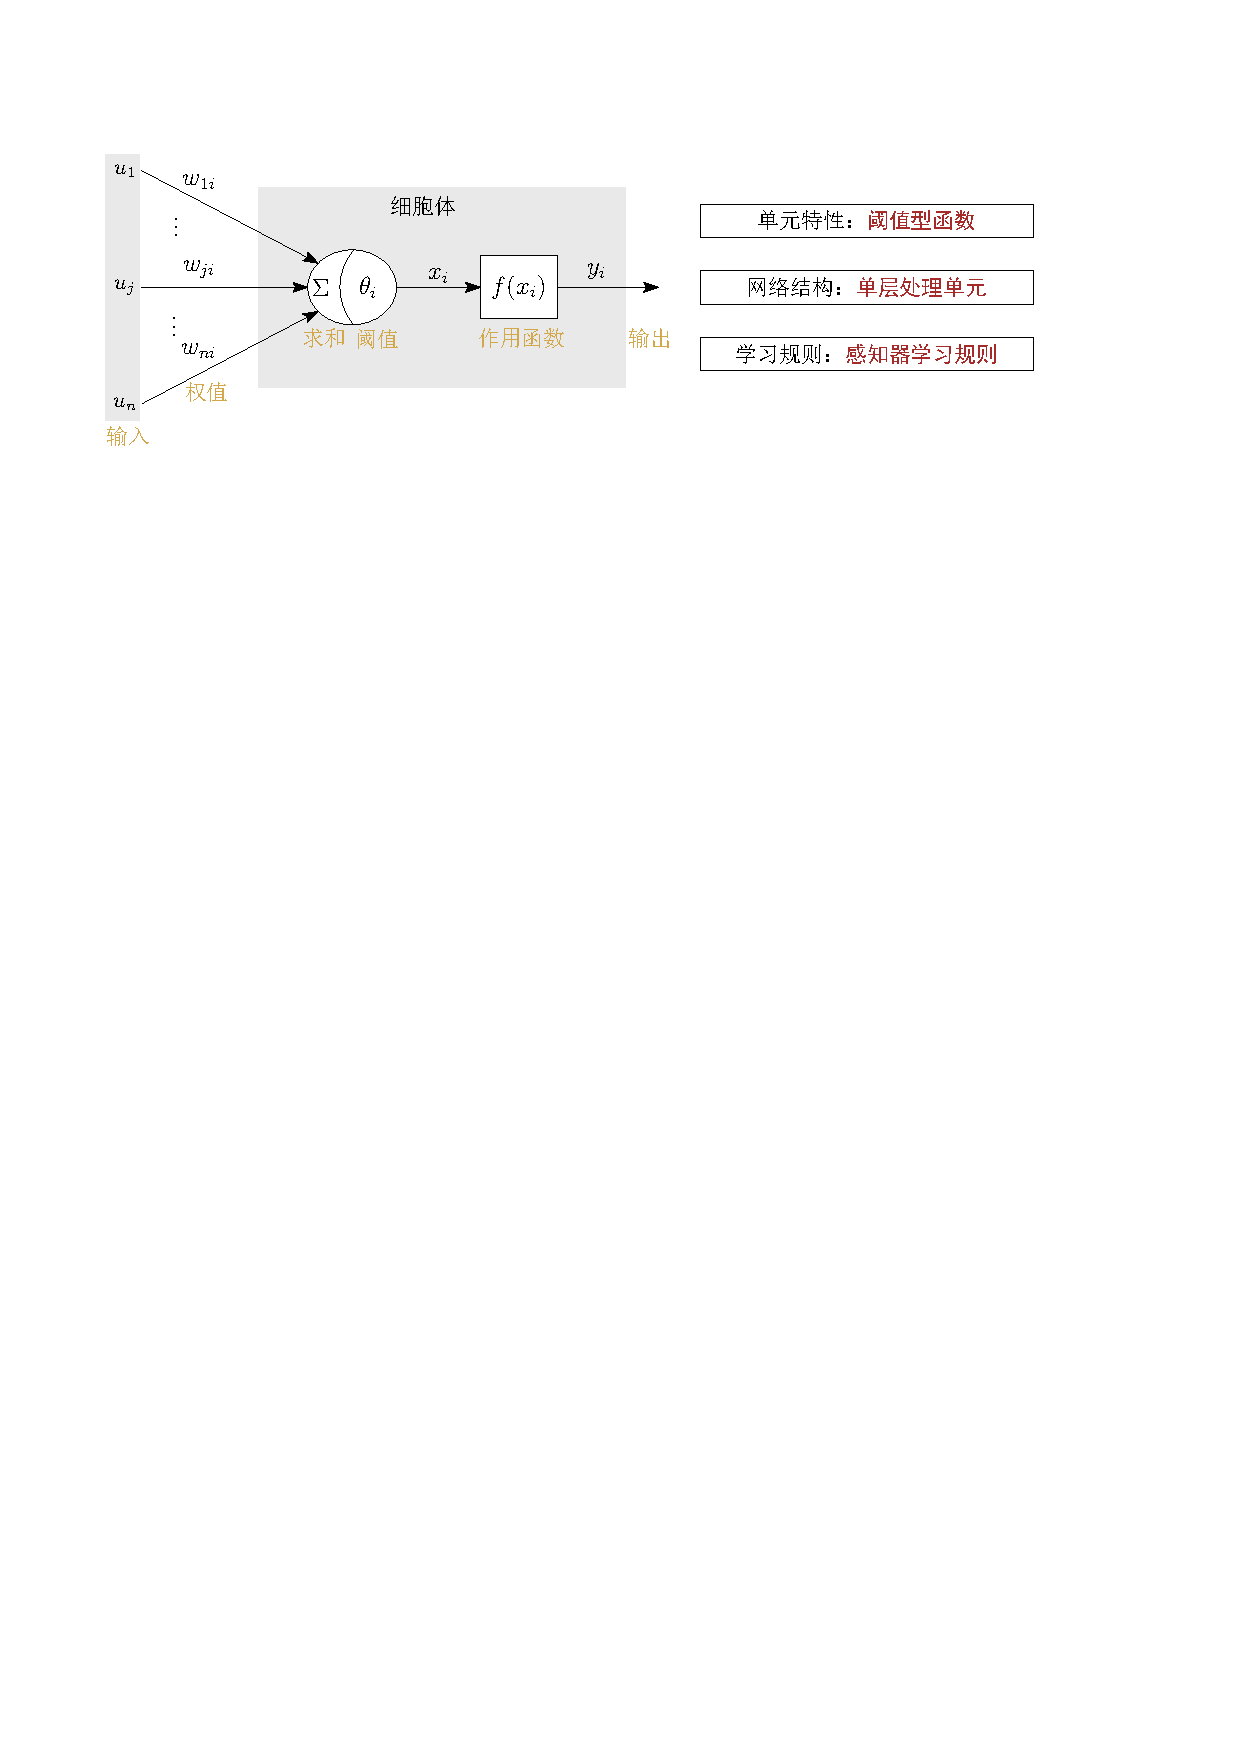
\includegraphics[width = .9\textwidth]{image/单层感知器的三要素.pdf}
\end{figure}
\begin{note}
    神经元单层特性:感知器是一种线性分类模型
    \begin{figure}[htbp]
        \centering
        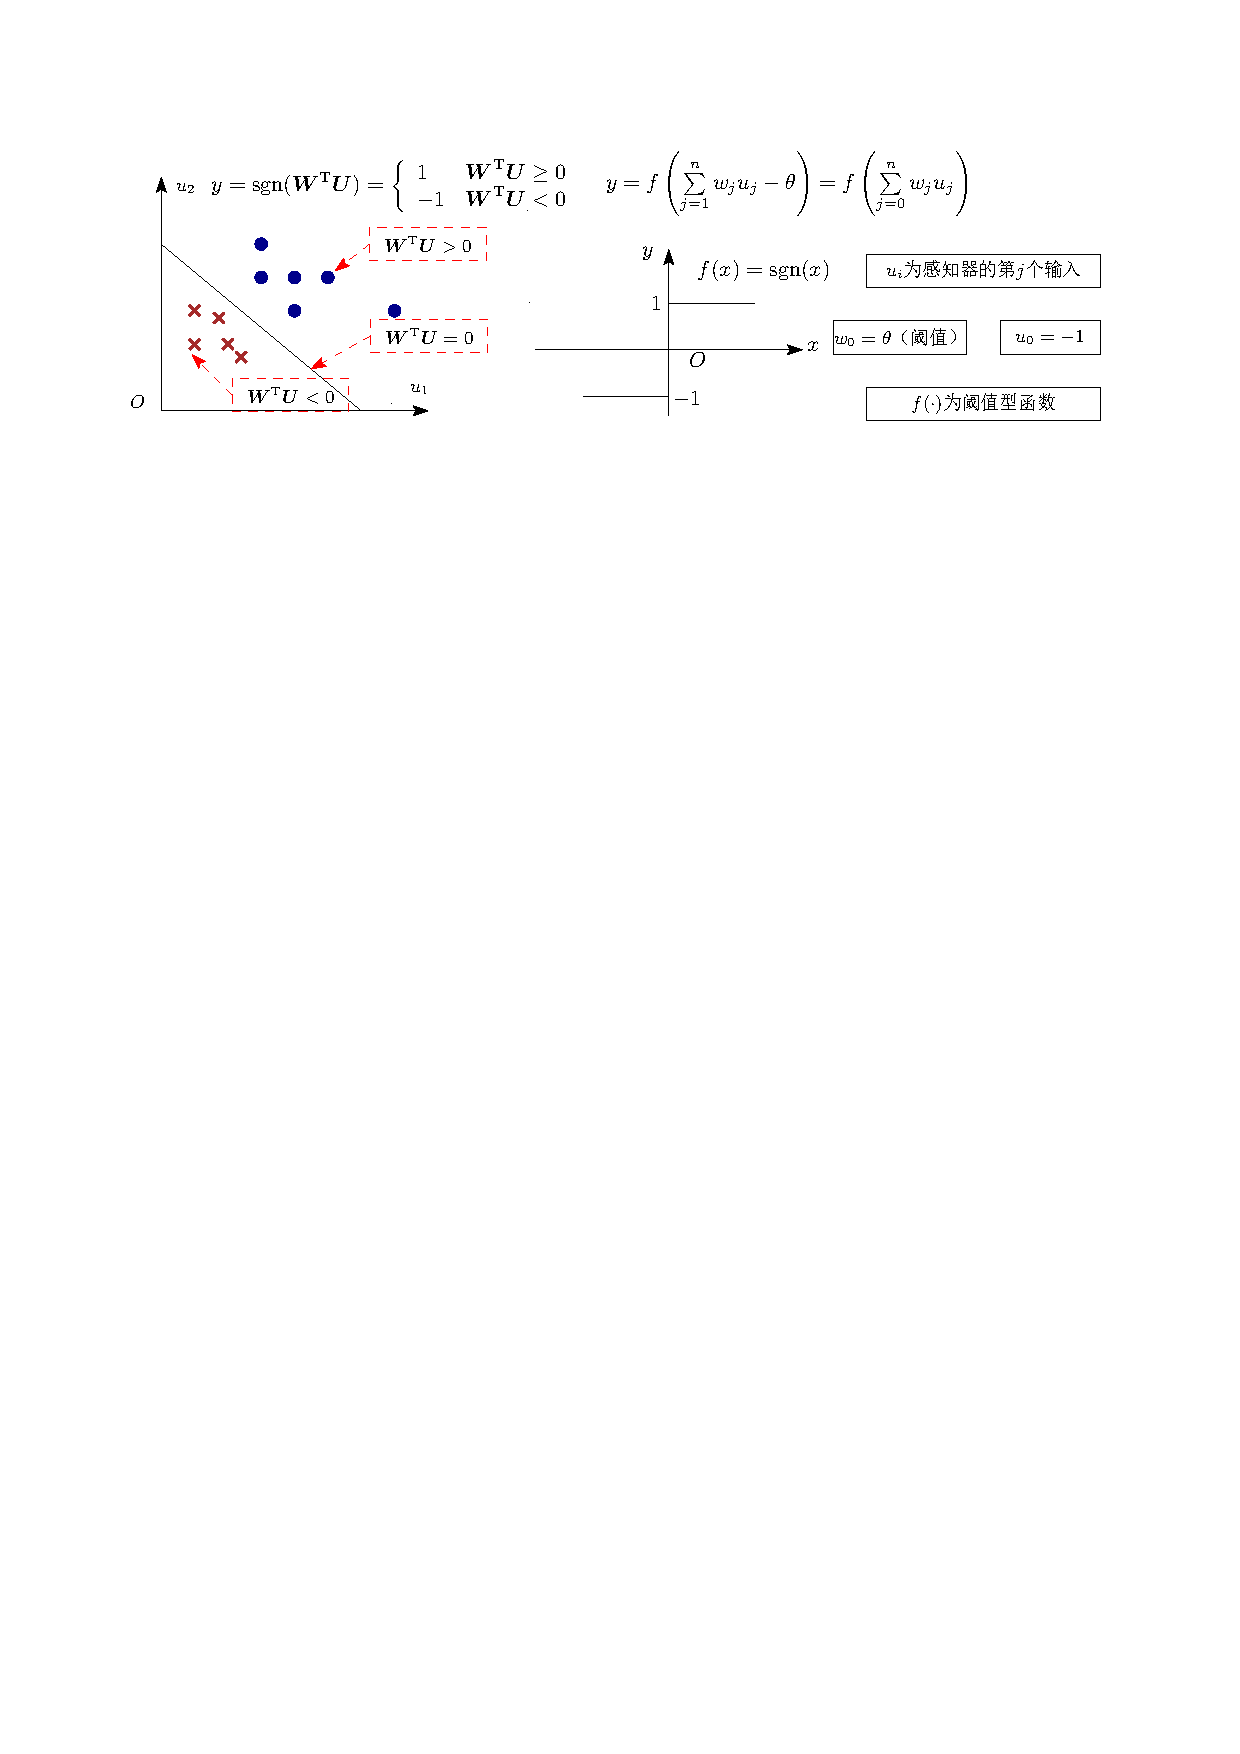
\includegraphics[width = .9\textwidth]{image/神经元单元特性.pdf}
    \end{figure}
\end{note}
\begin{example}
    若感知器输入为$n$维,输出为$m$维,那么可以实现将样本分为\underline{$2^m$}类
\end{example}
\begin{note}
    网络结构:单层处理单元
    \begin{figure}[htbp]
        \centering
        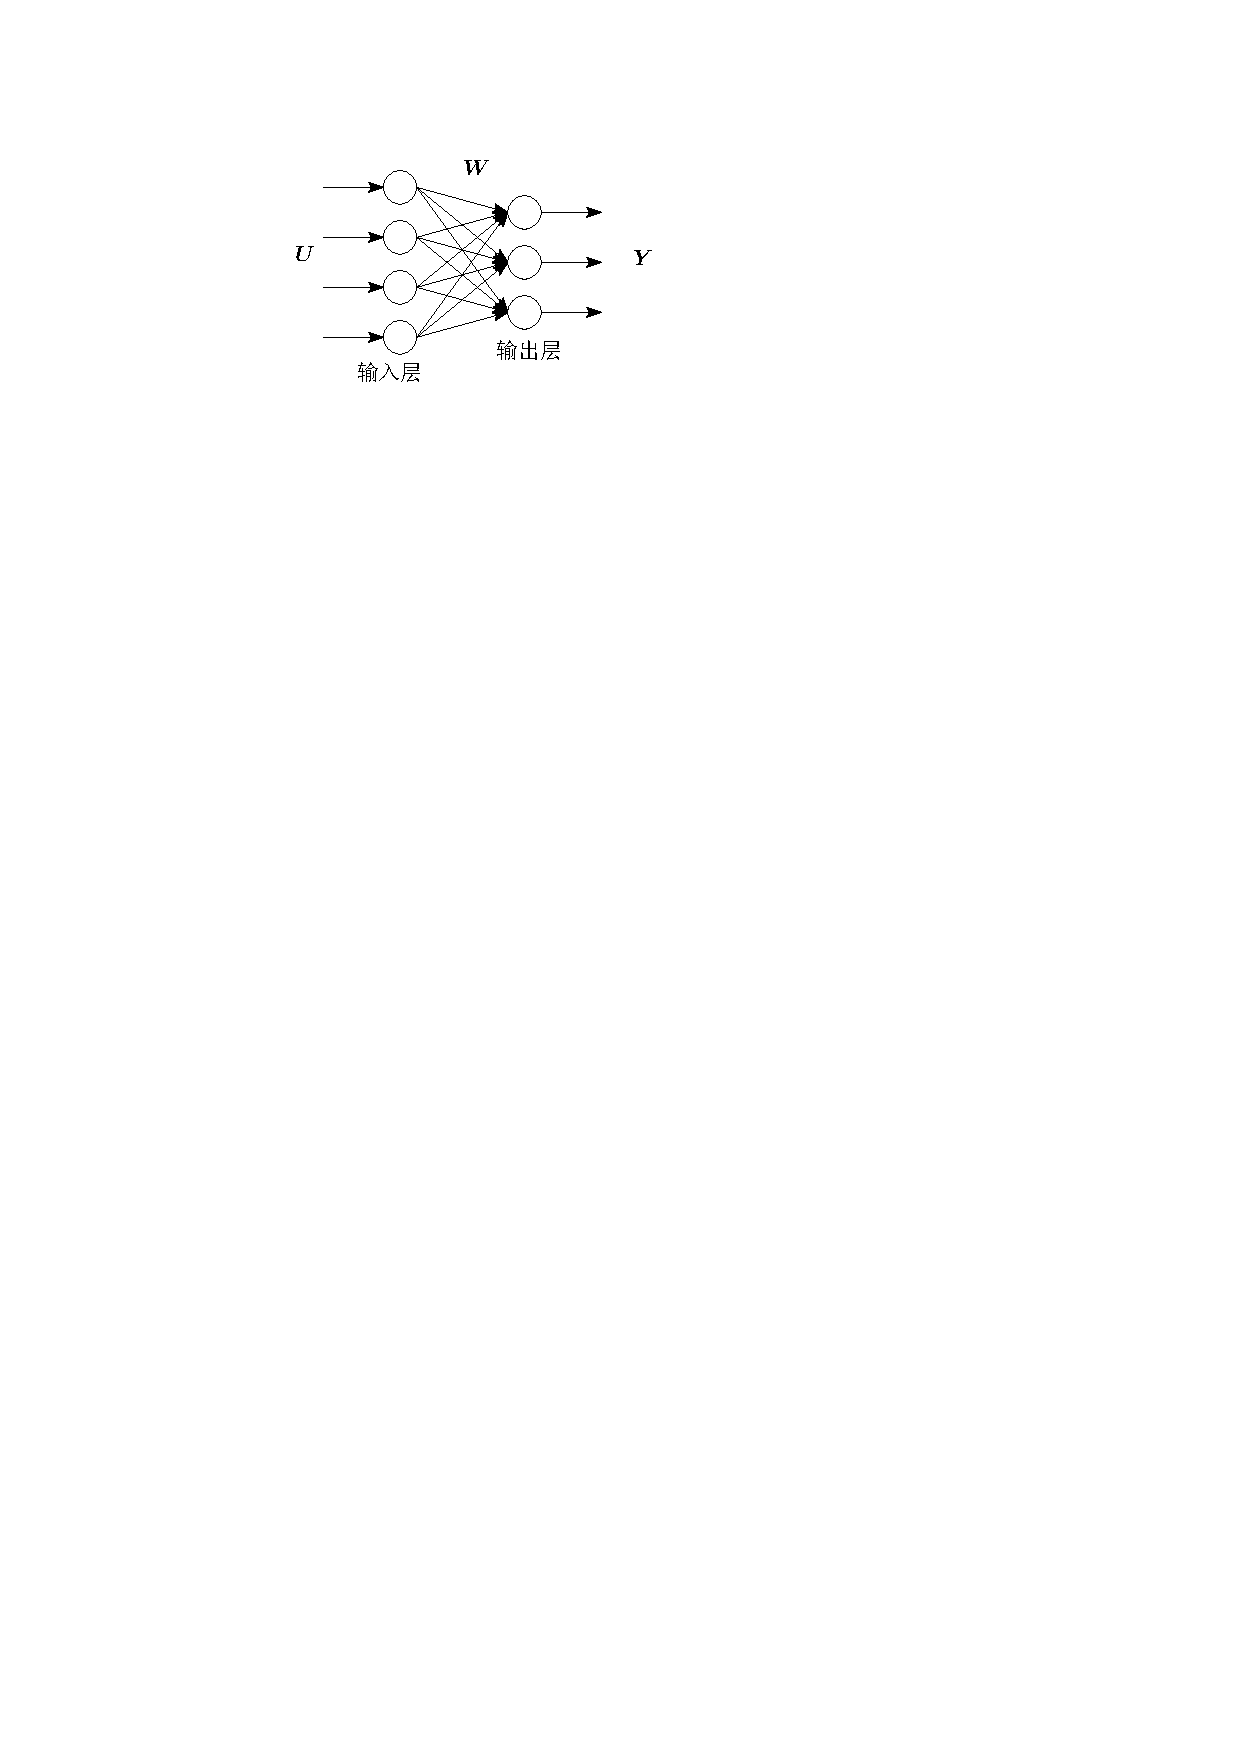
\includegraphics[scale = 0.9]{image/单层处理单元.pdf}
    \end{figure}
\end{note}

\begin{example}
    感知器学习规则是有监督的还是无监督的?
    \begin{enumerate}[A]
        \item \textcolor{main1}{有监督}
        \item 无监督
    \end{enumerate}
\end{example}

\begin{example}
    感知器学习得到的分类面是否唯一?
    \begin{enumerate}[A]
        \item 是
        \item \textcolor{main1}{否}
    \end{enumerate}
\end{example}
\begin{note}
    感知器学习规则:

    初始化权值向量$w_j (j = 0,1,\cdots,n)$,每分错一个样本,就用它来更新权值。权值调整规则为
    \[
        w_j(t+1) = w_j(t)+\eta\left( d_p-y_p(t) \right)u_{jp},\,\eta>0
    \]
    \begin{table}[htbp]
        \centering
        \begin{tabular}{|c|c|}
        \hline
        $\eta$ & 学习率 \\ \hline
        $d_p-y_p(t)$ & 学习误差:输出信号 \\ \hline
        $u_{jp}$ & 输入量 \\ \hline
        \end{tabular}%
    \end{table}%
\end{note}
感知器学习规则是$\delta$学习规则的一种特殊情况,它\textcolor{red}{不需要对作用函数求导数}。不仅学习速度较快,而且具有较高的精度。权值可以初始化为任意值。
\begin{example}
    单层感知器-或、异或
    \begin{enumerate}
        \item 单层感知器能否学习实现逻辑函数“或” 运算?为什么?
        \item 单层感知器能否学习实现逻辑函数“异或” 运算?为什么?
    \end{enumerate}
    \begin{figure}[htbp]
        \centering
        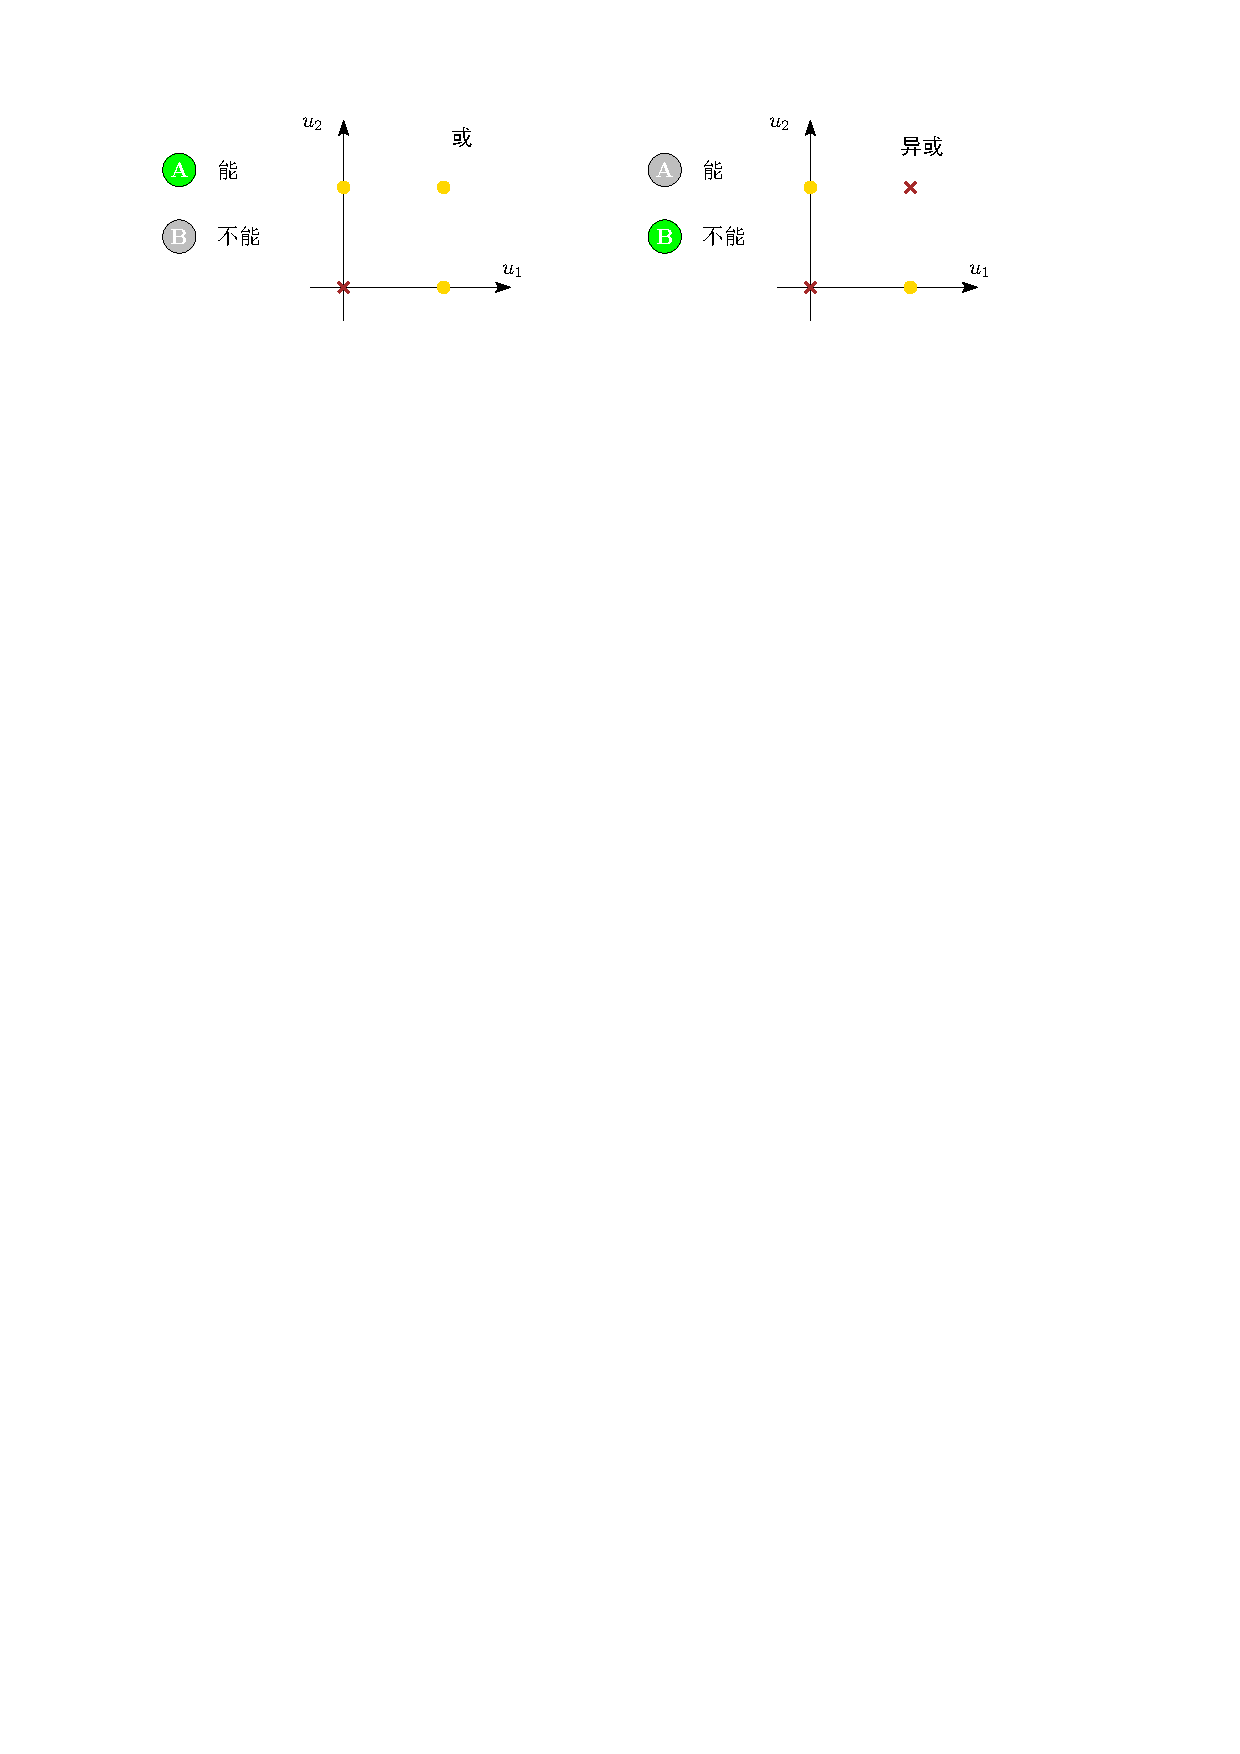
\includegraphics{image/单层感知器-或-异或.pdf}
    \end{figure}
\end{example}
\begin{note}
    单层感知器的局限性:
    \begin{itemize}
        \item 若输入的两类模式是线性可分集合(指存在一个超平面能将其分开),则算法一定收敛。
        \item 若输入模式为线性不可分集合,网络的学习算法不收敛,无法进行正确分类。
    \end{itemize}
\end{note}

\subsubsection{BP神经网络}
BP神经网络是一种特殊的多层感知器模型。
\begin{figure}[htbp]
    \centering
    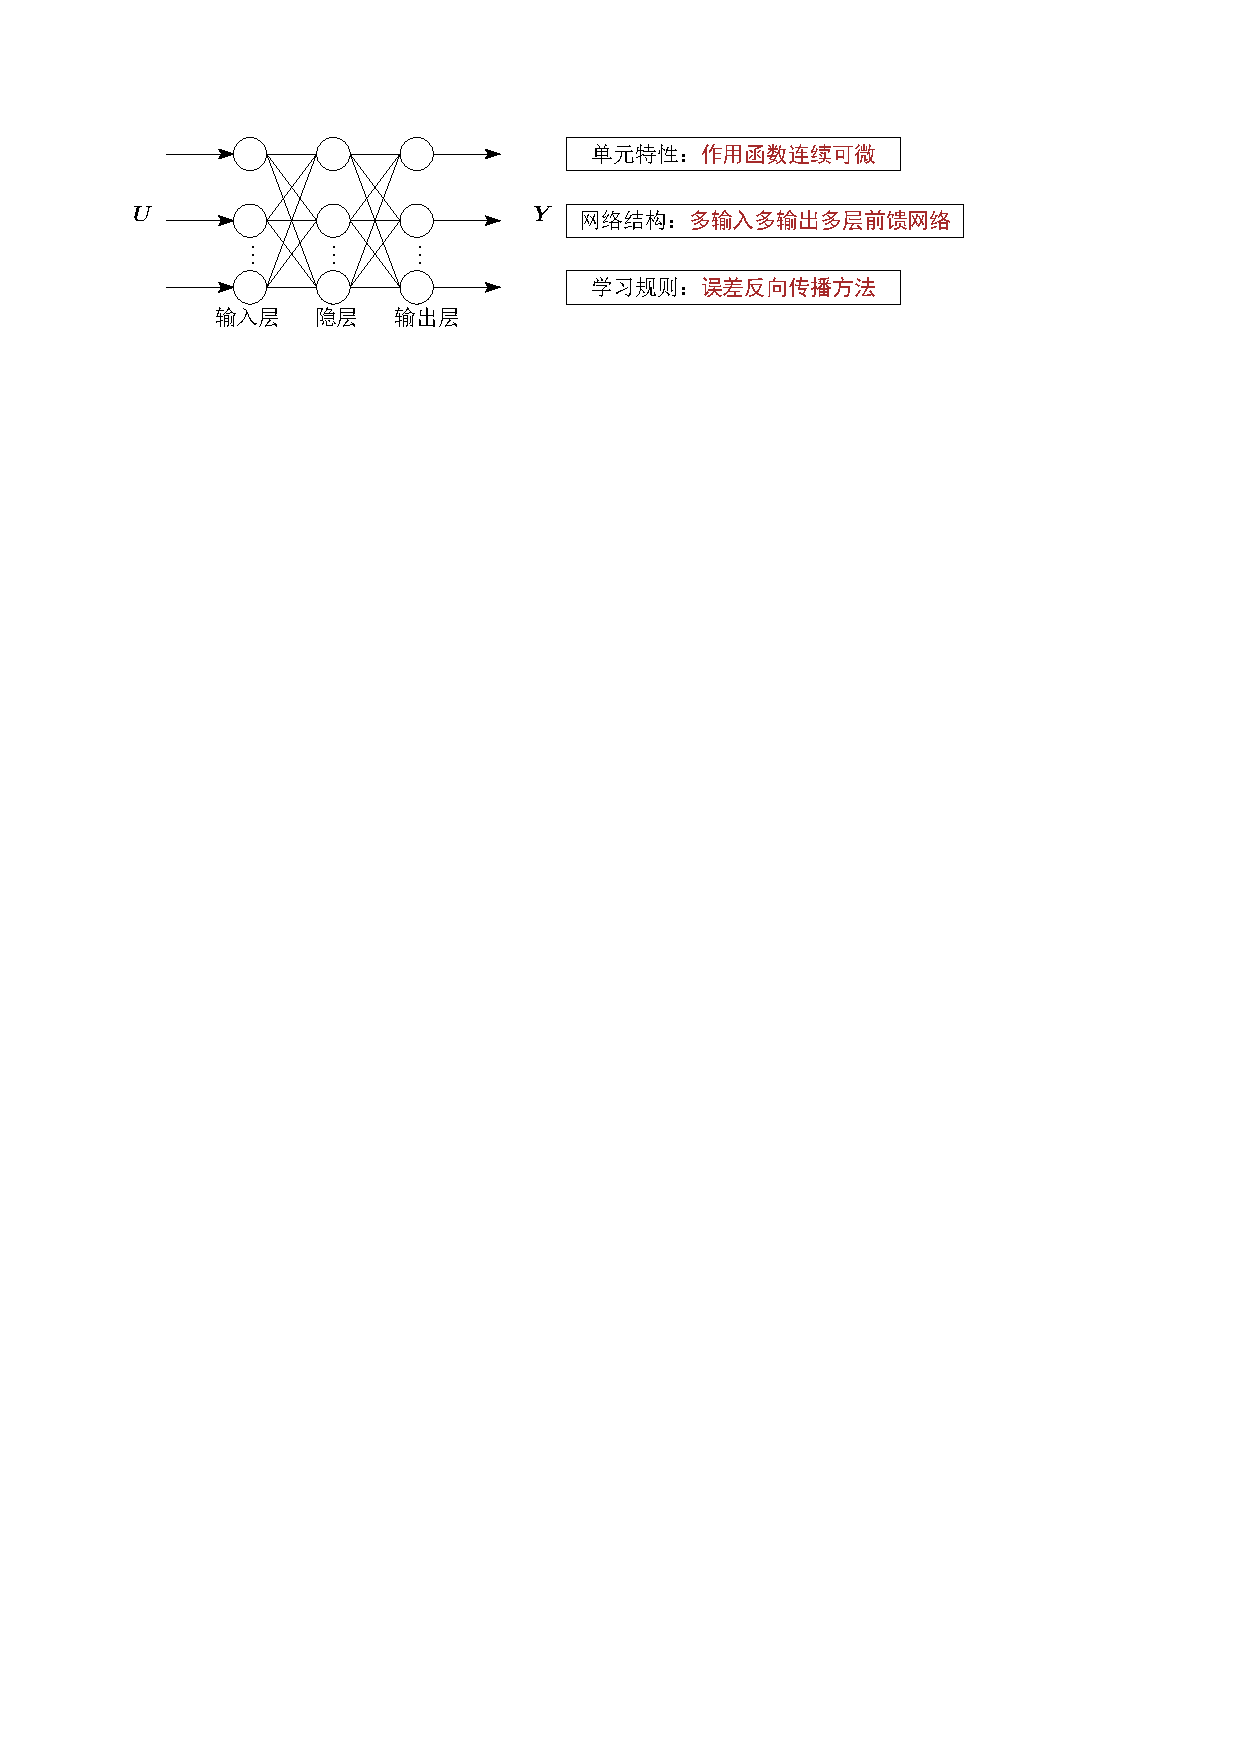
\includegraphics{image/BP神经网络的三要素.pdf}
\end{figure}
\begin{example}
    以下哪些神经元\textcolor{main1}{作用函数}是连续可微的?
    \begin{enumerate}[A]
        \item \textcolor{main1}{单极型Sigmoid 函数}
        \item \textcolor{main1}{双极型Sigmoid 函数}
        \item 阈值型函数
        \item 分段线性函数
    \end{enumerate}
    \begin{figure}[htbp]
        \centering
        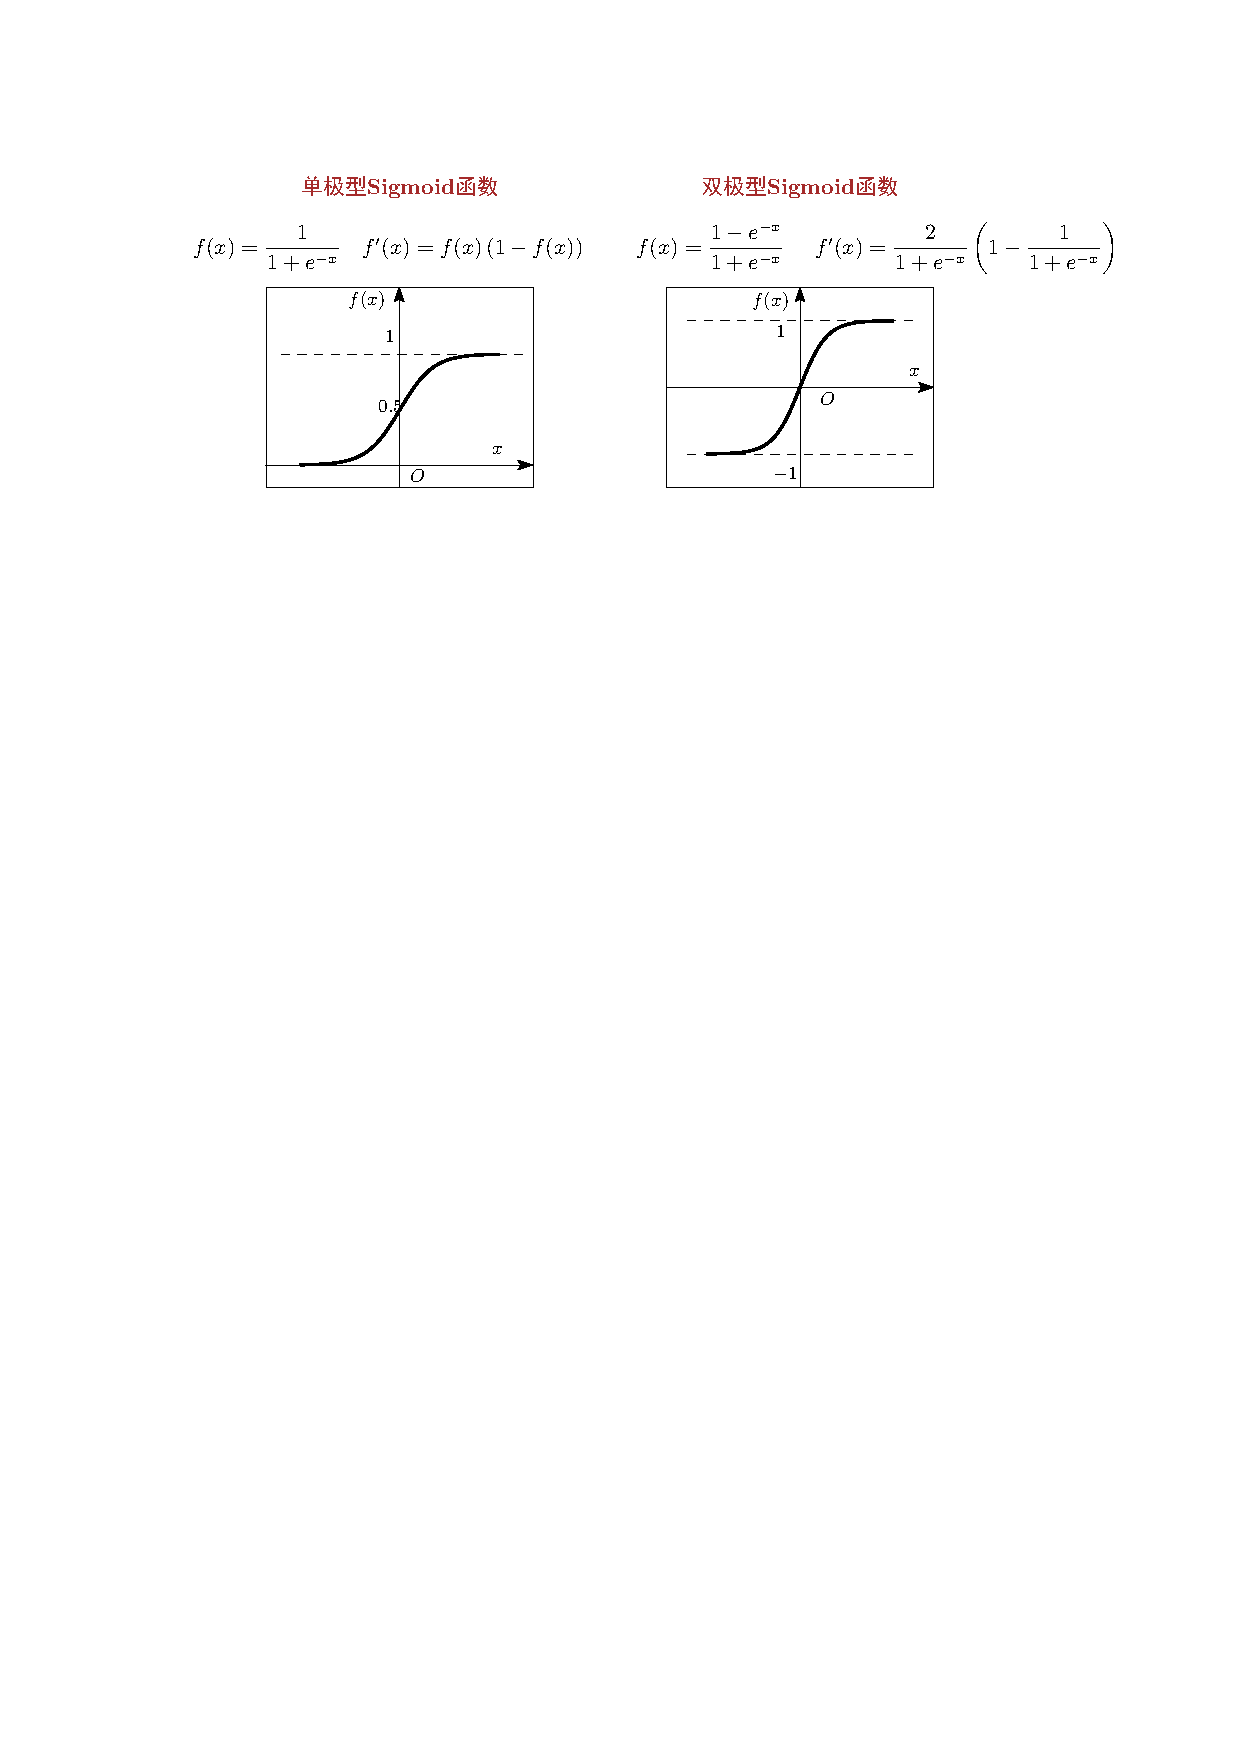
\includegraphics{image/BP-神经元作用函数.pdf}
    \end{figure}
\end{example}
\begin{note}
    BP 网络结构

    设网络的层数为$L$,第$l$层($0\leq l\leq L$)
    \begin{figure}[htbp]
        \centering
        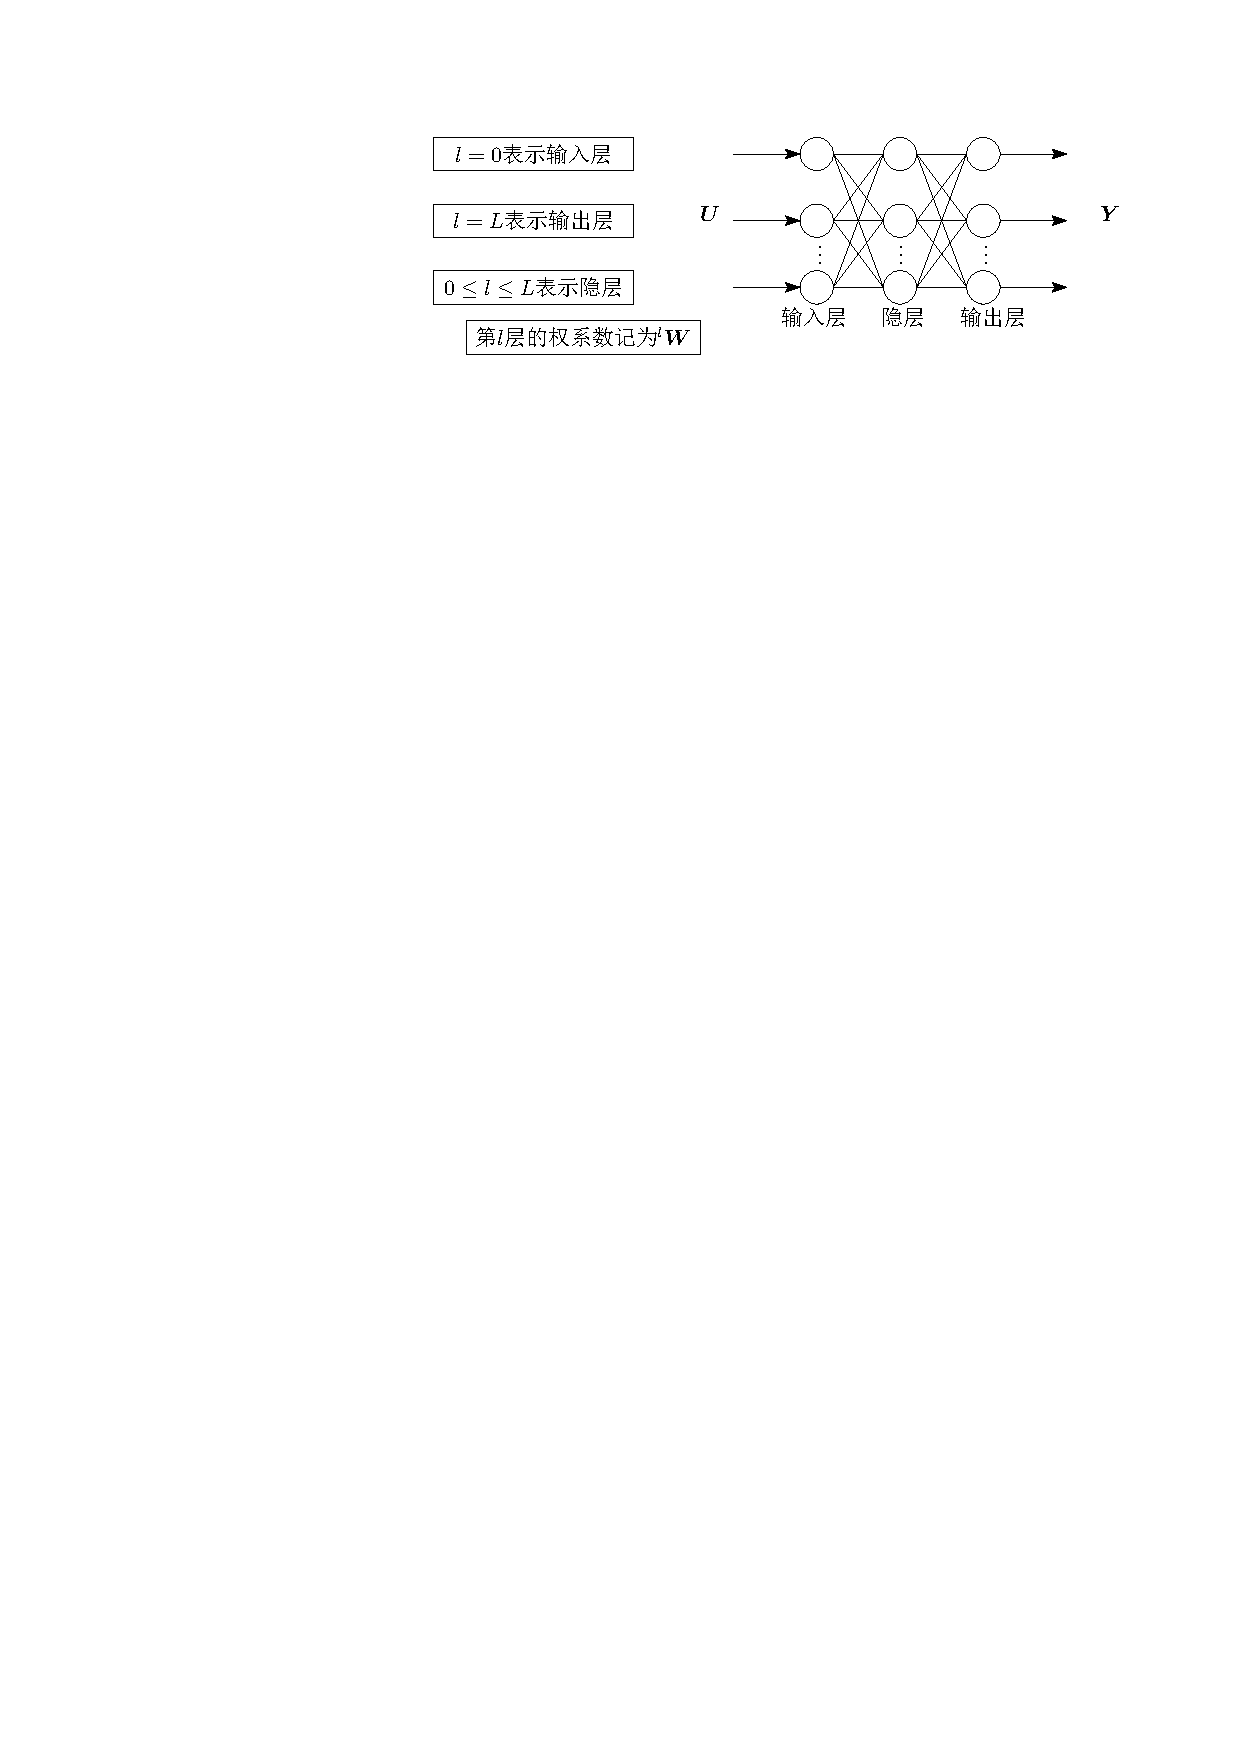
\includegraphics{image/BP网络结构.pdf}
    \end{figure}
\end{note}
\begin{note}
    BP 网络相关记号
    \begin{figure}[htbp]
        \centering
        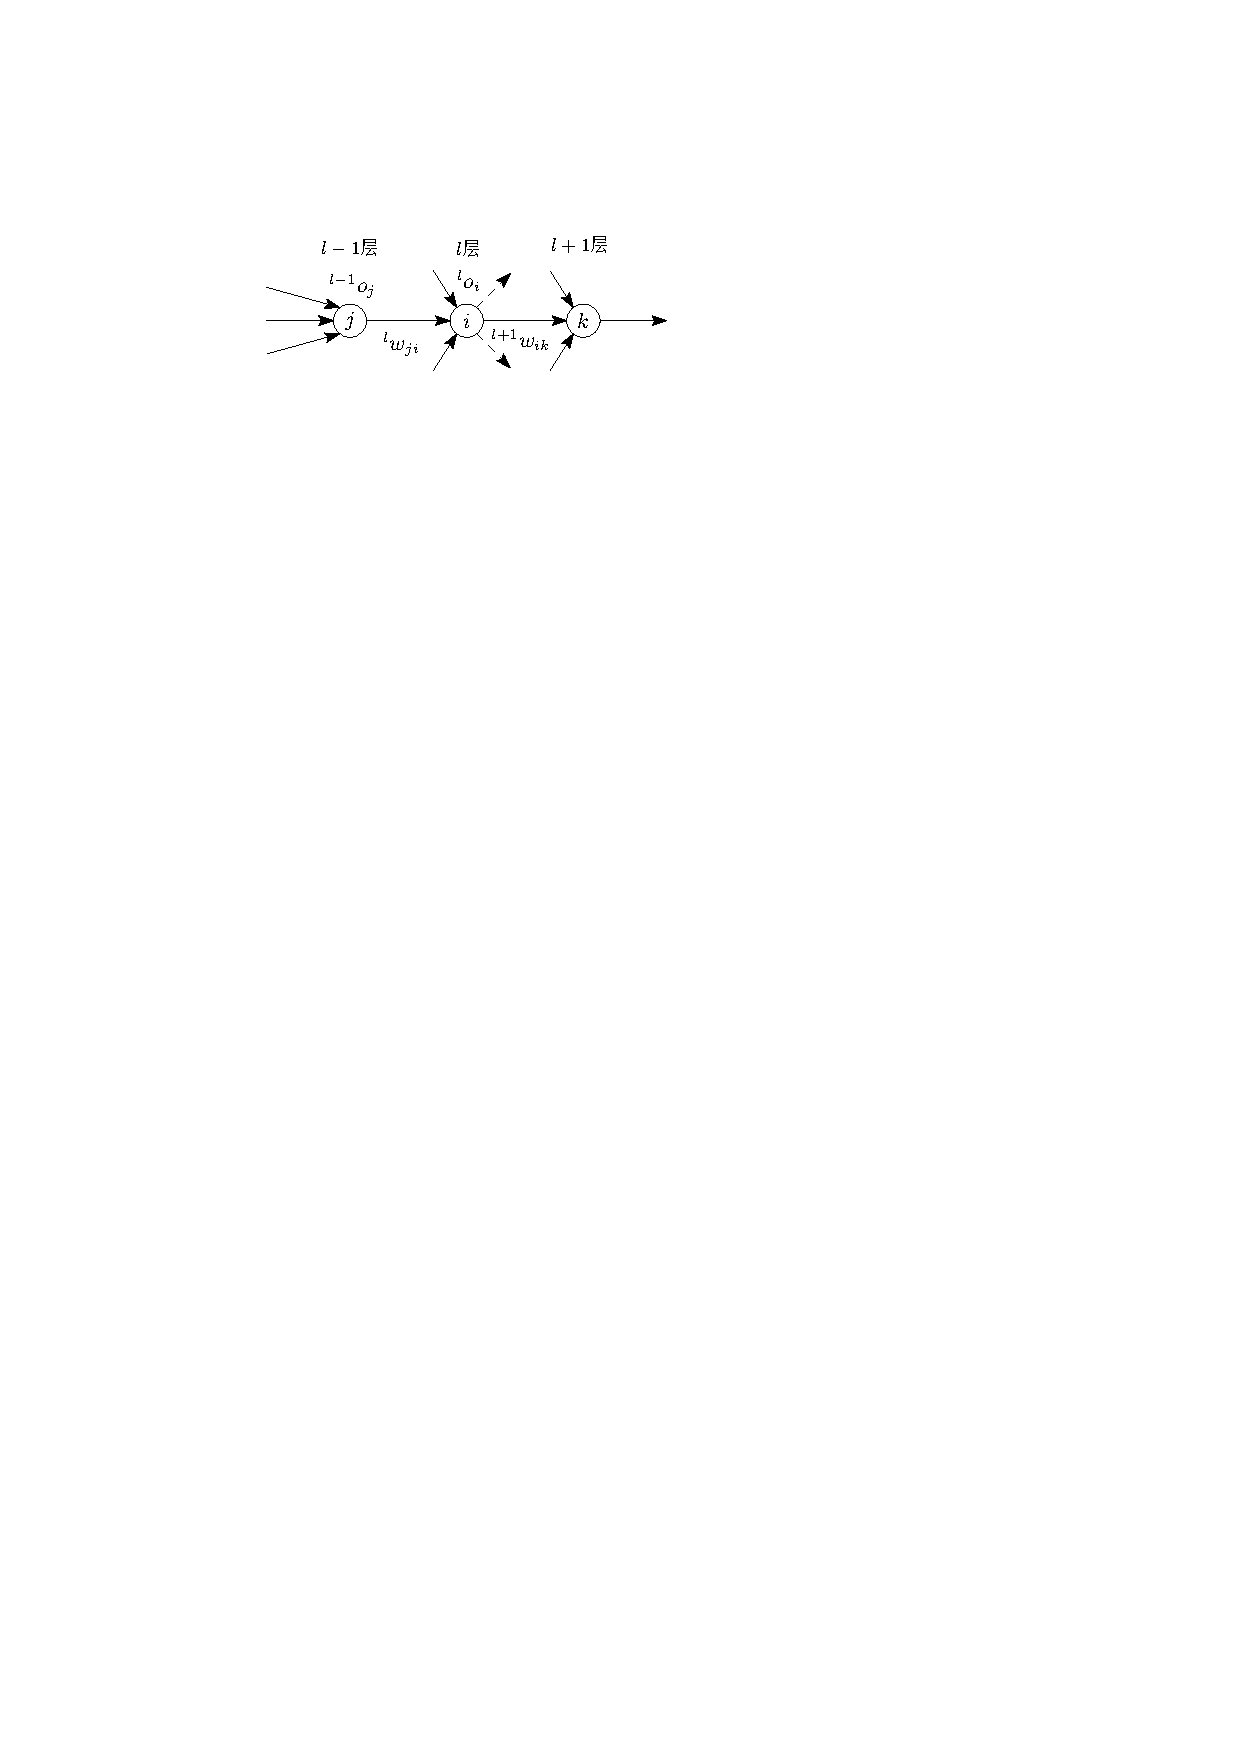
\includegraphics{image/BP网络相关记号.pdf}
    \end{figure}
    \begin{itemize}
        \item $^{l}o_{i} = f(^{l}x_i)$是神经元$i$的输出,$^{l}x_{i}$为净输入,$f(\cdot)$为作用函数
        \item $^{0}\boldsymbol{O} = \boldsymbol{u}$为输入信号,$^{L}\boldsymbol{O} = \boldsymbol{y}$为输出信号
        \item $^{l}w_{ji}$是$l-1$层第$j$个神经元与第$l$层第$i$个神经元的连结权值
        \item 对于BP网络,设输入向量$\boldsymbol{u}$是$n$维的,输出向量是$m$维的。已获得$P$个输入/输出样本对,记第$p$个样本为$\left\{ \boldsymbol{u}_p,\boldsymbol{d}_P \right\}$
    \end{itemize}
\end{note}
\begin{note}
    BP 学习的基本思想

    在外界输入样本的刺激下,不断改变网络的连接权值,使得网络的实际输出不断地接近期望的输出。
    \begin{figure}[htbp]
        \centering
        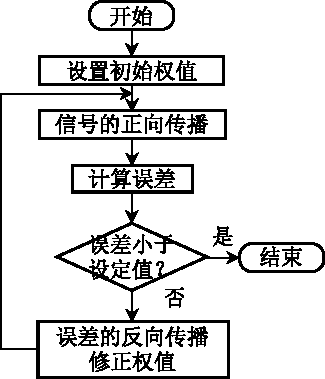
\includegraphics{image/BP学习的基本思想.pdf}
    \end{figure}
\end{note}
\begin{example}
    BP神经网络的学习方式是:
    \begin{enumerate}[A]
        \item \textcolor{main1}{有监督学习}
        \item 无监督学习
    \end{enumerate}
\end{example}
\begin{note}
    BP 学习的数学原理
    \begin{enumerate}
        \item 利用误差梯度修正权系数
        \[
            ^{l}w_{ji}(t+1) =\, ^{l}w_{ji}(t)-\eta\dfrac{\partial E_p}{\partial ^{l}w_{ji}},\,\eta>0
        \]
        \begin{figure}[htbp]
            \centering
            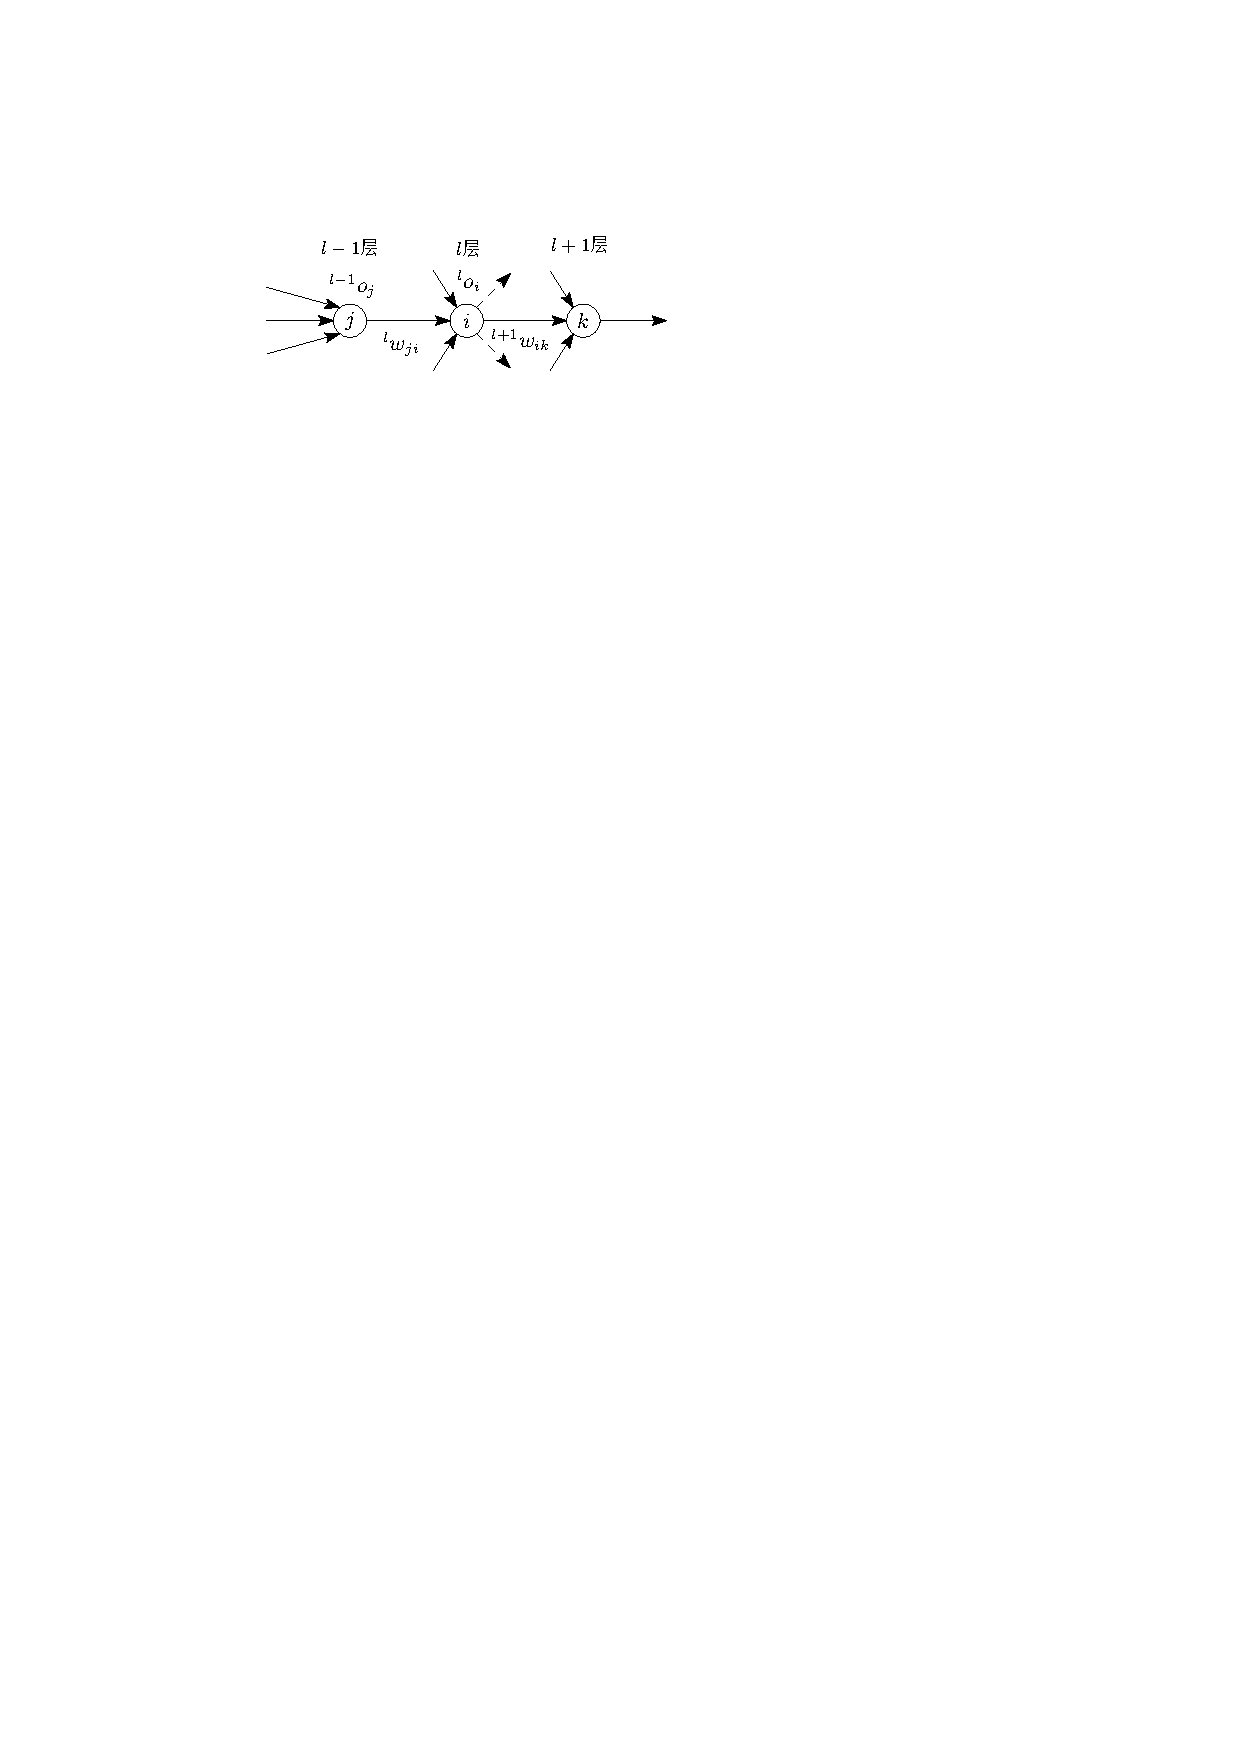
\includegraphics{image/BP网络相关记号.pdf}
        \end{figure}
        \[
            \dfrac{\partial E_p}{\partial ^{l}w_{ji}} = \dfrac{\partial E_p}{\partial ^{l}x_{ip}}\cdot \dfrac{\partial ^{l}x_{ip}}{\partial ^{l}w_{ji}} =\ ^{l}\delta\cdot\ ^{l-1}o_{jp}
        \]
        \item 输出误差
        \[
            E_{p} = \dfrac{1}{2}\sum\limits_{i = 1}^{m}\left( d_{ip}-y_{ip} \right)^2 =   \dfrac{1}{2}\sum\limits_{i = 1}^{m}\left( d_{ip}-f(\ ^{L})x_{ip} \right)^2  
        \]
        \item 输出层灵敏度
        \[
            ^{L}\delta_{ip} = \dfrac{\partial E_{p}}{\partial\ ^{L}x_{ip}} = -\left( d_{ip}-y_{ip} \right)\cdot f(\ ^{L}x_{ip})
        \]
        \item 对于非输出层(利用向量的链式法则)
        \[
            ^{l}\delta_{ip} = \dfrac{\partial E_{p}}{\partial\ ^{l}x_{ip}} = \left[ \dfrac{\partial\ ^{l+1}\boldsymbol{x}_p}{\partial\ ^{l}x_{ip}} \right]^{\mathrm{T}}\cdot \dfrac{\partial E_{p}}{^{l+1}\boldsymbol{x}_p}
        \]
        \begin{figure}[htbp]
            \centering
            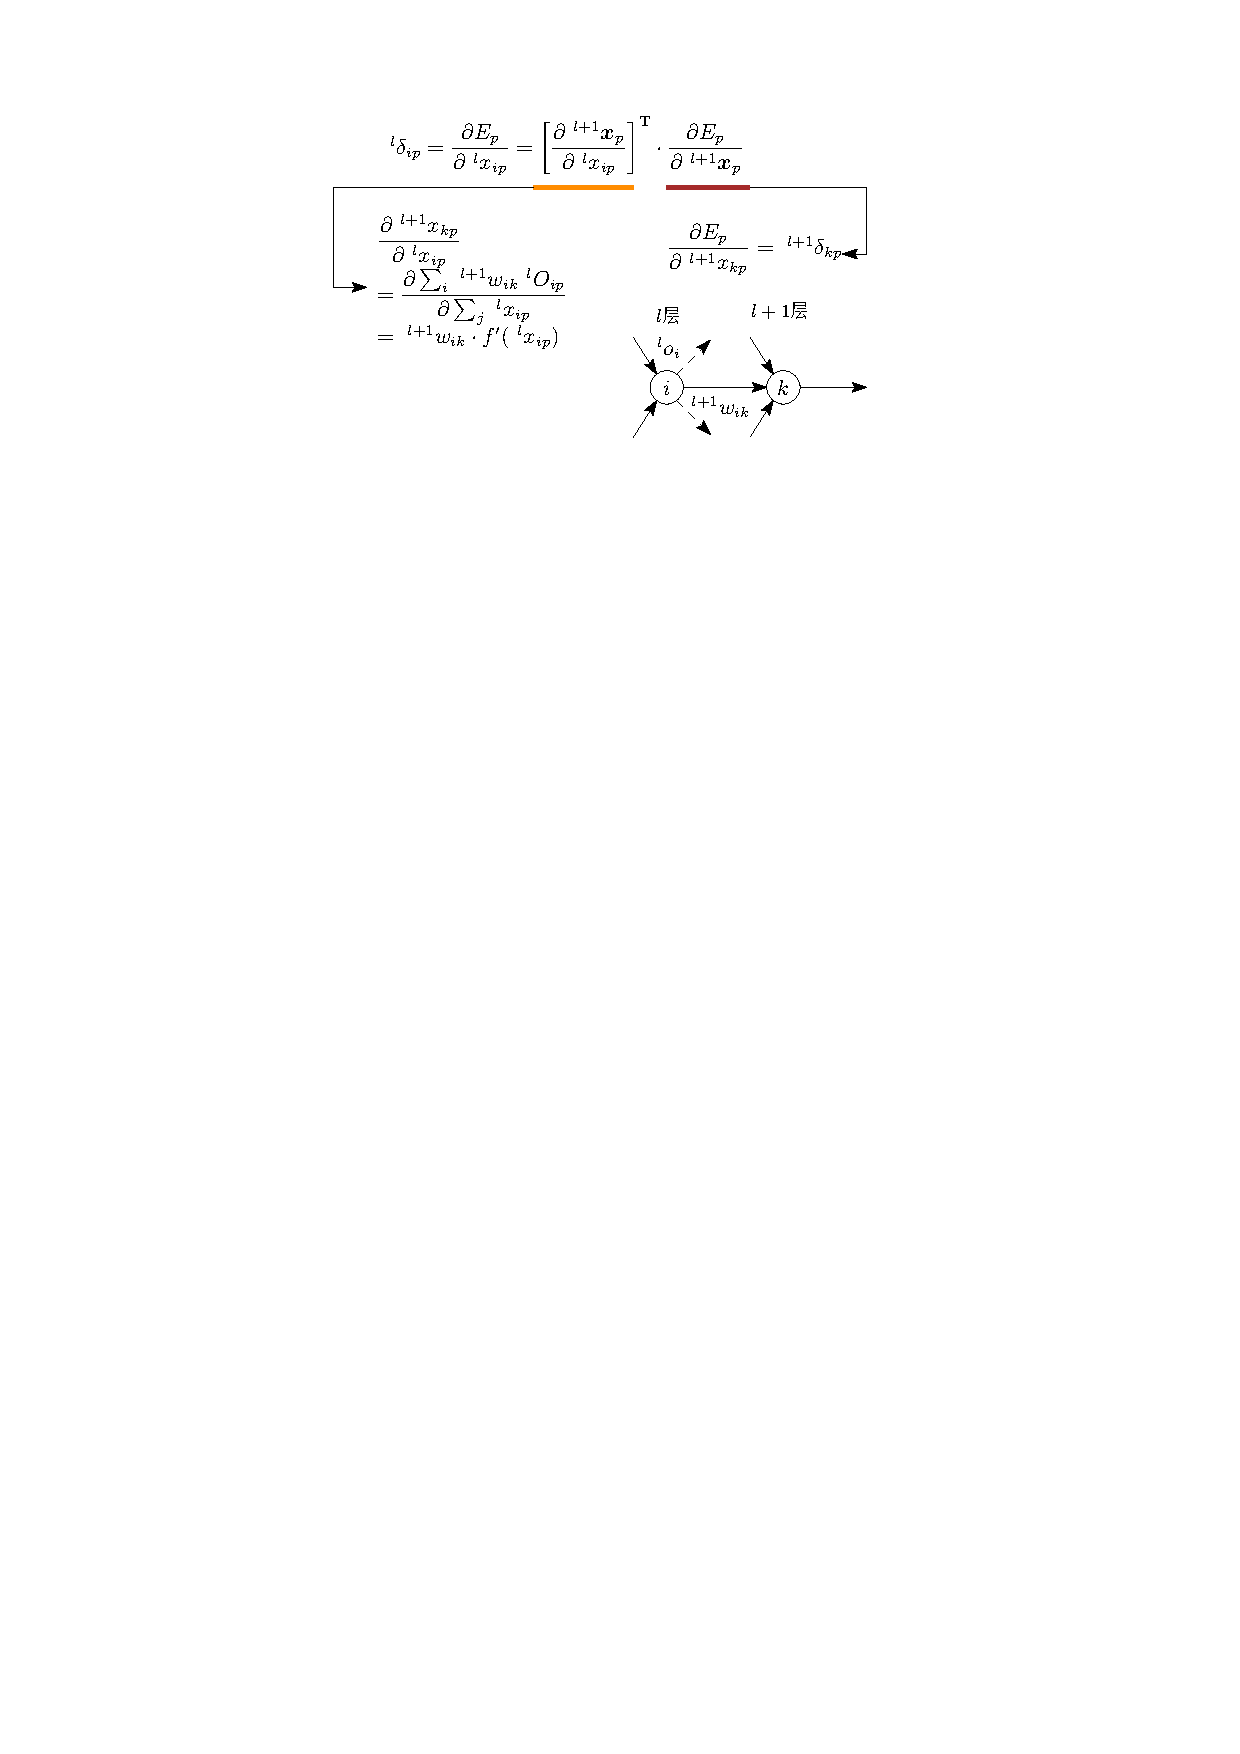
\includegraphics{image/BP的数学原理.pdf}
        \end{figure}
        \item $\delta$信号的BP过程
        \begin{figure}[htbp]
            \centering
            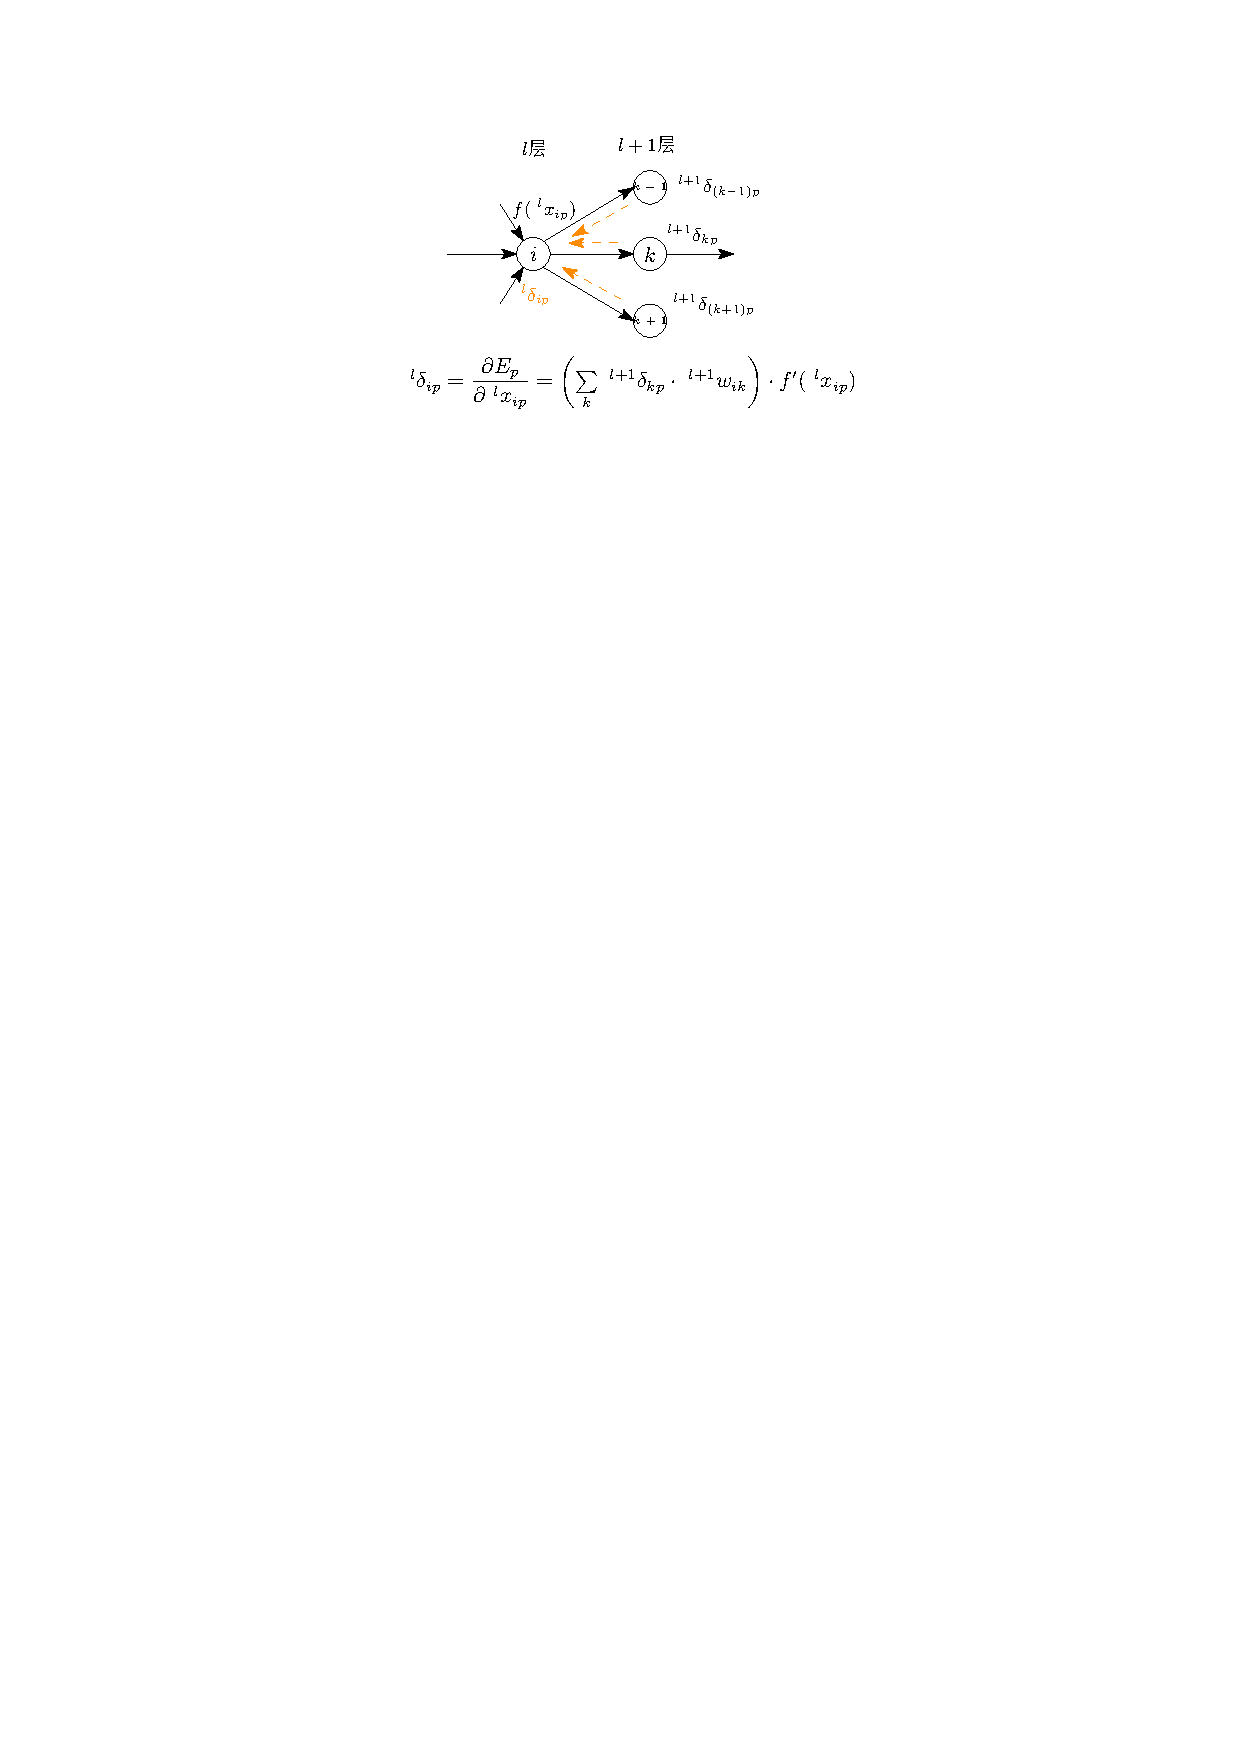
\includegraphics{image/delta信号的BP过程.pdf}
        \end{figure}
        \item $\delta$信号的反向传播
        \begin{itemize}
            \item 误差梯度
            \[
                \dfrac{\partial E_p}{\partial ^{l}w_{ji}} =\ ^{l}\delta\cdot\ ^{l-1}o_{jp}
            \]
            \item 输出层信号
            \[
                ^{L}\delta_{ip} = \dfrac{\partial E_{p}}{\partial\ ^{L}x_{ip}} = -\left( d_{ip}-y_{ip} \right)\cdot f(\ ^{L}x_{ip})
            \]
            \item 灵敏度
            \[
                ^{l}\delta_{ip} = \dfrac{\partial E_{p}}{\partial\ ^{l}x_{ip}}
            \]
            \item 其他层($\delta$信号反向传播)
            \[
                ^{l}\delta_{ip} = \dfrac{\partial E_p}{\partial\ ^{l}x_{ip}} = \left( \sum\limits_{k}\ ^{l+1}\delta_{kp}\cdot\ ^{l+1}w_{ik} \right)\cdot f'(\ ^{l}x_{ip})
            \]
            \item 权值调整公式
            \[
                \Delta \boldsymbol{W}(t) = \eta\left( d-y(t) \right)f'\left( x(t) \right)\boldsymbol{U}
            \]
        \end{itemize}
    \end{enumerate}
\end{note}
\begin{example}
    BP算法中的灵敏度$\delta $跟Delta($\delta$) 学习规则中的$\delta$ 的关联是:
    \begin{enumerate}[A]
        \item 两者没什么关系
        \item \textcolor{main1}{灵敏度$\delta$对应于$\delta$学习规则中的$\delta$}
    \end{enumerate}
\end{example}
\begin{example}
    基本BP算法步骤
    \begin{enumerate}
        \item 设置初始权值$\boldsymbol{W}(0)$为较小的随机非0值
        \item 给定输入/输出样本集合$\left\{ \boldsymbol{u}_{p},\,\boldsymbol{d}_{p} \right\}$,重复以下过程直至满足收敛条件$E_{\text{总}}\leq \varepsilon$
        \begin{itemize}
            \item 对于任意一个样本$p$,计算
            
            正向过程$\boldsymbol{u}_p,\,\cdots,\ ^{l-1}\boldsymbol{o}_{p},\,\ ^{l}\boldsymbol{x}_{p},\cdot,\boldsymbol{y}_{p} $

            反向过程
            \[
                \left\{
                    \begin{array}{l}
                        ^{L}\delta_{ip} = -\left( d_{ip}-y_{ip} \right)\cdot f'\left( \ ^{L}x_{ip} \right)\\
                        ^{l}\delta_{ip} = \left( \sum\limits_{k}\ ^{l+1}\delta_{kp}\cdot\ ^{l+1}w_{ik} \right)\cdot f'\left( \ ^{l}x_{ip} \right)\\
                        \dfrac{\partial E_{p}}{\partial\ ^{l}w_{ji}} = \ ^{l}\delta_{ip}\cdot\ ^{l-1}O_{jp}
                    \end{array}
                \right.
            \]
            \item 权值修正 $^{l}w_{ji}(t+1) = \ ^{l}w_{ji}(t)-\eta \dfrac{\partial E_{p}}{\partial\ ^{l}w_{ji}}$
        \end{itemize}
    \end{enumerate}
\end{example}
\begin{note}
    BP 网络的训练方式
    \begin{itemize}
        \item 串行方式
        
        每获得一个样本,就计算一次误差并更新权值
        \item 批量方式
        
        在所有样本输入后,根据总误差计算各层的误差信号并调整权值
    \end{itemize}
\end{note}
\begin{example}
    下列说法正确的是:
    \begin{enumerate}[A]
        \item \textcolor{main1}{串行方式需要的存储空间较少}
        \item 串行方式需要的计算量较少
        \item \textcolor{main1}{批量方式比串行方式更容易实现并行化}
        \item \textcolor{main1}{批量方式的学习速度往往优于串行方式}
    \end{enumerate}
\end{example}

